\documentclass[11pt]{article}
\usepackage[T1]{fontenc}
\usepackage{lmodern,microtype}
\usepackage[margin=1in,headheight=14pt]{geometry}
\usepackage{amsmath,amssymb,amsthm,mathtools}
\usepackage{booktabs,array,longtable,enumitem,graphicx}
\usepackage{xcolor}
\definecolor{navy}{RGB}{26,52,81}
\usepackage[hyphens]{url}% added 3 October 2026, batch 85B: long repository paths
\usepackage[colorlinks=true,linkcolor=navy,citecolor=navy,urlcolor=navy]{hyperref}
\usepackage{fancyhdr}
\pagestyle{fancy}\fancyhf{}
\fancyhead[L]{\small Matrix compositions: exact spectra and uniform asymptotics}
\fancyhead[R]{\small Research article}
\fancyfoot[C]{\thepage}
\setlength{\emergencystretch}{2em}
\setlist{itemsep=3pt,topsep=6pt}
\allowdisplaybreaks
\numberwithin{equation}{section}
\newtheorem{theorem}{Theorem}[section]
\newtheorem{proposition}[theorem]{Proposition}
\newtheorem{lemma}[theorem]{Lemma}
\newtheorem{corollary}[theorem]{Corollary}
\theoremstyle{definition}
\newtheorem{definition}[theorem]{Definition}
\newtheorem{question}{Research question}
\theoremstyle{remark}
\newtheorem{remark}[theorem]{Remark}
\newcommand{\E}{\mathbb E}
\newcommand{\Pp}{\mathbb P}
\newcommand{\N}{\mathbb N}
\newcommand{\dd}{\,\mathrm d}
\newcommand{\TV}{d_{\mathrm{TV}}}
\newcommand{\StirOne}[2]{\genfrac{[}{]}{0pt}{}{#1}{#2}}
\newcommand{\StirTwo}[2]{\genfrac{\{} {\}}{0pt}{}{#1}{#2}}
\DeclareMathOperator{\Pois}{Poisson}
\DeclareMathOperator{\Var}{Var}
\DeclareMathOperator{\Res}{Res}
\DeclareMathOperator{\Disc}{Disc}
\hypersetup{pdftitle={Matrix Compositions: Exact Spectra, Hankel Products, and Uniform Asymptotics},pdfauthor={Part I: OpenAI ChatGPT, research prepared for Vladimir Reshetnikov; Part II: research report prepared for Vladimir Reshetnikov},pdfsubject={OEIS A261781 and A261784; rigorous recurrence, determinant, coverage, and diagonal results; merged report a261781-matrix-compositions (batch 85B)}}
% Added 3 October 2026, batch 85B: finite tables of manuscript 01, shipped as data/01-two-poisson-*.tex
\makeatletter
\newcommand{\tableinput}[1]{\@@input #1 }
\makeatother

\title{\textbf{Matrix Compositions:\\ Exact Spectra, Hankel Products,\\ and Uniform Asymptotics}\\[8pt]
\large OEIS A261781, its empty-row transition,\\ and refined asymptotics for A261784\\[6pt]
\normalsize Part II: finite spectra, uniform asymptotics, and two Poisson limits}
\author{Part I: OpenAI ChatGPT\\\small Research prepared for Vladimir Reshetnikov\\[4pt]
\normalsize Part II: a research report prepared for Vladimir Reshetnikov}
\date{October 3, 2026 (Pacific time); merged 3 October 2026 (batch 85B)}
\begin{document}
\maketitle

\begin{abstract}
Let $T(n,k)$ count nonnegative integer matrices of total sum $n$, with $k$
ordered rows, an arbitrary number of ordered columns, and no zero row or
column. These are the entries of OEIS A261781. We establish a collection of
exact and asymptotic results for this family. First, its minimal eventual
constant-coefficient recurrence has order $k(k+1)/2$, and its full-rank
shifted Hankel determinants admit an explicit positive product formula,
including a polynomial refinement marking the number of columns. Second,
we give an exponential relative error bound for the unrestricted count that
is uniform in the number of rows. This yields a Poisson empty-row law at
$n=k(\log k+s)$, an explicit first correction with a summable error of
order $(\log k)^2/k^2$, and the sharp total-variation rate with its leading
constant. We also prove joint Gaussian--Poisson independence for column
count and empty-row count in this window. Third, for $n/k$ in compact
subsets of $(1,\infty)$, a positive Stirling-number transform gives a
uniform saddle expansion to every fixed order. For A261784, this identifies
the exact amplitude in the recorded leading equivalent and gives the first
relative correction. Finally, fixing the number of columns produces a
different explicit coverage threshold.

Attribution matters here: the generating functions, a recurrence of the
stated order, and fixed-row asymptotics were already published by Munarini,
Poneti, and Rinaldi. Thus the two conjecture labels still present in A261781
lead in part to a reconciliation with prior literature. The main extensions
of this article are the factored determinant and the uniform distributional
and asymptotic results. Full proofs, reproducible computations, a bounded
source audit, and further research questions are included. These are
unrefereed mathematical proofs; no proof-assistant verification or
historical-priority guarantee is claimed.
\end{abstract}

\paragraph{Editorial note (3 October 2026, batch 85B).}
This report is built from two manuscripts of ProveIt's incoming-reports
intake, written independently of each other on the same subject:
manuscript~06 of batch~85 (Part~I, the base, whose abstract stands above)
and manuscript~01 of batch~85 (Part~II). It is AI-assisted, unrefereed and
not formalized. Where the two manuscripts prove the same statement, it is
printed once, in Part~I, in manuscript~06's form, with a bracketed note
marked ``[Added 3 October 2026, batch 85B]'' that names manuscript~01's
version and its route; Part~II (Section~\ref{mxc:tp:sec:front} onwards)
prints everything that manuscript~01 adds. \emph{All of Part~II assumes
the column weight $u=1$}: manuscript~01 never weights columns.
The two manuscripts permute their Greek letters; everything here is
printed in manuscript~06's letters, and the dictionary of
Section~\ref{mxc:sec:dictionary} discloses every rename. Manuscript~01
presented its recurrence theorem as a proof of the OEIS order conjecture;
Munarini, Poneti and Rinaldi had already proved a recurrence of that order
with the same denominator \cite[Proposition~25 and Remark~26,
p.~16]{mpr2009}, so only its minimality is new
(Section~\ref{mxc:tp:sec:novelty}). Part~I's labels carry the prefix
\texttt{mxc:}, Part~II's the prefix \texttt{mxc:tp:}; Appendix~\ref{mxc:app:provenance}
records the provenance and every editorial change.

\newpage
\tableofcontents
\newpage

\part{Exact spectra, Hankel products, and uniform asymptotics}
\label{mxc:part:one}

\section{The problem, the sources, and the contribution}\label{mxc:sec:scope}

\subsection{Why this family is worth studying}
One generating function can behave quite differently when a parameter is
fixed or grows with the coefficient index. Matrix compositions provide an
especially explicit setting in which to study this difference. For fixed
$k$, the sequence is a finite sum of exponential terms and has an exact
linear recurrence. At $n\asymp k$, requiring every row to be used is a rare
event, and a saddle point governs its count. At $n=k(\log k+O(1))$, the
same requirement has a nondegenerate limiting probability. These regimes
cannot be interchanged by simply substituting a growing $k$ into a
fixed-$k$ asymptotic.

The current A261781 entry attributes to V\'aclav Kot\v{e}\v{s}ovec two
conjectures dated October 14, 2017: a column recurrence order
$k(k+1)/2$, and the limit $d(k+1)-d(k)\to1/\log 2$ for its exponential
growth constants \cite{oeis781}. Its companion A261780 counts the same
matrices while allowing zero rows \cite{oeis780}. The diagonal
$T(2N,N)$ is A261784 \cite{oeis784}.

\subsection{What was already known}
The primary enumerative source is \emph{Matrix Compositions} by Munarini,
Poneti, and Rinaldi \cite{mpr2009}, preceded by a 2006 conference paper
\cite{mpr2006}. In the 2009 article, Proposition~1 gives the generating
function, Propositions~12--13 give a root-of-unity formula and fixed-row
asymptotics, Propositions~22--24 give the no-zero-row inclusion--exclusion
formula, Proposition~25 gives a recurrence of order $\binom{k+1}{2}$,
and Proposition~29 gives the positive Stirling/Fubini transform used below.
Our elementary derivations of these identities make the article
self-contained; the identities themselves are attributed to those authors.

Louchard \cite{louchard} studies fixed-row probabilistic asymptotics,
including the number of columns and column-size statistics. An empty
\emph{column size} in that work is distinct from a zero \emph{row} here.
The A261784 entry already records a leading equivalent with numerical
amplitude and an explicit exponential constant, credited to
Kot\v{e}\v{s}ovec in 2017 and updated in 2024 \cite{oeis784}.

Accordingly, this article does not claim the discovery of the fixed-row
growth formula, recurrence existence, or the leading A261784 exponential
rate. The first OEIS statement receives an explicit minimality proof and a
careful indexing convention; the second follows from an already known
closed form. The stronger developments concern exact determinants and
uniform estimates as the number of rows grows.

\begin{table}[ht]
\centering\small
\begin{tabular}{@{}>{\raggedright\arraybackslash}p{0.28\textwidth}>{\raggedright\arraybackslash}p{0.33\textwidth}>{\raggedright\arraybackslash}p{0.32\textwidth}@{}}
\toprule
Topic & Existing foundation & Result established here\\
\midrule
Recurrences & Order-$\binom{k+1}{2}$ recurrence & Minimal eventual order; complete spectrum; initial impulse\\
Hankel determinants & Size-$k$ identity for unrestricted matrices & Factored size-$\binom{k+1}{2}$ determinant with column weights\\
Fixed-row asymptotics & Dominant pole and amplitude & Explicit error uniform in all $k\ge1$\\
Empty rows & Exact inclusion--exclusion & Poisson window, first correction, sharp total variation\\
Column count & Fixed-row Gaussian law & Joint Gaussian--Poisson limit; conditional limits\\
Diagonal A261784 & Recorded leading equivalent & Exact amplitude, first correction, uniform all-orders ray expansion\\
Fixed column count & Stars-and-bars enumeration & Explicit shifted coverage threshold when columns grow slowly\\
\bottomrule
\end{tabular}
\caption{Attribution and the scope of the extensions. ``Established here'' describes the proofs in this article, not a claim of priority over all literature.}
\label{mxc:tab:scope}
\end{table}

\subsection{Relation to ProveIt and the audit boundary}
The target was selected after inspecting the OEIS research in ProveIt
\cite{proveit}. Searches for A261780, A261781, and A261784 found no indexed
matching report. The relevant repository hit for matrix compositions was
a citation in the report on A260700 and parabolic double cosets, which
studies a different enumeration. The repository search exposed indexed
commit \texttt{ce37e13f4aa16819c87c3ccc611362d15758f2ac}; the search result
is not an exhaustive statement about every branch or historical archive.
No unformalized repository theorem is assumed in our proofs.

The source audit compared current OEIS records with the primary 2006,
2008, and 2009 works, and checked targeted searches for growing-row,
empty-row, and coupon-collection results. It found no matching statement
of the specific uniform expansions below. This is a bounded audit, so
the responsible claim is a set of fully specified results and proofs,
rather than a declaration of a historical breakthrough.

[Added 3 October 2026, batch 85B: the search statement describes the
pinned index \texttt{ce37e13f4}. At that commit manuscript~01, the source of
Part~II, had not yet arrived; it now forms Part~II of this report, which is
filed at
\path{SetTheory/Cardinals/docs/reports/generating-functions-and-asymptotics/oeis-sequence-asymptotics/a261781-matrix-compositions}.
Three repository neighbours bear on the method, and none is a dependency.
(i)~The report on A260700 \cite{pdc} uses the same two devices as
Section~\ref{mxc:sec:dense}, a uniform extraction of the Fubini pole at
$L$ (its Section~\texttt{pdc:sec:poles}) followed by an outer Stirling
transform (its Section~\texttt{pdc:sec:outer}), for a different sequence;
it cites \cite{mpr2009} as related work only. (ii)~The canonical
transseries volume proves the exact pole-lattice formula for the Fubini
numbers, its Theorem \texttt{q2:thm:fubini} \cite{tsvol}, of which the
estimate~\eqref{mxc:eq:fubini-estimate} is the one-pole truncation. (iii)~The
only ingredient of this report that is formalized anywhere in the
repository is the Fubini exponential generating function used in
Section~\ref{mxc:sec:dense}: the Lean declarations \texttt{Fabius.fubini}
(the definition $\mathsf F_q=\sum_bb!\StirTwo qb$),
\texttt{Fabius.egfA\_fubini} and
\texttt{Fabius.two\_sub\_exp\_mul\_egfA\_fubini}, the identity
$(2-e^t)\sum_q\mathsf F_qt^q/q!=1$, in
\path{Analysis/FabiusFunction/Lean/FabiusFunction/OrderedBell.lean}
\cite{leanob}. Nothing else stated in either Part is formalized, and
placement beside the repository's formal projects confers no formal
status.]

\subsection{Notation and conventions}
Throughout, $n$ is total matrix mass, $k$ is the number of rows, and $C$ is
the number of columns. Unless stated otherwise, $M$ denotes the number of
zero rows in an unrestricted uniformly chosen matrix. Write
\[
 L=\log 2,\qquad
 a_k=2^{-1/k},\quad r_k=1-a_k,\quad
 d_k=r_k^{-1},\quad c_k=\frac{a_k}{2kr_k}.
\]
The empty-row window uses $h=n/k$ and $\eta=k e^{-h}$. The dense-ray
regime uses $\lambda=n/k$ and a saddle $r>0$; these are separate local
notations. The falling factorial is $(x)_j=x(x-1)\cdots(x-j+1)$.
All logarithms are natural. Constants in uniform big-$O$ notation may
depend on the fixed compact sets specified in each theorem.

We include one empty matrix at $n=0$ for each fixed height when zero rows
are allowed. Thus $A(0,k)=1$, $A(n,0)=0$ for $n>0$,
$T(0,0)=1$, and $T(0,k)=0$ for $k>0$. These conventions matter for
recurrences and Hankel rank at the initial index.

\subsection{Notation dictionary for the two manuscripts}\label{mxc:sec:dictionary}
[Added 3 October 2026, batch 85B.] Manuscripts~06 (Part~I) and~01
(Part~II) use the same objects but different letters, and three Greek
letters are cyclically permuted between them: manuscript~06's $\eta$,
$\lambda$, $\rho$ are manuscript~01's $\lambda$, $\rho$, $\eta$. Copying a
formula from one manuscript into the other without translation therefore
gives a formula that is wrong, not merely differently named. This report
prints \emph{everything} in manuscript~06's letters. Table~\ref{mxc:tab:dictionary}
lists every symbol of manuscript~01 that was renamed for Part~II and Part~I's
notes, with the tempting false reading where one exists; manuscript~01's
other symbols are unchanged. Normalizations are unchanged throughout:
every rename is a change of letter only. All of Part~II is at column
weight $u=1$, so its $A$, $T$, $c_k$, $d_k$ are the unweighted ones of
Part~I.

{\small
\setlength{\LTcapwidth}{\textwidth}
\begin{longtable}{@{}>{\raggedright\arraybackslash}p{0.30\textwidth}>{\raggedright\arraybackslash}p{0.16\textwidth}>{\raggedright\arraybackslash}p{0.12\textwidth}>{\raggedright\arraybackslash}p{0.33\textwidth}@{}}
\caption{Manuscript~01's symbols and the letters used for them in this
report. ``False reading'' gives what the manuscript-01 letter means in
this report.}\label{mxc:tab:dictionary}\\
\toprule
Notion & This report (ms.~06) & Ms.~01 & False reading if copied\\
\midrule
\endfirsthead
\toprule
Notion & This report (ms.~06) & Ms.~01 & False reading if copied\\
\midrule
\endhead
\bottomrule
\endfoot
Matrices allowing zero rows & $A(n,k)$ & $U(n,k)$ & ---\\
Its generating function & $F_k(z;1)$ & $U_k(z)$ & ---\\
Zero rows of an unrestricted matrix & $M$ & $Z_{n,k}$ & ---\\
Poisson mean $ke^{-n/k}$ & $\eta$ & $\lambda$ & $\lambda$ is $n/k$ on dense rays\\
Ratio $n/k$ on compact rays & $\lambda$ & $\rho$ & $\rho$ is the pole-bound ratio\\
Pole-bound ratio $L/\sqrt{L^2+8}$ & $\rho$ & $\eta$ & $\eta$ is the Poisson mean\\
Dense-ray saddle, $r/(1-e^{-r})=\lambda$ & $r$ & $\tau$ & $\tau$ is a formal variable in \eqref{mxc:eq:saddle-algorithm}; ms.~01's $r$ is $n-k$ or a moment index\\
Half-saddle mass $Lr/2$ & $v$ & $\mu$ & $\mu_k(u)$ is an amplitude in Theorem~\ref{mxc:thm:uniform} and a column mean in \eqref{mxc:eq:column-constants}\\
Fixed-$k$ constants & $c_k$, $d_k$; $d(x)$ at real $x$ & $c(k)$, $d(k)$, $d(x)$ & ---\\
Diagonal index & $N$, $a_N=T(2N,N)$ & $m$, $a(m)$ & $m$ indexes $d_m$ and counts columns in Section~\ref{mxc:sec:fixedcolumns}\\
Diagonal constants & $c_*$, $d_*$ & $c$, $d$ & $c_k$, $d_k$ are the fixed-$k$ constants\\
Diagonal corrections & $\beta_1=\beta$, $\beta_2$, $\beta_3$ & $\delta_1$, $\delta_2$, $\delta_3$ & ms.~01's ``$\beta_1$'' is $\widetilde\beta_1=\beta_1+\tfrac16$, a different constant\\
Saddle correction coefficients & $E_j(\lambda)$ & $A_m(\rho)$ & $A(n,k)$ is a count\\
Leading saddle approximation & $\mathcal B(n,k)$ & $B(n,k)$ & $B$, $B(u)$ are pole-bound constants\\
Truncation order of an expansion & $J$ & $M$ & $M$ is the zero-row count\\
Coverage correction polynomials & $\mathcal Q_j(h,\eta;L)$ & $Q_j(h,\lambda;L)$ & $Q_q(d)$, $Q_{k,u}(z)$, $Q$ are other objects\\
Coverage exponent & $\Psi(j,h,\epsilon)$, $\epsilon=1/k$ & $G(r,h,\varepsilon)$ & ---\\
Moment index; point mass & $j$; $m$ & $r$; $t$ & $r$ is the saddle\\
Reduced denominator; its degree & $Q_{k,1}(z)$; $D$ & $D_k(z)$; $N_k$ & $D$ is also $n-Q$ in Section~\ref{mxc:sec:dense-columns}\\
Denominator coefficients & $q_i$ & $d_r$ & $d_k$ is a growth constant\\
Roots and roots of unity & $a_j=2^{-1/j}$, $z_{j,\ell}$, $\omega_j$ & $q_j$, $r_{j,h}$, $\zeta_j$ & $q_i$ are denominator coefficients\\
Fubini numbers & $\mathsf F_q$ & $F_j$ & $F_k(z;u)$ is a generating function\\
Entire Stirling kernel; its coefficients & $\mathsf W_n(w)$; $\chi_{n,\ell}$ & $W_n(v)$; $w_{n,\ell}$ & $W_N$ is a diagonal diagnostic, $w_{j,\lambda}$ a Hankel weight\\
Kernel variable; Euler operator & $w=Lz$; $D_w$ & $v$; $D_v$ & $v=Lr/2$\\
Kernel correction polynomials & $P_r(w)$ & $p_r(v)$ & $P_j(t)$ in Section~\ref{mxc:sec:hankel} is another polynomial\\
Kernel-proof variable $1/n$ & $\epsilon$ & $h$ & $h=n/k$\\
Kernel-proof auxiliaries & $\Sigma_j(n)$, $\mathsf a_j$, $\mathsf e_\ell$, $\mathsf r_\ell$, $\mathsf b_r$, $\Pi_r(\ell)$, $\mathbf B_a$, $\delta_0$ & $S_j(n)$, $A_j$, $E_\ell$, $R_\ell$, $B_r$, $P_r(\ell)$, $B_a$, $\delta$ & $E_j(\lambda)$, $R_p(w)$, $B$, $\delta$ of Lemma~\ref{mxc:lem:kernel}\\
Gaussian functional & $\mathcal G_b$ & $\mathfrak G_b$ & ---\\
Cumulant recursion & $\mathcal K_j(z,a)$ & $K_j(z,a)$ & $K$ is a compact set of rays\\
Stirling index; Stirling defect & $Q_{n,k}$; $\Delta_{n,k}=n-Q_{n,k}$ & $J_{n,k}$; $\Delta_{n,k}$ & $J_q$ is a block count; $\Delta_{n,k}$ is Section~\ref{mxc:sec:dense-columns}'s $D$\\
Defect generating variable & $\xi$ & $u$ & $u$ is the column weight\\
Smooth comparator; its root & $\mathcal A^{[J]}(x)$; $x_J(Y)$ & $A^{[M]}(x)$; $x_M(Y)$ & ---\\
Inverse core & $\Lambda$, $\varpi=W_0(\alpha\Lambda)$ & $X$, $w$ & $X$ is a Poisson or normalized variable, $w$ a PGF or kernel variable\\
Integer threshold; its bracket & $\mathcal N(Y)$; $\epsilon_J$, $C_J$ & $N(Y)$; $\varepsilon_M$, $C_M$ & $N$ is the diagonal index\\
$\log 2$ & $L$ & $L$, macro \texttt{\textbackslash Li} & ---\\
\end{longtable}
}

\section{Exact enumeration and the complete spectrum}\label{mxc:sec:exact}

\begin{definition}
A matrix composition of mass $n$ and height $k$ is a $k\times C$ matrix
of nonnegative integers with positive column sums and total entry sum $n$.
Its columns and rows are ordered. Let $A(n,k)$ count these matrices, and
let $T(n,k)$ count those with every row nonzero.
\end{definition}

The word interpretation in A261781 is equivalent: a column of sum $i$
specifies the multiplicities of the $k$ letters in an alphabetically
ordered word of length $i$. Every letter occurs somewhere precisely when
every row is nonzero. For example, $T(2,2)=3$: the one-column matrix
with entries $1,1$, and the two $2\times2$ permutation matrices.

\subsection{Generating functions and a positive transform}
Let $u>0$ mark columns. Define
\[
 A(n,k;u)=\sum_B u^{C(B)},\qquad
 T(n,k;u)=\sum_{B:\,M(B)=0}u^{C(B)}.
\]
At $u=1$ these reduce to the unweighted counts. A nonzero column has
generating function $(1-z)^{-k}-1$, since a column of sum $i$ has
$\binom{i+k-1}{i}$ possibilities. Taking an ordered sequence of columns
gives the classical identity
\begin{equation}\label{mxc:eq:gf}
 F_k(z;u):=\sum_{n\ge0}A(n,k;u)z^n
 =\frac{1}{1-u((1-z)^{-k}-1)}
 =\frac{(1-z)^k}{(1+u)(1-z)^k-u}.
\end{equation}
This also gives the positive recurrence
\begin{equation}\label{mxc:eq:positive-rec}
 A(n,k;u)=u\sum_{i=1}^n\binom{i+k-1}{i}A(n-i,k;u)
 \qquad(n\ge1,k\ge1).
\end{equation}
Deleting any designated set of zero rows proves inclusion--exclusion:
\begin{equation}\label{mxc:eq:ie}
 T(n,k;u)=\sum_{j=0}^k(-1)^{k-j}\binom{k}{j}A(n,j;u).
\end{equation}
Equations~\eqref{mxc:eq:gf}--\eqref{mxc:eq:ie} are established enumeration,
not new formulas \cite{mpr2009,oeis780,oeis781}.

For later use let $\mathsf F_q=\sum_{b=0}^q b!\StirTwo{q}{b}$ be the
ordered Bell or Fubini number, with $\mathsf F_0=1$. The two Stirling
triangles satisfy
\[
 x(x+1)\cdots(x+n-1)=\sum_q\StirOne{n}{q}x^q,
 \qquad
 (e^z-1)^k=k!\sum_{q\ge k}\StirTwo{q}{k}\frac{z^q}{q!}.
\]
Expanding \eqref{mxc:eq:gf} at $u=1$ in powers of $(1-z)^{-k}$ gives
\[
 A(n,k)=\frac12\sum_{b\ge0}2^{-b}\binom{n+kb-1}{n}
 =\frac1{n!}\sum_{q=0}^n\StirOne{n}{q}\mathsf F_q k^q.
\]
For $n>0$ the $b=0$ term is zero. The identity
$\mathsf F_q=\frac12\sum_{b\ge0}b^q2^{-b}$ follows by comparing the
exponential generating functions, with the usual $0^0=1$ convention.
Applying the $k$th binomial difference to $j^q$ yields
\begin{equation}\label{mxc:eq:stirling}
 \boxed{\displaystyle
 T(n,k)=\frac{k!}{n!}\sum_{q=k}^n
    \StirOne{n}{q}\StirTwo{q}{k}\mathsf F_q.}
\end{equation}
This is Proposition~29 of \cite{mpr2009}. Its nonnegative summands
will allow controlled asymptotic replacement without alternating-sum
cancellation. In particular $T(n,n)=\mathsf F_n$.

\subsection{Every pole survives}
For fixed $u>0$ put
\[
 b=\frac{u}{1+u},\qquad L_u=\log(1+1/u),\qquad
 a_{j,u}=b^{1/j},\qquad \omega_j=e^{2\pi i/j}.
\]
The denominator in $F_j(z;u)$ has simple zeros
$z_{j,\ell}=1-a_{j,u}\omega_j^\ell$, $0\le\ell<j$.
Their residues are $-a_{j,u}\omega_j^\ell/((1+u)j)$.
Consequently, for $n\ge1$,
\begin{equation}\label{mxc:eq:weighted-binet}
 A(n,j;u)=\frac{a_{j,u}}{(1+u)j}
  \sum_{\ell=0}^{j-1}\omega_j^\ell
     (1-a_{j,u}\omega_j^\ell)^{-n-1}.
\end{equation}
The polynomial part of $F_j$ is the constant $1/(1+u)$, so
\eqref{mxc:eq:weighted-binet} is deliberately stated only for $n\ge1$.
Its unweighted specialization is the published Binet formula
\cite[Proposition~12]{mpr2009}.

\begin{theorem}[Minimal recurrence and spectrum]\label{mxc:thm:minimal}
Fix $k\ge1$ and $u>0$, and put $D=\binom{k+1}{2}$. The reduced
denominator of $\sum_{n\ge0}T(n,k;u)z^n$ is
\begin{equation}\label{mxc:eq:denom}
 Q_{k,u}(z)=\prod_{j=1}^k\bigl((1+u)(1-z)^j-u\bigr).
\end{equation}
Thus the minimal eventual homogeneous constant-coefficient recurrence has
order exactly $D$, over $\mathbb C$ as well as over $\mathbb R$.
Its characteristic polynomial is
\begin{equation}\label{mxc:eq:charpoly}
 P_{k,u}(x)=\prod_{j=1}^k\bigl((1+u)(x-1)^j-u x^j\bigr).
\end{equation}
All $D$ characteristic roots are simple and nonzero. At $u=1$ the
polynomial is monic with integer coefficients.
\end{theorem}
\begin{proof}
Roots belonging to different factors in \eqref{mxc:eq:denom} cannot coincide:
their distances from $1$ are $b^{1/j}$, strictly increasing with $j$.
Within each factor the roots are simple. At a root of the $j$th factor,
only the $j$th term in \eqref{mxc:eq:ie} has a pole, and its coefficient
$(-1)^{k-j}\binom{k}{j}$ and residue are nonzero. Therefore no pole
cancels. This proves the exact reduced denominator and its degree.

If an eventual recurrence of smaller order existed, multiplying the
generating function by its recurrence polynomial would give a polynomial;
that recurrence polynomial would have to vanish at every one of these
$D$ poles. Its degree would be at least $D$, a contradiction. Reversing
the factors in \eqref{mxc:eq:denom} gives \eqref{mxc:eq:charpoly}; its leading
coefficient is $(1+u)-u=1$ in each factor. No pole is zero, since
$b<1$, and every corresponding characteristic root is finite and nonzero.
\end{proof}

\begin{remark}[Both manuscripts; the published part]\label{mxc:rem:minimal-sources}
[Added 3 October 2026, batch 85B.] Manuscript~01 proves
Theorem~\ref{mxc:thm:minimal} at $u=1$ by the same argument: the roots of
$2(1-z)^j-1$ satisfy $|1-z|=2^{-1/j}$, which determines $j$, so the root
sets are disjoint; at a root only the $j$th inclusion--exclusion summand
is singular, with a nonzero coefficient; and an eventual recurrence of
order $D'$ would give a denominator of degree at most $D'$. It writes the
recurrence as $T(n,k)=-\sum_{i=1}^{D}q_iT(n-i,k)$ for $n>D$, with
$Q_{k,1}(z)=\sum_{i=0}^Dq_iz^i$ normalized by $q_0=1$. The weighted
statement (every $u>0$) and Remark~\ref{mxc:rem:impulse} are manuscript~06's
alone.

What is new in either manuscript is the \emph{minimality} (no
cancellation, so no shorter recurrence even over $\mathbb C$) and the
indexing of Remark~\ref{mxc:rem:impulse}. The existence of a recurrence of
order $\binom{k+1}{2}$ is Proposition~25 of \cite{mpr2009} (printed
page~16, with $m$ rows there): its proof displays the generating function
of the no-zero-row column as $x^mF_m(x)$ over
$(1-2x)(1-4x+2x^2)\cdots(2(1-x)^m-1)$ with $\deg F_m\le\binom m2$, which is
$Q_{k,1}$ in our letters. Munarini, Poneti and Rinaldi do not claim
minimality. Their Remark~26 gives the cases of two and three rows; for
$k=2$ it is the example that manuscript~01 prints,
\begin{equation}\label{mxc:eq:smallexamples}
 \sum_{n\ge0}T(n,1)z^n=\frac{z}{1-2z},\qquad
 \sum_{n\ge0}T(n,2)z^n=\frac{z^2(3-2z)}{1-6z+10z^2-4z^3},
\end{equation}
whence $T(n,2)=6T(n-1,2)-10T(n-2,2)+4T(n-3,2)$ for $n\ge4$. The
recurrence fails at $n=3$ with the zero initial terms: there
$T(3,2)-6T(2,2)=16-18=-2=(-1)^{k+D}2^{k-1}$, the impulse of
Remark~\ref{mxc:rem:impulse} at $k=2$, $D=3$. Manuscript~01 presented its
theorem as a proof of the OEIS order conjecture without citing
Proposition~25; Section~\ref{mxc:tp:sec:novelty} records the correction.
\end{remark}

\begin{remark}[The initial impulse]\label{mxc:rem:impulse}
The rational function for $T(n,k;u)$ tends to $(-1)^k u/(1+u)$ as
$z\to\infty$: the $j=0$ term of inclusion--exclusion is $(-1)^k$,
and every other $F_j$ tends to $1/(1+u)$. Hence its numerator has
degree $D$, not less than $D$. The denominator recurrence begins at
$n=D+1$ for the full column indexed from zero; it is an order-$D$
recurrence on the tail $T(1,k;u),T(2,k;u),\ldots$.
At $u=1$, writing $Q_{k,1}(z)=\sum_{i=0}^D q_i z^i$, one has
\[
 \sum_{i=0}^D q_iT(D-i,k)=(-1)^{k+D}2^{k-1}\ne0.
\]
If a convention insists on an order-$r$ recurrence starting already at
index $r$ on the unshifted column, its minimum is $D+1$, obtained by
adjoining a zero characteristic root. This explains why the word
``eventual'' is part of the theorem.
\end{remark}

\subsection{The growth-constant conjecture}
The smallest-modulus pole of $F_k(z;1)$ is $r_k=1-2^{-1/k}$, uniquely.
It is also the smallest-modulus pole across all terms of
\eqref{mxc:eq:ie}, since $r_j>r_k$ for $j<k$. Thus, for each fixed $k$,
\begin{equation}\label{mxc:eq:fixedk}
 T(n,k)\sim c_kd_k^n,
 \qquad d_k=\frac1{1-2^{-1/k}},\quad
 c_k=\frac1{2k(2^{1/k}-1)}.
\end{equation}
The underlying pole and unrestricted asymptotic are classical
\cite[Proposition~13]{mpr2009}; inclusion--exclusion transfers them
to $T$. These constants agree with the numerical columns in A261781.

\begin{corollary}\label{mxc:cor:increment}
The second conjecture recorded in A261781 holds:
\[
 d_{k+1}-d_k\longrightarrow\frac1L.
\]
More precisely,
\begin{align}
 d_k&=\frac{k}{L}+\frac12+\frac{L}{12k}
               -\frac{L^3}{720k^3}+O(k^{-5}),\label{mxc:eq:d-expand}\\
 d_{k+1}-d_k&=\frac1L-\frac{L}{12k(k+1)}+O(k^{-4}),\label{mxc:eq:d-incr}\\
 c_k&=\frac1{2L}-\frac1{4k}+\frac{L}{24k^2}
                    -\frac{L^3}{1440k^4}+O(k^{-6}).\label{mxc:eq:c-expand}
\end{align}
\end{corollary}
\begin{proof}
Use the Taylor expansion at zero of $1/(1-e^{-x})-1/x$ with
$x=L/k$. It is analytic in a neighborhood of zero; Taylor's theorem
supplies the stated remainders. Then subtract adjacent values and use
$c_k=(d_k-1)/(2k)$.
\end{proof}

[Added 3 October 2026, batch 85B: manuscript~01 proves~\eqref{mxc:eq:fixedk}
and the expansions \eqref{mxc:eq:d-expand} and \eqref{mxc:eq:c-expand} in the
same way, by expanding $x/(e^x-1)$, and states, like manuscript~06, that the
limit is immediate from the closed form of \cite[Proposition~13]{mpr2009}.
The increment expansion~\eqref{mxc:eq:d-incr} is manuscript~06's alone.
Manuscript~01 adds that $d_{k+1}-d_k$ \emph{increases strictly} to $1/L$
and stays below it (Theorem~\ref{mxc:tp:thm:monotone}).]

\section{A factored Hankel determinant and its polynomial refinement}\label{mxc:sec:hankel}

Let $T_u(n,k)$ be the polynomial that counts $k$-row matrix compositions
of mass $n$, with no zero row or zero column, assigning weight $u$ to
each column.  Thus $T_1(n,k)=T(n,k)$ is the triangle A261781.  For
$k\geq1$ we set $T_u(0,k)=0$.  In the proofs we initially take $u>0$;
the resulting determinant identity is a polynomial identity and hence
extends to every complex $u$.

Put
\[
 a=1+u,\qquad b=u,\qquad
 d=\binom{k+1}{2},\qquad c=\binom{k+1}{3}.
\]
For $s\geq1$ define the $d$-by-$d$ Hankel determinant
\[
 H_{k,s}(u)=\det\bigl[T_u(s+p+q,k)\bigr]_{p,q=0}^{d-1}.
\]

\begin{theorem}[Maximal Hankel determinant]\label{mxc:thm:hankel}
For all integers $k,s\geq1$, the following identity holds in
$\mathbb Z[u]$:
\begin{align}
 H_{k,s}(u)
 &=u^{d+2c}(1+u)^{k(s-1)+2c}
   \prod_{j=1}^{k}\binom{k}{j}^{j}
   \prod_{1\leq i<j\leq k}
   \left((1+u)^{(j-i)/g_{ij}}-u^{(j-i)/g_{ij}}\right)^{2g_{ij}},
 \label{mxc:eq:weighted-hankel-product}\\
 g_{ij}&=\gcd(i,j).
 \nonumber
\end{align}
Here $d+2c=\sum_{j=1}^{k}j^2=k(k+1)(2k+1)/6$.
In particular, $H_{k,s}(u)>0$ for every real $u>0$, and
\[
 H_{k,s+1}(u)=(1+u)^kH_{k,s}(u).
\]
\end{theorem}

The determinant is maximal for the positive-index tail: the infinite
matrix $[T_u(1+p+q,k)]_{p,q\geq0}$ has rank exactly $d$ for $u>0$.
Every minor of order greater than $d$ in that infinite matrix vanishes.
The initial term at $n=0$ requires separate treatment, given below.

\subsection{Exact spectrum and residue weights}

Use the column-weight notation $T_u(n,k)=T(n,k;u)$ from
Section~\ref{mxc:sec:exact}. The generating function and inclusion--exclusion
have already been proved in~\eqref{mxc:eq:gf}--\eqref{mxc:eq:ie}.

For $j\geq1$, set
\[
 P_j(t)=a(t-1)^j-bt^j.
\]
Since $a-b=1$, this is a monic polynomial of degree $j$.  Its roots
can be written
\[
 \lambda=\frac{1}{1-r},\qquad r^j=\frac ba.
\]
For $u>0$ all such roots are finite and nonzero.  They are simple,
and the root sets for distinct $j$ are disjoint: a common root would
give an $r$ with two distinct prescribed moduli $(b/a)^{1/j}$.
There are therefore exactly $d$ roots in the union of the root sets.

Partial fractions yield, for $n\geq1$,
\begin{equation}
 T_u(n,k)=\sum_{j=1}^{k}\ \sum_{P_j(\lambda)=0}
 w_{j,\lambda}\lambda^n,
 \qquad
 w_{j,\lambda}=(-1)^{k-j}\binom{k}{j}
              \frac{\lambda-1}{aj}.
 \label{mxc:eq:weighted-hankel-spectrum}
\end{equation}
All the weights are nonzero.  For completeness, at a pole
$z_0=1/\lambda$, with $r=1-z_0$, the numerator of the rational
generating function is $b/a$ and the derivative of its denominator
is $-aj r^{j-1}$.  Its coefficient of $(1-\lambda z)^{-1}$ is thus
\[
 \frac{-\lambda(b/a)}{-aj r^{j-1}}
 =\frac{\lambda r}{aj}
 =\frac{\lambda-1}{aj}.
\]
The polynomial part of the unrestricted generating function is the
constant $1/a$, so it does not affect any $n\geq1$ coefficient.

\subsection{Root products, discriminants, and resultants}

The following identities are enough to evaluate the determinant:
\begin{align}
 \prod_{P_j(\lambda)=0}\lambda &= a,\\
 \prod_{P_j(\lambda)=0}(\lambda-1)&=(-1)^{j+1}b,
 \label{mxc:eq:weighted-hankel-rootproducts}\\
 \operatorname{Disc}(P_j)
 &=(-1)^{(j-1)(j-2)/2}j^j(ab)^{j-1},
 \label{mxc:eq:weighted-hankel-discriminant}\\
 \operatorname{Res}(P_i,P_j)
 &=(-1)^i(ab)^i
   \left(a^{(j-i)/g}-b^{(j-i)/g}\right)^g,
 \qquad 1\leq i<j,\quad g=\gcd(i,j).
 \label{mxc:eq:weighted-hankel-resultant}
\end{align}

The first two identities follow from the constant coefficient of
$P_j$ and from $P_j(1)=-b$.  At a root $\lambda$,
\[
 P_j'(\lambda)
 =j\left(a(\lambda-1)^{j-1}-b\lambda^{j-1}\right)
 =\frac{jb\lambda^{j-1}}{\lambda-1}.
\]
Taking products and using the root products gives
\[
 \prod_{P_j(\lambda)=0}P_j'(\lambda)
 =(-1)^{j+1}j^j(ab)^{j-1}.
\]
For a monic degree-$j$ polynomial, multiplication by
$(-1)^{j(j-1)/2}$ converts this product into its discriminant.
Since
\[
 \frac{j(j-1)}2+j+1
 \equiv\frac{(j-1)(j-2)}2\pmod2,
\]
this proves \eqref{mxc:eq:weighted-hankel-discriminant}.

To prove the resultant formula, put $h=j-i$ and $g=\gcd(i,h)$.
For a root of $P_i$ write $r=1-1/\lambda$, so that $r^i=b/a$.
Then
\[
 P_j(\lambda)
 =\lambda^j(ar^j-b)
 =b\lambda^j(r^h-1).
\]
As $r$ ranges through the $i$ roots of $r^i=b/a$, its $h$th powers
are the $i/g$ roots of
\[
 v^{i/g}=(b/a)^{h/g},
\]
each occurring with multiplicity $g$.  Consequently
\begin{align*}
 \prod_{r^i=b/a}(r^h-1)
 &=(-1)^i\left(1-(b/a)^{h/g}\right)^g\\
 &=(-1)^ia^{-h}\left(a^{h/g}-b^{h/g}\right)^g.
\end{align*}
Because $P_i$ is monic, its resultant with $P_j$ is the product of
$P_j(\lambda)$ over its roots.  Using $\prod\lambda=a$ gives
\begin{align*}
 \operatorname{Res}(P_i,P_j)
 &=b^ia^j(-1)^ia^{-h}
   \left(a^{h/g}-b^{h/g}\right)^g\\
 &=(-1)^i(ab)^i
   \left(a^{h/g}-b^{h/g}\right)^g,
\end{align*}
as asserted.

\subsection{Vandermonde evaluation}

Enumerate all $d$ roots in \eqref{mxc:eq:weighted-hankel-spectrum} as
$\lambda_1,\ldots,\lambda_d$, keeping the $j$-blocks together, and
write $w_\nu$ for the corresponding weights.  The Hankel matrix
factors as
\[
 \bigl[T_u(s+p+q,k)\bigr]_{p,q=0}^{d-1}
 =V\operatorname{diag}(w_\nu\lambda_\nu^s)_{\nu=1}^{d}V^{\mathsf T},
 \qquad V_{p,\nu}=\lambda_\nu^p.
\]
Hence
\begin{equation}
 H_{k,s}(u)
 =\left(\prod_{\nu=1}^{d}w_\nu\lambda_\nu^s\right)
  \prod_{\mu<\nu}(\lambda_\nu-\lambda_\mu)^2.
 \label{mxc:eq:weighted-hankel-vandermonde}
\end{equation}
Splitting the squared Vandermonde product into within-block and
between-block factors gives
\[
 \prod_{\mu<\nu}(\lambda_\nu-\lambda_\mu)^2
 =\prod_{j=1}^{k}\operatorname{Disc}(P_j)
  \prod_{1\leq i<j\leq k}\operatorname{Res}(P_i,P_j)^2.
\]
For one block, the weights, the root power, and the discriminant
combine to
\begin{align*}
 &\left(\prod_{P_j(\lambda)=0}w_{j,\lambda}\lambda^s\right)
  \operatorname{Disc}(P_j)\\
 &\qquad=
 (-1)^{j(k-j)+\binom j2}\binom{k}{j}^{j}
 b^j a^{s-1}.
\end{align*}
There is no residual sign after multiplying over $j$, because
\[
 \sum_{j=1}^{k}\left(j(k-j)+\binom j2\right)
 =2\binom{k+1}{3}=2c.
\]
The squared resultants supply
\[
 (ab)^{2\sum_{1\leq i<j\leq k}i}
 \prod_{i<j}\left(a^{(j-i)/g_{ij}}-b^{(j-i)/g_{ij}}\right)^{2g_{ij}}
 =(ab)^{2c}
 \prod_{i<j}\left(a^{(j-i)/g_{ij}}-b^{(j-i)/g_{ij}}\right)^{2g_{ij}}.
\]
Substitution in \eqref{mxc:eq:weighted-hankel-vandermonde} proves
\eqref{mxc:eq:weighted-hankel-product} for $u>0$.  Both sides are
polynomials in $u$, so agreement on this interval proves the
identity in $\mathbb Z[u]$.

\subsection{The unweighted specialization}

At $u=1$ the formula becomes
\begin{equation}
 \det\bigl[T(s+p+q,k)\bigr]_{p,q=0}^{d-1}
 =2^{k(s-1)+2\binom{k+1}{3}}
  \prod_{j=1}^{k}\binom{k}{j}^{j}
  \prod_{1\leq i<j\leq k}
  \left(2^{(j-i)/\gcd(i,j)}-1\right)^{2\gcd(i,j)}.
 \label{mxc:eq:unweighted-hankel-product}
\end{equation}
The first few values of $H_{k,1}(1)$ are
\[
 H_{1,1}(1)=1,\qquad H_{2,1}(1)=8,\qquad H_{3,1}(1)=62208.
\]
For example, the complete $k=3$ polynomial is
\[
 H_{3,s}(u)=27u^{14}(1+u)^{3s+5}(1+2u)^2.
\]

This extends the Cassini-type phenomenon already observed for
unrestricted matrix compositions.  In \cite[Proposition~21]{mpr2009},
the unrestricted height-$k$ sequence has a $k$-by-$k$ determinant
$(-1)^{\lfloor k/2\rfloor}2^{s-1}$.  Enforcing all rows to be used
mixes the root sets for heights $1,\ldots,k$.  The determinant above
has order $d=k(k+1)/2$ and includes the explicit pairwise resultant
factors caused by that mixture.  The primary paper does not state
this order-$d$ determinant; the proof here is independent of any
priority claim.

\subsection{Recurrence minimality and the initial-term correction}

The nonzero determinant is an independent proof of the exact tail
rank $d$ and the minimality in Theorem~\ref{mxc:thm:minimal}. It also makes
the initial impulse of Remark~\ref{mxc:rem:impulse} quantitative.

At $n=0$ the spectral sum has the value
\[
 \sum_{\nu=1}^{d}w_\nu=(-1)^{k+1}\frac{u}{1+u},
\]
whereas $T_u(0,k)=0$.  Thus the all-index identity is
\begin{equation}
 T_u(n,k)=\sum_{\nu=1}^{d}w_\nu\lambda_\nu^n
 +(-1)^k\frac{u}{1+u}\,\mathbf1_{\{n=0\}}.
 \label{mxc:eq:weighted-hankel-zero-correction}
\end{equation}
In particular, the minimal forward-shift annihilator valid from
$n=0$ is $tP_{k,u}(t)$; the extra root is zero.  In the conventional
eventual-recurrence language the order is still $d$.  This distinction
also accounts for the rank of the unshifted infinite Hankel matrix
when $u>0$:
\[
 \operatorname{rank}[T_u(p+q,k)]_{p,q\geq0}=d+1.
\]
Indeed, adjoining the zero root to the Vandermonde factorization
gives the exact exceptional determinant
\begin{equation}
 \det\bigl[T_u(p+q,k)\bigr]_{p,q=0}^{d}
 =(-1)^k\frac{u}{1+u}H_{k,2}(u).
 \label{mxc:eq:weighted-hankel-initial-determinant}
\end{equation}
The extra squared Vandermonde factors are
$\prod_\nu\lambda_\nu^2$, which change $H_{k,0}$ for the pure
spectral extension into $H_{k,2}$.  At $u=1$,
\[
 \det\bigl[T(p+q,k)\bigr]_{p,q=0}^{d}
 =(-1)^k2^{k-1}H_{k,1}(1).
\]

\subsection{Coefficient positivity and the location of the zeros}

Every nonconstant difference factor on the right of
\eqref{mxc:eq:weighted-hankel-product} is
\[
 (1+u)^m-u^m=\sum_{r=0}^{m-1}\binom mr u^r,
\]
which has positive coefficients.  Therefore
$H_{k,s}(u)\in\mathbb Z_{\geq0}[u]$.
This statement concerns these maximal determinants.  It does not
assert total positivity of the Hankel matrix: for $k=2$, for example,
\[
 \det\begin{pmatrix}T_u(1,2)&T_u(2,2)\\
                      T_u(2,2)&T_u(3,2)\end{pmatrix}
 =-u^2(1+2u)^2<0\qquad(u>0).
\]

The factorization also determines the geometry of all complex zeros.
Apart from $u=0$ and $u=-1$, every zero lies on the vertical line
$\operatorname{Re}u=-1/2$.  Indeed, a zero of
$(1+u)^m-u^m$ has the form
\[
 u=\frac{1}{\zeta-1},\qquad \zeta^m=1,\quad\zeta\ne1,
\]
and
\[
 \frac1{e^{i\theta}-1}
 =-\frac12-\frac{i}{2}\cot\frac\theta2.
\]
The multiplicity at $u=0$ is exactly $\sum_{j=1}^{k}j^2$.
When its displayed exponent is positive, the multiplicity at $u=-1$
is exactly $k(s-1)+2\binom{k+1}{3}$.  All other multiplicities follow
by collecting the cyclotomic difference factors in the product.



\section{An exponential error bound uniform in the row count}\label{mxc:sec:uniform}

The essential analytic input for the growing-row results is stronger than
a fixed-parameter pole asymptotic. The bound below does not deteriorate
when arbitrarily many poles are present.

\begin{theorem}[Uniform dominant-pole estimate]\label{mxc:thm:uniform}
For every $n,k\ge1$,
\begin{equation}\label{mxc:eq:uniform}
 A(n,k)=c_kd_k^n(1+\varepsilon_{n,k}),\qquad
 |\varepsilon_{n,k}|\le B\rho^{n-1},
\end{equation}
where
\begin{equation}\label{mxc:eq:uniform-constants}
 B=\frac{\pi^2L^2}{24},\qquad
 \rho=\left(1+\frac8{L^2}\right)^{-1/2}<0.239.
\end{equation}
More generally, with $b=u/(1+u)$, $L_u=\log(1+1/u)$,
$a_{k,u}=e^{-L_u/k}$, $r_{k,u}=1-a_{k,u}$, and
\[
 d_k(u)=r_{k,u}^{-1},\qquad
 \mu_k(u)=\frac{a_{k,u}}{(1+u)k r_{k,u}},
\]
one has
\begin{equation}\label{mxc:eq:weighted-uniform}
 A(n,k;u)=\mu_k(u)d_k(u)^n(1+\varepsilon_{n,k}(u)),
 \quad |\varepsilon_{n,k}(u)|\le B(u)\rho(u)^{n-1},
\end{equation}
where
\[
 B(u)=\frac{\pi^2L_u^2}{48b},\qquad
 \rho(u)=\left(1+\frac{16b}{L_u^2}\right)^{-1/2}.
\]
For $u$ in a fixed compact subset of $(0,\infty)$ the constants can
be replaced by common $B_I<\infty$ and $\rho_I<1$.
\end{theorem}
\begin{proof}
In \eqref{mxc:eq:weighted-binet}, divide by the positive $\ell=0$ term.
Its coefficient is exactly $\mu_k(u)d_k(u)^n$. If
$j=\min(\ell,k-\ell)$, then $\sin(\pi\ell/k)\ge2j/k$,
$a_{k,u}\ge b$, and $r_{k,u}\le L_u/k$. Therefore
\begin{align*}
 |1-a_{k,u}\omega_k^\ell|^2
 &=r_{k,u}^2+4a_{k,u}\sin^2(\pi\ell/k)\\
 &\ge r_{k,u}^2\left(1+\frac{16b}{L_u^2}j^2\right).
\end{align*}
Put $D_u=16b/L_u^2$. There are at most two roots for each $j$, so
\begin{align*}
 |\varepsilon_{n,k}(u)|
 &\le2\sum_{j\ge1}(1+D_u j^2)^{-(n+1)/2}\\
 &\le2(1+D_u)^{-(n-1)/2}\sum_{j\ge1}\frac1{D_u j^2}
 =\frac{\pi^2}{3D_u}\rho(u)^{n-1}.
\end{align*}
For $k=1$ the omitted sum is empty and the error is exactly zero.
On a compact interval use its minimum $b$ and maximum $L_u$ in the
same inequalities. At $u=1$, $b=1/2$, giving
\eqref{mxc:eq:uniform-constants}.
\end{proof}

\begin{remark}[A second route with a $k$-dependent constant]\label{mxc:rem:uniform-ms01}
[Added 3 October 2026, batch 85B.] At $u=1$ manuscript~01 proves the same
one-pole dominance with a different constant:
\begin{equation}\label{mxc:eq:uniform-ms01}
 |\varepsilon_{n,k}|\le(k-1)\rho^{n+1}\qquad(n,k\ge1),
\end{equation}
with the same $\rho=L/\sqrt{L^2+8}$ (manuscript~01 calls it $\eta$; see
Table~\ref{mxc:tab:dictionary}). Its proof bounds each of the $k-1$
nonprincipal terms of~\eqref{mxc:eq:weighted-binet} separately: with
$a_k\ge\frac12$, $r_k\le L/k$ and $\sin(\pi/k)\ge2/k$ one gets
$r_k/|1-a_k\omega_k^\ell|\le\rho$ for every $\ell\ne0$, and each ratio is
at most $\rho^{n+1}$. Since $\rho^2=L^2/(L^2+8)<0.057$ and
$B=\pi^2L^2/24>0.197$, the bound~\eqref{mxc:eq:uniform-ms01} is the sharper
one for $k\le4$ and Theorem~\ref{mxc:thm:uniform} for $k\ge5$; only
Theorem~\ref{mxc:thm:uniform} is uniform in $k$, which the growing-row
results need. Manuscript~01 says so itself: its relative bound is
useful only when $k\rho^n$ is small, and is not claimed to be small for
large $k$ and fixed $n$; both of its growing regimes satisfy the
condition by a wide margin.]
\end{remark}

\begin{remark}
The theorem controls the unrestricted count $A(n,k)$ uniformly. It does
not say that $T(n,k)\sim c_kd_k^n$ uniformly: the subtraction enforcing
all rows nonzero becomes significant when $n\approx k\log k$ and
exponentially significant when $n\asymp k$. The next sections quantify
these effects.
\end{remark}

\section{The empty-row transition and its first correction}\label{mxc:sec:poisson}

Put $L=\log 2$ and suppose that $A(n,k)$ counts unrestricted objects on
$k$ labelled rows, with
\[
 \sum_{n\geq0}A(n,k)z^n
 =\frac{(1-z)^k}{2(1-z)^k-1}.
\]
For $m\geq1$ write
\[
 d_m=(1-e^{-L/m})^{-1},\qquad
 c_m=\frac{d_m-1}{2m}.
\]
Theorem~\ref{mxc:thm:uniform} supplies the estimate
\begin{equation}\label{mxc:eq:pc-pole}
 A(n,m)=c_m d_m^n(1+\varepsilon_{n,m}),\qquad
 |\varepsilon_{n,m}|\leq C_0\rho^{n-1},
 \quad 0<\rho<1,
\end{equation}
uniformly for $m\geq1$ and $n\geq2$.

Choose an unrestricted matrix of mass $n$ and height $k$ uniformly and let $M$ be its
number of unused rows.  Its factorial moments are exactly
\begin{equation}\label{mxc:eq:pc-moments}
 b_j:=\mathbb E[(M)_j]
 =(k)_j\frac{A(n,k-j)}{A(n,k)}\quad(0\leq j\leq k).
\end{equation}
Here $(x)_j=x(x-1)\cdots(x-j+1)$, $b_0=1$, and $b_k=0$ when $n>0$.

\begin{theorem}[Coverage-window expansion]\label{mxc:thm:pc-pgf}
Fix $S,R<\infty$.  Set
\[
 h=\frac nk,\qquad s=h-\log k,\qquad
 \eta=k e^{-h}=e^{-s}.
\]
As $k\to\infty$, uniformly for integers $n$ satisfying $|s|\leq S$
and complex $w$ satisfying $|w|\leq R$,
\begin{equation}\label{mxc:eq:pc-pgf}
 \mathbb E(1+w)^M
 =e^{\eta w}\left\{
 1-\frac{(1+h)\eta^2w^2+(1-L)h\eta w}{2k}
 +O_{S,R}\!\left(\frac{h^2}{k^2}\right)\right\}.
\end{equation}
In particular,
\begin{equation}\label{mxc:eq:pc-zero}
 \mathbb P(M=0)
 =e^{-\eta}\left\{
 1+\frac{(1-L)h\eta-(1+h)\eta^2}{2k}
 +O_S\!\left(\frac{(\log k)^2}{k^2}\right)\right\}.
\end{equation}
The definition $s=n/k-\log k$ includes the integer rounding of $n$;
there is no unstated choice of rounding convention.
\end{theorem}

\begin{proof}
We first obtain a bound valid for all inclusion--exclusion indices,
not only fixed $j$.  The elementary inequalities
\[
 \frac mL\leq d_m\leq\frac mL+1
\]
follow respectively from $1-e^{-x}\leq x$ and
$e^x\geq1+x$.  Also, $c_m$ is bounded above and bounded away from
zero uniformly for $m\geq1$.  Equation~\eqref{mxc:eq:pc-pole} therefore
gives, for all sufficiently large $k$ in the indicated window and
$0\leq j\leq k-1$,
\begin{align}
 b_j
 &\leq C(k)_j\left(\frac{d_{k-j}}{d_k}\right)^n\notag\\
 &\leq Ck^j\left(1-\frac{j-L}{k}\right)^n\notag\\
 &\leq C e^{Lh}(k e^{-h})^j
 =C e^{Lh}\eta^j.
 \label{mxc:eq:pc-global}
\end{align}
The same bound holds for $j=k$ since $b_k=0$.

Let $J=\lceil4\log k\rceil$.  Since $\eta\leq e^S$ and
$e^{Lh}\leq e^{LS}k^L$, the factorial tail bound gives
\begin{equation}\label{mxc:eq:pc-tail}
 \sum_{j>J}\frac{|w|^j b_j}{j!}
 \leq C k^L\sum_{j>J}\frac{(R e^S)^j}{j!}
 =O_{S,R,B}(k^{-B})
\end{equation}
for every fixed $B>0$.  Indeed the logarithm of the last factorial
tail is at most $-J\log J+O_{S,R}(J)$.
This bound directly justifies absolute truncation of the exact
factorial-moment polynomial.

For the remaining indices $1\leq j\leq J$, the needed expansion is
uniform.  Define
\[
 g_0(x)=\log\frac{Lx/2}{\sinh(Lx/2)},\qquad g_0(0)=0.
\]
Near zero, $g_0$ is analytic, $g_0(x)=O(x^2)$ and $g_0'(x)=O(x)$. The exact
identities
\[
 \log d_m=\log\frac mL+\frac{L}{2m}+g_0(1/m),\qquad
 \log c_m=-\log(2L)-\frac{L}{2m}+g_0(1/m)
\]
yield
\begin{align*}
 \log\frac{d_{k-j}}{d_k}
 &=-\frac jk-\frac{j^2}{2k^2}
   +\frac{Lj}{2k^2}+O\!\left(\frac{j^3}{k^3}\right),\\
 \log\frac{c_{k-j}}{c_k}
 &=O\!\left(\frac j{k^2}\right),\\
 \log(k)_j
 &=j\log k-\frac{j(j-1)}{2k}
   +O\!\left(\frac{j^3}{k^2}\right).
\end{align*}
All constants here are absolute, once $J\leq k/2$.  Consequently
\begin{equation}\label{mxc:eq:pc-logmoment}
 \log b_j
 =j\log\eta+
 \frac{-j(j-1)+h(Lj-j^2)}{2k}
 +O\!\left(\frac{(1+h)j^3}{k^2}+\rho^{n-1}\right).
\end{equation}
Since $hJ^2/k\to0$, exponentiation is uniform and gives
\begin{equation}\label{mxc:eq:pc-momentexpansion}
 b_j=\eta^j\left\{
 1+\frac{-j(j-1)+h(Lj-j^2)}{2k}
 +O\!\left(\frac{h^2j^4}{k^2}+\rho^{n-1}\right)
 \right\}.
\end{equation}
The index $j=0$ is exact and is treated separately.

Now use the exact identity
\[
 \mathbb E(1+w)^M=\sum_{j=0}^k\frac{b_jw^j}{j!}.
\]
The error in~\eqref{mxc:eq:pc-momentexpansion} sums to $O_{S,R}(h^2/k^2)$,
because $\sum_{j\geq0}j^4(R e^S)^j/j!<\infty$ and
$\rho^{n-1}$ is smaller than every fixed power of $k^{-1}$ in this
window.  Equation~\eqref{mxc:eq:pc-tail} permits extension of all the
main sums to infinity.  With $x=\eta w$,
\[
 \sum_{j\geq0}
 \frac{[-j(j-1)+h(Lj-j^2)]x^j}{j!}
 =-\bigl[(1+h)x^2+(1-L)hx\bigr]e^x.
\]
This proves~\eqref{mxc:eq:pc-pgf}; the additive and relative forms of its
error are equivalent on each fixed disk because $|e^{\eta w}|$
is bounded away from zero there.  Set $w=-1$, with the polynomial
interpretation $0^0=1$, to obtain~\eqref{mxc:eq:pc-zero}.
\end{proof}

[Added 3 October 2026, batch 85B: manuscript~01 proves the case $w=-1$,
that is~\eqref{mxc:eq:pc-zero} with error $O((1+h)^2/k^2)$, which is the
same order, and the Poisson limit of $M$, by a second route. It expands
the factorial moments exactly as in~\eqref{mxc:eq:pc-momentexpansion}
(its form is
$\log(\E(M)_j/\eta^j)=\bigl(-(h+1)j^2+(Lh+1)j\bigr)/(2k)
+O((1+h)(1+j)^4/k^2)$ for $j\le C\log k$, the same polynomial), then
truncates the inclusion--exclusion series for $\Pp(M=0)$ by the Bonferroni
inequalities after $R\asymp\log k$ terms, the next term being at most
$C'^{R+1}/(R+1)!$, and sums with
$\sum_j(-\eta)^jj/j!=-\eta e^{-\eta}$ and
$\sum_j(-\eta)^jj^2/j!=(\eta^2-\eta)e^{-\eta}$. The same device gives
every fixed order (Theorem~\ref{mxc:tp:thm:couponall}). Manuscript~06 proves the
whole generating function in complex $w$, and from it the probability-mass
and total-variation statements below, which manuscript~01 does not have.]

\subsection{A summable expansion of the entire missing-row law}

For $\eta>0$ put $\pi_\eta(r)=e^{-\eta}\eta^r/r!$
for $r\geq0$, and set $\pi_\eta(r)=0$ for negative integers $r$.
Define
\[
 C_2(r;\eta)=r(r-1)-2\eta r+\eta^2
 =(r-\eta)^2-r.
\]

\begin{corollary}[Probability-mass and total-variation expansion]
Under the assumptions of Theorem~\ref{mxc:thm:pc-pgf}, uniformly for
$r\geq0$,
\begin{equation}\label{mxc:eq:pc-pmf}
 \mathbb P(M=r)
 =\pi_\eta(r)\left\{
 1+\frac{(1-L)h(\eta-r)-(1+h)C_2(r;\eta)}{2k}
 \right\}+\mathcal R_{k,r},
\end{equation}
where
\[
 |\mathcal R_{k,r}|
 \leq C_S 2^{-r}\frac{h^2}{k^2},\qquad
 \sum_{r\geq0}|\mathcal R_{k,r}|
 =O_S\!\left(\frac{h^2}{k^2}\right).
\]
In particular, if $X\sim\operatorname{Poisson}(\eta)$, then
\begin{equation}\label{mxc:eq:pc-tvprecise}
 d_{\mathrm{TV}}\bigl(\mathcal L(M),\operatorname{Poisson}(\eta)\bigr)
 =\frac1{4k}\mathbb E\left|
 (1-L)h(\eta-X)-(1+h)C_2(X;\eta)
 \right|
 +O_S\!\left(\frac{h^2}{k^2}\right).
\end{equation}
The total-variation distance is $\Theta_S((\log k)/k)$, uniformly
for $|s|\leq S$.  If $s\to c$ and $\eta_0=e^{-c}$, its leading
constant is given by
\begin{equation}\label{mxc:eq:pc-tvlimit}
 \frac{k}{\log k}
 d_{\mathrm{TV}}\bigl(\mathcal L(M),\operatorname{Poisson}(k e^{-n/k})\bigr)
 \longrightarrow
 \frac14\mathbb E\left|
 (1-L)(\eta_0-X_0)-C_2(X_0;\eta_0)
 \right|>0,
\end{equation}
where $X_0\sim\operatorname{Poisson}(\eta_0)$.
\end{corollary}

\begin{proof}
Substitute $w=z-1$ in~\eqref{mxc:eq:pc-pgf}.  Its error is uniformly
$O_S(h^2/k^2)$ on $|z|\leq2$, using $R=3$.  Cauchy's coefficient
bound gives $|\mathcal R_{k,r}|\leq C_S2^{-r}h^2/k^2$.
The coefficients of $(z-1)e^{\eta(z-1)}$ and
$(z-1)^2e^{\eta(z-1)}$ are respectively
\[
 \pi_\eta(r-1)-\pi_\eta(r),\qquad
 \pi_\eta(r-2)-2\pi_\eta(r-1)+\pi_\eta(r).
\]
Writing these as multiples of $\pi_\eta(r)$ proves
\eqref{mxc:eq:pc-pmf}.  The reverse triangle inequality and summability
of $\mathcal R_{k,r}$ prove~\eqref{mxc:eq:pc-tvprecise}.

The function
\[
 D(\eta)=\mathbb E\left|
 (1-L)(\eta-X)-C_2(X;\eta)\right|,
 \quad X\sim\operatorname{Poisson}(\eta),
\]
is continuous for $\eta>0$ and strictly positive: its integrand
is the absolute value of a nonzero quadratic polynomial and a
Poisson law with positive mean assigns positive mass to every
nonnegative integer.  Therefore $D$ has a positive minimum and a
finite maximum on $[e^{-S},e^S]$.  The difference between the
expectation in~\eqref{mxc:eq:pc-tvprecise} and $hD(\eta)$ is bounded
by $\mathbb E|C_2(X;\eta)|=O_S(1)$.  This proves the uniform
two-sided rate and the claimed limit.
\end{proof}

\subsection{Mean and variance interpretation}

The same expansion gives
\[
 \nu_k:=\mathbb E M
 =\eta-\frac{(1-L)h\eta}{2k}
 +O_S\!\left(\frac{h^2}{k^2}\right),
\]
and
\[
 \operatorname{Var}(M)-\mathbb E M
 =-\frac{(1+h)\eta^2}{k}
 +O_S\!\left(\frac{h^2}{k^2}\right).
\]
Thus the correction includes both a shift of the Poisson mean and
a negative second factorial cumulant.  Adjusting only the mean
does not remove the leading dependence correction.  More precisely,
\[
 d_{\mathrm{TV}}\bigl(\mathcal L(M),\operatorname{Poisson}(\nu_k)\bigr)
 =\frac{1+h}{4k}\,
 \mathbb E\bigl|C_2(X;\eta)\bigr|
 +O_S\!\left(\frac{h^2}{k^2}\right),
 \qquad X\sim\operatorname{Poisson}(\eta).
\]
To see this, replace the linear term in~\eqref{mxc:eq:pc-pgf} by
$e^{(\nu_k-\eta)w}$, with uniform error $O_S(h^2/k^2)$,
and apply the same coefficient argument.  Replacing $\eta$
by $\nu_k$ in the expectation changes the displayed answer by
only $O_S(h^2/k^2)$: the expectation is locally Lipschitz as a
function of its positive Poisson parameter, by dominated summation
of the polynomially weighted Poisson series on a compact parameter
interval.

\begin{corollary}[The coverage threshold]\label{mxc:cor:coverage}
If $n/k-\log k\to s\in\mathbb R$, then
\[
 M\xrightarrow{\mathrm d}\Pois(e^{-s}),\qquad
 \frac{T(n,k)}{A(n,k)}\longrightarrow\exp(-e^{-s}).
\]
For bounded $s_k=n/k-\log k$, with $\eta=k e^{-n/k}$ and $h=n/k$,
\begin{equation}\label{mxc:eq:critical-count}
 T(n,k)=c_kd_k^n e^{-\eta}
 \left[1+\frac{(1-L)h\eta-(1+h)\eta^2}{2k}
       +O\!\left(\frac{(\log k)^2}{k^2}\right)\right].
\end{equation}
\end{corollary}
\begin{proof}
The generating-function expansion implies the Poisson distributional
limit; alternatively use the summable probability-mass expansion.
The event $M=0$ is precisely membership in the class counted by $T$.
Multiply its probability by Theorem~\ref{mxc:thm:uniform}; the exponential
error is negligible at the displayed scale.
\end{proof}

[Added 3 October 2026, batch 85B: the limit statements are also
manuscript~01's (its Theorem on the Poisson transition), proved there by
marked inclusion--exclusion with $\E(M)_{j+m}/(m!\,j!)$ for each fixed
point mass $m$, or equivalently by the factorial-moment method.
Table~\ref{mxc:tp:tab:coupon} in Part~II gives manuscript~01's coverage
probabilities as ratios of exact integers for $k=10,\ldots,120$; at
$k=20$, $n=60$ they agree with Table~\ref{mxc:tab:numeric-coverage} in
every printed digit.]

\begin{remark}[Moving versus fixed Poisson mean]
The sharp rate in~\eqref{mxc:eq:pc-tvlimit} compares the actual law with
$\Pois(k e^{-n/k})$. If only $n/k-\log k\to s$ is assumed, replacing
this moving mean by $e^{-s}$ incurs an additional error governed by the
rate of that convergence. For $n=\operatorname{round}(k(\log k+s))$,
the additional error is $O(1/k)$ and does not change the leading
$(\log k)/k$ constant. No such rate is asserted for an arbitrary
unspecified $o(1)$ perturbation.
\end{remark}

\section{Column counts and joint Gaussian--Poisson independence}\label{mxc:sec:joint}

The row-coverage law survives a fixed positive weight on the number of
columns. This permits a useful independence theorem by exponential tilting.
Under the probability measure proportional to $u^{C(B)}$, denote
expectation and probability by $\E_u$ and $\Pp_u$.

\begin{lemma}[Uniformity under column weights]\label{mxc:lem:weighted-poisson}
If $n/k-\log k\to s\in\mathbb R$, then, uniformly for $u$ in each
fixed compact interval $I\subset(0,\infty)$,
\[
 M\xrightarrow{\mathrm d}\Pois(e^{-s}),\qquad
 \Pp_u(M=m)\longrightarrow e^{-e^{-s}}\frac{e^{-ms}}{m!}
 \quad(m\ge0\text{ fixed}).
\]
The same conclusion holds along any sequence of weights in $I$.
\end{lemma}
\begin{proof}
Deleting designated zero rows gives the exact identity
\[
 \E_u[(M)_j]=(k)_j\frac{A(n,k-j;u)}{A(n,k;u)}.
\]
Use Theorem~\ref{mxc:thm:uniform}. Uniformly for $u\in I$, with
$L_u=\log(1+1/u)$ and $q=1/(1+u)$,
\[
 \log d_k(u)=\log k-\log L_u+\frac{L_u}{2k}+O_I(k^{-2}),
 \quad
 \log\mu_k(u)=\log\frac{q}{L_u}-\frac{L_u}{2k}+O_I(k^{-2}).
\]
For each fixed $j$ this gives
\[
 \log\E_u[(M)_j]=-j(n/k-\log k)+O_{I,j}((\log k)/k).
\]
Thus all fixed factorial moments tend uniformly to $e^{-js}$.
To make the distributional step explicit, expand $\E_u z^M$ at $z=1$
for $0\le z\le1$. Taylor's remainder after $J-1$ terms is bounded
by $\E_u[(M)_J]/J!$. First pass to the limit with $J$ fixed, then
let $J\to\infty$; the limiting error $e^{-Js}/J!$ tends to zero.
This identifies the Poisson probability generating function. The first
moment bounds give tightness. Every subsequential limit is therefore
Poisson, uniformly in the allowed weights. On the nonnegative integers,
weak convergence gives convergence of each point probability by taking
an interval with half-integer endpoints.
\end{proof}

Fix a baseline $u_0>0$. In the formulas below evaluate
\[
 b=\frac{u_0}{1+u_0},\quad q=\frac1{1+u_0},\quad
 L_{u_0}=\log(1+1/u_0),\quad
 a=e^{-L_{u_0}/k},\quad r=1-a
\]
at this baseline. Define
\begin{equation}\label{mxc:eq:column-constants}
 \mu_k(u_0)=\frac{qa}{kr},\qquad
 \sigma_k^2(u_0)=\frac{\mu_k(u_0)^2}{a}-b\mu_k(u_0)
 =\frac{qa}{k^2r^2}(q-bkr).
\end{equation}
These are the first two derivatives of
$\ell_k(v)=\log d_k(u_0e^v)$ at $v=0$.
Indeed logarithmic differentiation gives
$q'=-bq$, $L_u'=-q$, $a'=aq/k$, and $r'=-aq/k$.
The variance constant is strictly positive, since
$q/b=e^{L_{u_0}}-1>L_{u_0}\ge kr$.

\begin{theorem}[Joint limit and conditional Gaussian laws]\label{mxc:thm:joint}
Suppose $n/k-\log k\to s\in\mathbb R$, and choose matrix
compositions of mass $n$ and height $k$ with probabilities proportional
to $u_0^C$, for fixed $u_0>0$. Then
\begin{equation}\label{mxc:eq:joint}
 \left(\frac{C-n\mu_k(u_0)}{\sqrt{n\sigma_k^2(u_0)}},M\right)
 \xrightarrow{\mathrm d}(Z,P),
\end{equation}
where $Z$ is standard normal, $P$ has law $\Pois(e^{-s})$, and
$Z,P$ are independent. For each fixed $m\ge0$, the same Gaussian
limit holds conditional on $M=m$. In particular it holds for the
A261781 class, which requires $M=0$.
\end{theorem}
\begin{proof}
Put $s_k=\sqrt{n\sigma_k^2(u_0)}$, $X=(C-n\mu_k(u_0))/s_k$,
and $u_v=u_0e^{v/s_k}$ for a fixed real $v$. The exact tilting identity is
\[
 \E_{u_0}e^{vX}
 =e^{-vn\mu_k(u_0)/s_k}\frac{A(n,k;u_v)}{A(n,k;u_0)}.
\]
The two weights lie in a common compact interval. Applying
\eqref{mxc:eq:weighted-uniform} and Taylor's theorem gives
\begin{align*}
 \log\E_{u_0}e^{vX}
 &=n\left[\ell_k(v/s_k)-\ell_k(0)-\mu_k(u_0)v/s_k\right]
   +\log\frac{\mu_k(u_v)}{\mu_k(u_0)}+O(\rho_I^{n-1})\\
 &=\frac{v^2}{2}+O_v(n^{-1/2})+O(\rho_I^{n-1}).
\end{align*}
The derivatives used here are bounded uniformly in $k$: write
\[
 \log d_k(u)=\log k-\log L_u+
 g(L_u/k),\qquad g(x)=\log\frac{x}{1-e^{-x}},
\]
where $g$ is smooth at zero. The variance constants have a positive
limit and remain bounded away from zero and infinity. The logarithmic
derivatives of $\mu_k$ are likewise uniformly bounded. Convergence
of moment generating functions on a neighborhood of zero proves the
marginal normal limit.

For every fixed $m$, the conditional tilting identity is also exact:
\[
 \E_{u_0}[e^{vX}\mid M=m]
 =\E_{u_0}e^{vX}\,
   \frac{\Pp_{u_v}(M=m)}{\Pp_{u_0}(M=m)}.
\]
Both probabilities tend to the same strictly positive Poisson
probability by Lemma~\ref{mxc:lem:weighted-poisson}. Their ratio tends to
one, proving the conditional Gaussian limit. Summing the conditional
limits over finitely many $m$ and controlling the remaining mass by
tightness of $M$ proves the joint limit and independence.
\end{proof}

For the unweighted model these constants simplify to
\begin{equation}\label{mxc:eq:unweighted-clt}
 \mu_k=c_k,\qquad
 \sigma_k^2=\frac{a_k(1-kr_k)}{4k^2r_k^2},\qquad
 \mu_\infty=\frac1{2L},\quad
 \sigma_\infty^2=\frac{1-L}{4L^2}.
\end{equation}
In the coverage window, using $n\mu_\infty$ instead of $n\mu_k$
also gives the same limit: their difference is $O(n/k)=O(\log k)$,
which is $o(\sqrt n)$. The finite-$k$ centering keeps this correction
visible. Louchard's fixed-row Gaussian theorem is an antecedent
\cite{louchard}; the new conclusion here is uniformity with growing
rows and its joint and conditional form.

\section{Uniform asymptotics on dense rays}\label{mxc:sec:dense}

We now require every row to be nonzero and let $n/k$ stay bounded above
and away from $1$. The Poisson-window expansion does not apply here.
The positive transform~\eqref{mxc:eq:stirling} gives a different route.

\subsection{The saddle and the first correction}
Put $f(z)=e^z-1$. For $\lambda>1$, let $r=r(\lambda)>0$ solve
\begin{equation}\label{mxc:eq:dense-saddle}
 \frac{r}{1-e^{-r}}=\lambda.
\end{equation}
With $\mathcal D=r\,\mathrm d/\mathrm dr$, define
\begin{equation}\label{mxc:eq:cumulants}
 \kappa_j=\mathcal D^j\log f(r),\qquad
 b=\kappa_2=\lambda(1+r-\lambda),\qquad v=\frac{Lr}{2}.
\end{equation}
In particular $\kappa_1=\lambda$ and $b>0$.

\begin{theorem}[Uniform ray expansion]\label{mxc:thm:dense}
Let $K$ be any fixed compact subset of $(1,\infty)$. Uniformly over
integers $n,k\to\infty$ with $\lambda=n/k\in K$,
\begin{equation}\label{mxc:eq:dense-main}
 T(n,k)=\frac{n! f(r)^k e^v}
   {2L^{n+1}r^n\sqrt{2\pi k b}}
 \left[1+\frac{E_1(\lambda)}{k}+O_K(k^{-2})\right],
\end{equation}
where
\begin{equation}\label{mxc:eq:dense-correction}
 E_1(\lambda)=\frac{\kappa_4}{8b^2}
 -\frac{5\kappa_3^2}{24b^3}
 +\frac{v\kappa_3}{2b^2}
 -\frac{v+v^2}{2b}
 +\frac{v^2/3-v}{\lambda}.
\end{equation}
The expansion continues to every fixed order in integral powers of
$1/k$, uniformly on $K$. Section~\ref{mxc:sec:allorders} gives an explicit
finite coefficient-generation rule at each order.
\end{theorem}

The derivative definitions in~\eqref{mxc:eq:cumulants} are exact finite
formulas, not additional implicitly determined constants. If expanded,
\begin{align*}
 \kappa_3&=\lambda\bigl(2\lambda^2-3\lambda r-3\lambda
                  +r^2+3r+1\bigr),\\
 \kappa_4&=\lambda\bigl(-6\lambda^3+12\lambda^2r+12\lambda^2
                  -7\lambda r^2-18\lambda r-7\lambda\\
 &\hspace{42mm}{}+r^3+6r^2+7r+1\bigr).
\end{align*}

\subsection{Reducing the positive sum to an analytic amplitude}
The Fubini generating function is
\[
 \sum_{q\ge0}\mathsf F_q\frac{z^q}{q!}=\frac1{2-e^z}.
\]
Its poles are $L+2\pi i j$, $j\in\mathbb Z$, with residue $-1/2$.
Subtracting the pole at $L$ and applying Cauchy's coefficient estimate
on a circle between it and the next poles proves
\begin{equation}\label{mxc:eq:fubini-estimate}
 \mathsf F_q=\frac{q!}{2L^{q+1}}(1+O(\vartheta^q))
\end{equation}
for any fixed $\vartheta$ strictly between
$L/\sqrt{L^2+4\pi^2}$ and $1$. Every term in
\eqref{mxc:eq:stirling} is nonnegative and $q\ge k$, so this replacement
incurs a relative error $O(\vartheta^k)$ in the entire sum.

[Added 3 October 2026, batch 85B: manuscript~01 proves the same estimate
(its Lemma on the Fubini approximation) by subtracting $1/(2(L-z))$ from
$1/(2-e^z)$ and applying Cauchy's bound on a circle of radius between
$L/\vartheta$ and $\sqrt{L^2+4\pi^2}$. Both are classical. The repository's
transseries volume has the exact convergent pole-lattice formula
$\mathsf F_q=\frac{q!}2\sum_{j\in\mathbb Z}(L+2\pi ij)^{-q-1}$, $q\ge1$
(Theorem \texttt{q2:thm:fubini} of \cite{tsvol}), of which
\eqref{mxc:eq:fubini-estimate} keeps the term $j=0$; and the generating
function $1/(2-e^z)$ is formalized in Lean as
\texttt{Fabius.two\_sub\_exp\_mul\_egfA\_fubini} \cite{leanob}.]

Define the polynomial
\begin{equation}\label{mxc:eq:kernel}
 H_{n,k}(z)=\sum_{d=0}^{n-k}
 L^d\StirOne{n}{n-d}\left(\frac{(n-d)!}{n!}\right)^2 z^d.
\end{equation}
Using $[z^q]f(z)^k=k!\StirTwo{q}{k}/q!$, including both factorials
from~\eqref{mxc:eq:stirling} and~\eqref{mxc:eq:fubini-estimate}, gives
\begin{equation}\label{mxc:eq:dense-reduction}
 T(n,k)=\frac{n!}{2L^{n+1}}
  [z^n]f(z)^kH_{n,k}(z)\,(1+O(\vartheta^k)).
\end{equation}
Terms with $d>n-k$ would have zero coefficient contribution since
$f(z)^k$ begins at degree $k$. Notice that the numerator in this
formula is $n!$, not $1/n!$; the square of the factorial ratio in
\eqref{mxc:eq:kernel} is essential.

\begin{lemma}[Uniform analytic amplitude]\label{mxc:lem:kernel}
Fix $R>0$ and $\delta>0$. If $k\ge\delta n$ and
$n-k\ge\delta n$, then, uniformly on $|z|\le R$,
\begin{equation}\label{mxc:eq:kernel-expansion}
 H_{n,k}(z)=e^{Lz/2}
 \left[1+\frac{L^2z^2/12-Lz/2}{n}+O_{R,\delta}(n^{-2})\right].
\end{equation}
The same expansion may be differentiated any fixed number of times,
with the corresponding differentiated error bound.
\end{lemma}
\begin{proof}
The unsigned Stirling coefficient is the elementary symmetric function
$\StirOne{n}{n-d}=e_d(1,\ldots,n-1)$. Therefore
\[
 e_d(1,\ldots,n-1)\le\frac{(n(n-1)/2)^d}{d!}
 \le\frac{n^{2d}}{2^d d!}.
\]
Because $n-d\ge k\ge\delta n$, the absolute value of the $d$th
term in~\eqref{mxc:eq:kernel} is at most
$(LR/(2\delta^2))^d/d!$. Its tail for $d>n^{1/10}$ is smaller
than every fixed inverse power of $n$.

For $d\le n^{1/10}$ we claim the uniform expansions
\begin{align}
 \StirOne{n}{n-d}
 &=\frac{n^{2d}}{2^d d!}
   \left[1-\frac{d(2d+1)}{3n}
              +O\!\left(\frac{(1+d)^4}{n^2}\right)\right],
 \label{mxc:eq:stir-neardiag}\\
 \left(\frac{(n-d)!}{n!}\right)^2
 &=n^{-2d}\left[1+\frac{d(d-1)}n
              +O\!\left(\frac{(1+d)^4}{n^2}\right)\right].
 \label{mxc:eq:factorial-neardiag}
\end{align}
For the first, set $S_1=n(n-1)/2$ and sample $d$ independent
indices in $\{1,\ldots,n-1\}$ with probabilities $p_j=j/S_1$.
The probability of no equal pair is $d!e_d/S_1^d$.
The first two inclusion--exclusion bounds for pair coincidences give
\[
 \Pp(\text{no coincidences})
 =1-\binom d2\sum_jp_j^2
   +O\!\left(d^4\Bigl(\sum_jp_j^2\Bigr)^2+d^3\sum_jp_j^3\right).
\]
Here $\sum p_j^2=4/(3n)+O(n^{-2})$ and
$\sum p_j^3=O(n^{-2})$. Expanding $S_1^d$ proves
\eqref{mxc:eq:stir-neardiag}. For the second, expand
$-2\sum_{j=0}^{d-1}\log(1-j/n)$ with its uniformly bounded
Taylor remainder.

Multiplication gives
\[
 L^d\StirOne{n}{n-d}\left(\frac{(n-d)!}{n!}\right)^2
 =\frac{(L/2)^d}{d!}
  \left[1+\frac{d(d-4)}{3n}
           +O\!\left(\frac{(1+d)^8}{n^2}\right)\right].
\]
The factorial majorant permits summation of the errors and extension
of the main terms to all $d\ge0$. Since
$\sum d(d-4)x^d/d!=(x^2-3x)e^x$, this proves
\eqref{mxc:eq:kernel-expansion}. Establishing the same uniform estimate
on a slightly larger disk and using Cauchy's derivative estimate
proves the differentiated versions.
\end{proof}

\begin{remark}[The hypothesis $\delta$ is not needed]\label{mxc:rem:kernel-untruncated}
[Added 3 October 2026, batch 85B.] The coefficient of $z^d$ in
\eqref{mxc:eq:kernel} is $\chi_{n,d}L^d$, where
$\chi_{n,d}=\StirOne{n}{n-d}/(n)_d^2$ does not depend on $k$; so
$H_{n,k}(z)$ is the truncation at degree $n-k$ of the entire polynomial
$\mathsf W_n(Lz)$ of Part~II, $\mathsf W_n(w)=\sum_{d=0}^{n-1}\chi_{n,d}w^d$.
Since $f(z)^k$ begins in degree $k$, the truncation does not change the
coefficient in~\eqref{mxc:eq:dense-reduction}, which therefore holds with
$\mathsf W_n(Lz)$ in place of $H_{n,k}(z)$; this is manuscript~01's form of
the reduction. Manuscript~01 proves the expansion of $\mathsf W_n$ to every
order, uniformly on every compact subset of $\mathbb C$ and \emph{with no
hypothesis on $k$}, together with an exact differential recurrence in $n$
(Theorem~\ref{mxc:tp:thm:kernel} and Lemma~\ref{mxc:tp:lem:kernelbound}).
That is the general form of Lemma~\ref{mxc:lem:kernel}; the conditions
$k\ge\delta n$, $n-k\ge\delta n$ above serve only the truncated polynomial,
and on compact rays, where both apply, the two statements coincide.
The polynomials $P_1$, $P_2$ of~\eqref{mxc:eq:kernel-allorders} are
manuscript~01's $p_1$, $p_2$; Part~II adds $P_3$.
\end{remark}

\subsection{The saddle calculation and its error}
The function $r/(1-e^{-r})$ increases from $1$ to $\infty$, because
its derivative is
\[
 \frac{1-(1+r)e^{-r}}{(1-e^{-r})^2}>0.
\]
Hence the positive saddle is unique. For $\lambda\in K$ it lies in
a compact positive interval and $b=r\,\mathrm d\lambda/\mathrm dr$
is bounded away from zero.

On the circle $z=r e^{i\theta}$, the coefficient integral has phase
\begin{equation}\label{mxc:eq:phase}
 \log\frac{f(r e^{i\theta})}{f(r)}-i\lambda\theta
 =-\frac b2\theta^2-\frac{i\kappa_3}{6}\theta^3
                  +\frac{\kappa_4}{24}\theta^4+O_K(\theta^5).
\end{equation}
Every coefficient of $f$ in positive degree is strictly positive.
Equality in $|f(r e^{i\theta})|\le f(r)$ can therefore occur only
at $\theta=0$ modulo $2\pi$. Compactness gives a uniform strict
gap on every fixed complementary arc. Near zero, the modulus is
bounded by $f(r)e^{-c\theta^2}$ for some uniform $c>0$.

For $g(z)=e^{Lz/2}$,
\[
 \frac{g(r e^{i\theta})}{g(r)}
 =1+i v\theta-\frac{v+v^2}{2}\theta^2+O_K(\theta^3).
\]
Expanding~\eqref{mxc:eq:phase}, multiplying by this amplitude, and setting
$\theta=x/\sqrt{k}$ gives the order-$1/k$ contribution
\[
 \frac{\kappa_4}{8b^2}-\frac{5\kappa_3^2}{24b^3}
 +\frac{v\kappa_3}{2b^2}-\frac{v+v^2}{2b}.
\]
These constants follow from the Gaussian moments
$\E X^2=b^{-1}$, $\E X^4=3b^{-2}$, and
$\E X^6=15b^{-3}$ for $X\sim N(0,b^{-1})$.
The order-$1/n$ term of Lemma~\ref{mxc:lem:kernel}, evaluated at the
saddle, is $(v^2/3-v)/n$. Since $n=\lambda k$, this proves the
coefficient in~\eqref{mxc:eq:dense-correction}.

For completeness, the error is relative $O_K(k^{-2})$. Expand the
analytic phase and amplitude through sufficiently many terms, for
example through degree eight, on a shrinking central arc. Odd
terms integrate to zero by symmetry, and the Gaussian modulus bound
dominates the integrated remainders. The fixed complementary arc is
exponentially small; the intervening arc is controlled by the same
Gaussian bound. Finally, an analytic amplitude error uniformly
$O(n^{-2})$ contributes at most
\[
 O(n^{-2})f(r)^k r^{-n}
    \int_{-\pi}^{\pi}\left|\frac{f(r e^{i\theta})}{f(r)}\right|^k
       \dd\theta
 =O(n^{-2}k^{-1/2})f(r)^k r^{-n}.
\]
Retaining this Gaussian factor proves the required relative error;
a bare maximum-modulus estimate would lose an unnecessary factor
$\sqrt k$. Together with~\eqref{mxc:eq:dense-reduction}, this proves
the first-order assertion of Theorem~\ref{mxc:thm:dense}.

[Added 3 October 2026, batch 85B: Theorem~\ref{mxc:thm:dense}, including
its all-orders form~\eqref{mxc:eq:dense-allorders}, is also manuscript~01's
main theorem on compact rays, with the leading approximation
$\mathcal B(n,k)$ of~\eqref{mxc:tp:eq:Bnk} and the same first coefficient:
its $A_1(\rho)$ is $E_1(\lambda)$ of~\eqref{mxc:eq:dense-correction}, term
for term, after the renames $\rho\to\lambda$, $\tau\to r$, $\mu\to v$.
Its route differs in two places. It integrates the untruncated kernel
$\mathsf W_n(Lz)$ on $|z|=r$ and controls the tails with
$|\mathsf W_n(w)|\le e^{|w|}$ (Lemma~\ref{mxc:tp:lem:kernelbound}); on the
central arc $|\theta|\le k^{-2/5}$ it expands two orders beyond the target
and bounds the intermediate region by $\exp(-ck^{1/5})$. It also proves the
uniqueness of the maximum on the circle directly: equality in the triangle
inequality for $\sum_{j\ge1}r^je^{ij\theta}/j!$ forces all $e^{ij\theta}$
to agree, and consecutive powers force $e^{i\theta}=1$.]

\subsection{A constructive expansion to every fixed order}\label{mxc:sec:allorders}
Here is a precise algorithm for the higher coefficients, together with
the uniform remainder argument. Put $w=Lz$ and $\epsilon=1/n$.
The exact polynomial
\[
 E_n(w)=\prod_{j=1}^{n-1}\left(1+\frac{jw}{n^2}\right)
\]
has, on every fixed disk, an expansion
$E_n(w)\sim e^{w/2}\sum_{p\ge0}R_p(w)n^{-p}$, with polynomial
$R_p$. Compute them from
\begin{equation}\label{mxc:eq:R-algorithm}
 \log E_n(w)=\sum_{m\ge1}\frac{(-1)^{m-1}w^m}{mn^{2m}}
                            \sum_{j=1}^{n-1}j^m.
\end{equation}
The inner power sum is a finite polynomial in $n$; at order $n^{-p}$
only $m\le p+1$ is needed. For example,
\[
 R_0=1,\quad R_1=-\frac w2-\frac{w^2}{6},\quad
 R_2=\frac{w^2}{4}+\frac{w^3}{12}
                 +\frac12\left(\frac w2+\frac{w^2}{6}\right)^2.
\]
Define polynomials $Q_q(d)$ by the formal identity
\begin{equation}\label{mxc:eq:Q-algorithm}
 \exp\left(2\sum_{m\ge1}\frac{\epsilon^m}{m}
                         \sum_{j=0}^{d-1}j^m\right)
   =\sum_{q\ge0}Q_q(d)\epsilon^q.
\end{equation}
Thus $Q_0=1$, $Q_1=d(d-1)$, and
\[
 Q_2=\frac{d(d-1)(2d-1)}6+\frac{d^2(d-1)^2}{2}.
\]
With $D_w=w\,\mathrm d/\mathrm dw$, put
\begin{equation}\label{mxc:eq:P-algorithm}
 P_j(w)=e^{-w/2}\sum_{p+q=j}Q_q(D_w)\left[e^{w/2}R_p(w)\right].
\end{equation}
These are polynomials, and
\begin{equation}\label{mxc:eq:kernel-allorders}
 H_{n,k}(z)\sim e^{Lz/2}\sum_{j\ge0}\frac{P_j(Lz)}{n^j},
 \quad
 P_0=1,\quad P_1(w)=\frac{w^2}{12}-\frac w2,
 \quad P_2(w)=\frac{w^4}{288}-\frac{w^2}{12}.
\end{equation}

To justify this algorithm to any fixed order $p$, set
$F_d(x)=\prod_{j=0}^{d-1}(1-jx)^{-2}$. For
$d\le n-k\le(1-\delta)n$ and $0\le x\le1/n$, every
$1-jx\ge\delta$. The $m$th derivative of its logarithm is
\[
 2(m-1)!\sum_{j<d}\frac{j^m}{(1-jx)^m}
       =O_{m,\delta}((1+d)^{m+1}).
\]
The finite product rule for derivatives of an exponential then gives
\[
 |F_d^{(p+1)}(x)|
 \le C_{p,\delta}\delta^{-2d}(1+d)^{2p+2}.
\]
Taylor's theorem bounds the remainder after the $p$th term by
$C_{p,\delta}n^{-p-1}\delta^{-2d}(1+d)^{2p+2}$.
Multiplication by the exact coefficient
$e_d(1,\ldots,n-1)/n^{2d}\le1/(2^d d!)$ makes this error summable
on every fixed $w$-disk. Multiplying its $d$th coefficient by
$Q_q(d)$ is exactly the operation $Q_q(D_w)$. Extending the sum
beyond $n-k\ge\delta n$ adds only a factorially small tail.
Independently, expanding~\eqref{mxc:eq:R-algorithm} and its derivatives
on a slightly larger disk has a uniform Taylor remainder.
Combining the two steps proves~\eqref{mxc:eq:kernel-allorders}, with
error $O(n^{-p-1})$ after any fixed order $p$.

The remaining Gaussian integrations are also explicit. Define the
linear functional on polynomials in $y$ by
\[
 \mathcal G_b(y^{2m})=(-1)^m(2m-1)!!\,b^{-m},\qquad
 \mathcal G_b(y^{2m+1})=0,
\]
with $(-1)!!=1$. It is integration after the substitution $y=iX$,
$X\sim N(0,b^{-1})$. Introduce a formal variable $\tau$ and set
\begin{align}
 E_j(\lambda)=\mathcal G_b\Bigg([\tau^{2j}]
 &\exp\left\{\sum_{m\ge3}\frac{\kappa_m y^m\tau^{m-2}}{m!}
                   +v(e^{\tau y}-1)\right\}\notag\\[-2pt]
 &\times\sum_{p\ge0}\frac{\tau^{2p}}{\lambda^p}
                          P_p(Lr e^{\tau y})\Bigg).
 \label{mxc:eq:saddle-algorithm}
\end{align}
At each order this is a finite polynomial calculation: it uses
$p\le j$ and $m\le2j+2$. Odd powers vanish after applying
$\mathcal G_b$. It gives $E_0=1$ and the $E_1$ in
\eqref{mxc:eq:dense-correction}. Therefore for every fixed $J\ge0$,
\begin{equation}\label{mxc:eq:dense-allorders}
 T(n,k)=\frac{n!f(r)^k e^v}{2L^{n+1}r^n\sqrt{2\pi k b}}
 \left[\sum_{j=0}^J\frac{E_j(\lambda)}{k^j}
                +O_{K,J}(k^{-J-1})\right].
\end{equation}
The same arc estimates as above justify termwise finite integration.
This is an asymptotic expansion to each finite order; convergence of
the infinite displayed series is not asserted.

[Added 3 October 2026, batch 85B: manuscript~01 gives the same finite
prescription with its expansion parameter called $\varepsilon$ instead of
$\tau$: its $H_M(\varepsilon,y)$ is the expression inside $\mathcal G_b$
in~\eqref{mxc:eq:saddle-algorithm}, truncated at $m\le2J+2$ and $p\le J$,
because $P_p(Lre^{\tau y})$ is its $p_p(2\mu e^{\varepsilon y})$ with
$2\mu=Lr$. It stresses the order of operations: first expand and truncate
in $\tau$, \emph{then} apply $\mathcal G_b$ to each polynomial coefficient;
no Gaussian expectation of an untruncated exponential of a high-degree
polynomial is intended, and such an integral need not exist. It computes
the kernel polynomials by a different finite route,
\eqref{mxc:tp:eq:newtonalgorithm}--\eqref{mxc:tp:eq:pkernelalgorithm}, and
adds a polynomial recursion for the $\kappa_j$
(\eqref{mxc:tp:eq:cumulantalgorithm}); both are in Part~II.]

\subsection{The A261784 diagonal}\label{mxc:sec:784}
Put $n=2N$, $k=N$, and
\begin{equation}\label{mxc:eq:784-r}
 r=2+W_0(-2e^{-2})=1.5936242600400400923230\ldots.
\end{equation}
The principal real Lambert branch is necessary; the other real branch
gives the excluded boundary value $r=0$. Equation~\eqref{mxc:eq:dense-saddle}
becomes $r/(1-e^{-r})=2$. Define
\begin{align}
 d_*&=\frac{4(e^r-1)}{L^2r^2}
       =\frac4{L^2r(2-r)}
       =12.8556891736661213193266\ldots,\label{mxc:eq:784-d}\\
 c_*&=\frac{2^{r/2}}{4\pi L\sqrt{r-1}}
       =0.2588649231114655502517752\ldots.\label{mxc:eq:784-c}
\end{align}

\begin{corollary}[Exact amplitude and correction for A261784]\label{mxc:cor:784}
The sequence $a_N=T(2N,N)$ satisfies
\begin{equation}\label{mxc:eq:784}
 \boxed{\displaystyle
 a_N=c_*d_*^N\frac{(N!)^2}{N}
       \left(1+\frac{\beta}{N}+O(N^{-2})\right),}
\end{equation}
where, with $v=Lr/2$,
\begin{gather*}
 b=2(r-1),\quad
 \kappa_3=2(r^2-3r+3),\quad
 \kappa_4=2(r^3-8r^2+19r-13),\\
 \beta=\frac{\kappa_4}{8b^2}-\frac{5\kappa_3^2}{24b^3}
       +\frac{v\kappa_3}{2b^2}-\frac{v+v^2}{2b}
       +\frac{v^2/3-v}{2}-\frac18\\
 \hphantom{\beta}=-0.5218067015564826638891441\ldots.
\end{gather*}
\end{corollary}
\begin{proof}
Specialize Theorem~\ref{mxc:thm:dense} at $\lambda=2$ and use
\[
 \frac{(2N)!}{(N!)^2}=\frac{4^N}{\sqrt{\pi N}}
                         \left(1-\frac1{8N}+O(N^{-2})\right).
\]
The saddle prefactor has $b=2(r-1)$. Collecting the two square roots
gives~\eqref{mxc:eq:784-c}, and the central-binomial correction accounts
for the final $-1/8$ in $\beta$.
\end{proof}

The OEIS entry already gives the leading equivalent in
\eqref{mxc:eq:784}, with $d_*$ in Lambert-$W$ form and $c_*$ numerically
\cite{oeis784}. The contribution here is its derivation from the
positive transform, the exact expression~\eqref{mxc:eq:784-c}, the
explicit correction, and its place in the uniform all-orders theorem.

[Added 3 October 2026, batch 85B: manuscript~01 proves the same corollary
to every fixed order, with the same $r$, $d_*$, $c_*$ and first
correction; written out with $\kappa_3=2q$, $\kappa_4=2s$,
$q=r^2-3r+3$, $s=r^3-8r^2+19r-13$, its closed form is
$\beta_1=\frac{s}{16(r-1)^2}-\frac{5q^2}{48(r-1)^3}-\frac{v^2+v}{4(r-1)}
+\frac{qv}{4(r-1)^2}+\frac{v^2}6-\frac v2-\frac18$, which is the display
above with $b=2(r-1)$ substituted. Both manuscripts note that the
expression for $d_*$ agrees algebraically with the one posted in A261784
and that $c_*$ reproduces its decimal prefactor. The two computations of
$r$, $d_*$, $c_*$, $\beta_1$ and $\beta_2$ were made by independent
programs and agree in every printed digit. Manuscript~01 adds the third
correction $\beta_3$, the recipe for every further one, and fifty-digit
values (Section~\ref{mxc:tp:sec:diagonal}).]

\subsection{Column counts under the dense row condition}\label{mxc:sec:dense-columns}
There is a further consequence: enforcing every row to be nonzero in
this regime still leaves a universal leading Gaussian column law.

\begin{corollary}\label{mxc:cor:dense-columns}
For a uniformly chosen matrix counted by $T(n,k)$, with
$n/k\in K\Subset(1,\infty)$, its number of columns satisfies
\begin{equation}\label{mxc:eq:dense-column-clt}
 \frac{C-n/(2L)}{\sqrt{n(1-L)/(4L^2)}}
       \xrightarrow{\mathrm d}N(0,1).
\end{equation}
Uniformly in this regime,
\begin{align}
 \E C&=\frac{n+1}{2L}-\frac12-\frac r4+O_K(k^{-1}),
 \label{mxc:eq:dense-column-mean}\\
 \Var(C)&=\frac{(n+1)(1-L)}{4L^2}-\frac14+\frac r8+O_K(k^{-1}).
 \label{mxc:eq:dense-column-variance}
\end{align}
\end{corollary}
\begin{proof}
The weighted version of~\eqref{mxc:eq:stirling} replaces $\mathsf F_q$
by $\mathsf F_q(u)=\sum_c c!\StirTwo{q}{c}u^c$, whose exponential
generating function is $1/(1+u-u e^z)$. Its dominant pole is
$L_u=\log(1+1/u)$ with residue $-1/(1+u)$; the other poles are
$L_u+2\pi i j$. The same positive-sum and saddle proof works
uniformly for real $u$ in a compact interval around $1$. It gives
\begin{equation}\label{mxc:eq:weighted-dense}
 T(n,k;u)=\frac{n! f(r)^k e^{L_ur/2}}
 {(1+u)L_u^{n+1}r^n\sqrt{2\pi k b}}(1+O_K(k^{-1})).
\end{equation}
In the ratio of~\eqref{mxc:eq:weighted-dense} to its value at $u=1$,
put $u=e^{t/\sqrt n}$. Direct Taylor expansion of the elementary
function $\log(L/L_{e^v})$ has first derivative $1/(2L)$ and
second derivative $(1-L)/(4L^2)$ at zero. Hence
\[
 \log\E\exp\left(\frac{t(C-n/(2L))}{\sqrt n}\right)
       \longrightarrow\frac{t^2(1-L)}{8L^2}.
\]
This proves the Gaussian limit by real moment generating functions;
no differentiation of an unspecified asymptotic error is used.

For the sharper moment statements, use an exact auxiliary mixture.
Let $Q$ have probabilities proportional to
$\StirOne{n}{q}\StirTwo{q}{k}\mathsf F_q$, $k\le q\le n$, and
put $D=n-Q$. Conditional on $Q=q$, the distribution of $C$ is the
block-count distribution $J_q$ in a uniform ordered set partition of
$q$ elements, because its probability generating polynomial is
$\mathsf F_q(u)/\mathsf F_q$. This specifies an exact distributional
mixture; no canonical matrix statistic is being claimed for $D$.

Marking $D$ with a fresh variable $\xi$ replaces $H_{n,k}(z)$ by
$H_{n,k}(\xi z)$. Applying the
coefficient proof separately to $zH'_{n,k}(z)$ and
$z^2H''_{n,k}(z)$ gives
\[
 \E D=\frac{Lr}{2}+O_K(k^{-1}),\qquad
 \Var(D)=\frac{Lr}{2}+O_K(k^{-1}).
\]
Here the differentiated analytic kernel estimates follow from
Lemma~\ref{mxc:lem:kernel}; the exponentially small Fubini replacement
error is also valid for each of these nonnegative weighted sums.
The exact identities
\[
 \mathsf F_q'(1)=\frac{\mathsf F_{q+1}-\mathsf F_q}{2},\qquad
 \mathsf F_q''(1)=\frac{\mathsf F_{q+2}-5\mathsf F_{q+1}
                                    +2\mathsf F_q}{4}
\]
follow from the Stirling recurrence or direct differentiation of the
generating function. Using~\eqref{mxc:eq:fubini-estimate}, they yield
\[
 \E J_q=\frac{q+1}{2L}-\frac12+O(q\vartheta^q),\qquad
 \Var(J_q)=\frac{(q+1)(1-L)}{4L^2}-\frac14+O(q^2\vartheta^q).
\]
Since $Q\ge k$, the exponential errors stay negligible after mixing.
The laws of total expectation and total variance now give
\eqref{mxc:eq:dense-column-mean}--\eqref{mxc:eq:dense-column-variance}.
\end{proof}

[Added 3 October 2026, batch 85B: the auxiliary variable $D=n-Q$ of this
proof is manuscript~01's \emph{Stirling defect} $\Delta_{n,k}$ (with
$Q=Q_{n,k}$). Manuscript~01 proves more than its two moments: $\Delta_{n,k}$
converges in law to $\Pois(Lr/2)$, and its probability generating function
is $e^{v(\xi-1)}(1+O(k^{-1}))$ uniformly for complex $\xi$ in compact sets,
with an expansion to every fixed order (Theorem~\ref{mxc:tp:thm:defect}).
The two displayed moments follow from it. Both manuscripts state that no
canonical matrix statistic is claimed for this variable.]

The compact restriction $K\Subset(1,\infty)$ is essential in all
these statements. At $k=n$ the Stirling kernel collapses and
$T(n,n)=\mathsf F_n$ exactly. At the coverage window $n/k\sim\log k$
the saddle leaves compact sets. Neither boundary is covered by the
uniformity asserted in Theorem~\ref{mxc:thm:dense}.

\section{Prescribing the number of columns changes the threshold}\label{mxc:sec:fixedcolumns}

The preceding models allow the column count to fluctuate. A different
coverage scale appears when it is prescribed to be much smaller than
the number of rows. The exact stars-and-bars identities underlying
this model are classical \cite[Proposition~28]{mpr2009}; the following
limit follows from direct uniform estimates on them.

\begin{theorem}[Fixed-column coverage]\label{mxc:thm:fixedcolumns}
Let $k\to\infty$, let $m=m(k)\ge1$ be integers with $m=o(k)$,
and let $n=n(k)\ge1$. Choose uniformly a $k\times m$ matrix of
nonnegative integers of total sum $n$, conditioned on no zero column.
Let $M$ count its zero rows and put
\begin{equation}\label{mxc:eq:theta}
 h=\frac nk,\qquad \theta=m\log\left(1+\frac{n}{km}\right).
\end{equation}
If $\theta-\log k\to s\in\mathbb R$, then
\[
 M\xrightarrow{\mathrm d}\Pois(e^{-s}),\qquad
 \Pp(M=0)\longrightarrow\exp(-e^{-s}).
\]
Thus an exact parametrization of the critical mass, up to integer
rounding, is
\begin{equation}\label{mxc:eq:fixedcritical}
 n=km\left(\exp\left(\frac{\log k+s}{m}\right)-1\right).
\end{equation}
\end{theorem}
\begin{proof}
First allow zero columns, and call the zero-row count $M_0$.
There are $\binom{n+km-1}{n}$ matrices. If $j$ designated rows
are zero, deleting them and comparing these binomial coefficients
gives, with $N=km$,
\begin{equation}\label{mxc:eq:fixedmoments}
 \E[(M_0)_j]=(k)_j\prod_{a=1}^{jm}\frac{N-a}{N+n-a}.
\end{equation}
Fix $j$ and take $k\ge2j$. For
$f(a)=\log(N-a)-\log(N+n-a)$ one has
$f(0)=-\log(1+n/N)$ and
\[
 f'(a)=-\frac{n}{(N-a)(N+n-a)}.
\]
The mean value theorem and summation imply
\[
 \sum_{a=1}^{jm}(f(a)-f(0))
 =O_j\!\left(\frac{nm^2}{N(N+n)}\right)
 =O_j\!\left(\frac{mh}{k(m+h)}\right).
\]
Also $\log(k)_j=j\log k+O_j(k^{-1})$. Therefore
\[
 \log\E[(M_0)_j]
 =j(\log k-\theta)+O_j\!\left(\frac{1+\min(m,h)}{k}\right).
\]
For $x\ge0$, $\log(1+x)\ge(\log2)\min(1,x)$, so
$\theta\ge(\log2)\min(m,h)$. At the assumed critical scale,
the error is $O_j((\log k)/k)$. The factorial moments tend to
$e^{-js}$; the finite Taylor/Bonferroni argument in
Lemma~\ref{mxc:lem:weighted-poisson} proves the Poisson limit.

It remains to justify conditioning. If $m=1$, the sole column
cannot be zero because $n>0$. If $m\ge2$, the probability that
one designated column is zero is at most
\[
 \prod_{a=1}^{k}\frac{N-a}{N+n-a}
 \le\left(\frac{N}{N+n}\right)^k
 =\exp(-k\theta/m).
\]
The union bound gives probability at most
$m\exp(-k\theta/m)$ for any zero column. Its logarithm tends to
$-\infty$, since $m=o(k)$ and $\theta=\log k+O(1)$.
Conditioning on an event whose probability tends to one changes
the law of any statistic in total variation by a quantity tending
to zero. Thus $M$ and $M_0$ have the same limit. Rounding $n$ in
\eqref{mxc:eq:fixedcritical} changes $\theta$ by at most $1/k$.
\end{proof}

\begin{corollary}[A shifted window]\label{mxc:cor:shifted-window}
Suppose $m/(\log k)^2\to\gamma\in(0,\infty)$ and
$n/k-\log k\to s$. In the preceding fixed-column model,
\begin{equation}\label{mxc:eq:shifted-window}
 M\xrightarrow{\mathrm d}\Pois\!\left(e^{-s+1/(2\gamma)}\right),
 \qquad
 \Pp(M=0)\longrightarrow\exp\!\left(-e^{-s+1/(2\gamma)}\right).
\end{equation}
\end{corollary}
\begin{proof}
Expanding~\eqref{mxc:eq:theta} gives
\[
 \theta=h-\frac{h^2}{2m}+O(h^3/m^2)
 =\log k+s-\frac1{2\gamma}+o(1).
\]
Apply Theorem~\ref{mxc:thm:fixedcolumns} with this shifted constant.
\end{proof}

Other regimes follow from the exact parametrization. If
$(\log k)^2=o(m)$ and $m=o(k)$, the usual critical mass
$k(\log k+s)+o(k)$ returns. If $m\sim\gamma\log k$, the leading
critical mass is
$\gamma(e^{1/\gamma}-1)k\log k$; the smaller order-$k$ centering
depends on the actual integer sequence $m(k)$, so the exact formula
should be retained for that precision. For a fixed positive integer
$m$, the critical mass is
\[
 n=m e^{s/m}k^{1+1/m}-mk+O(1).
\]
In particular, one column requires mass of order $k^2$ for coverage.

This is a theorem about a prescribed column count. It is not a theorem
about a column weight $u=u_k\to0$; relating those two ensembles is
a separate research problem.

\section{Exact checks and numerical diagnostics}\label{mxc:sec:numerics}

The accompanying programs reproduce the integer checks and numerical
tables independently of the typesetting. Integer recurrences, polynomial
identities, and determinants are evaluated exactly. The subsequent
asymptotic comparisons use 120 decimal digits of working precision.
Their role is to detect implementation errors and illustrate the proved
estimates; the numerical comparisons do not constitute proofs.

[Added 3 October 2026, batch 85B: this section uses manuscript~06's
delivery names. In the report, \texttt{code/verify.py} is
\path{code/06-hankel-verify.py}, \texttt{code/make\_figures.py} is
\path{code/06-hankel-make_figures.py}, each \texttt{data/X} is
\texttt{data/06-hankel-X}, \texttt{code/requirements.txt} is
\path{data/06-hankel-requirements.txt}, the figure is
\path{figures/06-hankel-coupon_window.pdf}, and \texttt{README.txt} is
replaced by the report's \texttt{README.md}, which gives rerun
instructions that work with these names. Manuscript~01's checks are
described in Section~\ref{mxc:tp:sec:checks}.]

\subsection{Independent exact calculations}
The program \texttt{code/verify.py} constructs $A(n,k)$ from the
nonzero-column composition recurrence~\eqref{mxc:eq:positive-rec} and obtains
$T(n,k)$ by binomial inversion~\eqref{mxc:eq:ie}. Separately, it constructs
both Stirling triangles and the Fubini numbers by their integer
recurrences, and evaluates the positive transform~\eqref{mxc:eq:stirling}.
These two routes agree for all $0\le n\le30$, $0\le k\le10$:
341 comparisons for each of $A$ and $T$. All nine supplied rows
$n=0,\ldots,8$ of A261781 also agree exactly \cite{oeis781}.

The recurrence checks cover $k=1,\ldots,10$, with coefficient arrays
computed through $n=85$. They verify coprimality of the exact numerator
and denominator, the nonzero impulse at degree $D=k(k+1)/2$, and the
homogeneous recurrence beginning at $D+1$, as in
Theorem~\ref{mxc:thm:minimal}. The determinant checks verify
Theorem~\ref{mxc:thm:hankel} for $k=1,\ldots,5$ and shifts $1,2,3$;
the next-size tail determinants vanish for $k\le4$. They also check
the initial size-$(D+1)$ identity~\eqref{mxc:eq:weighted-hankel-initial-determinant}
at $u=1$ for $k\le4$. Five further cases are exact polynomial
identities in the column weight $u$, including
\[
 H_{3,1}(u)=27u^{14}(1+u)^8(1+2u)^2.
\]
These finite checks agree with the general algebraic proofs; they do not
replace the uniform arguments in those proofs.

\subsection{The coverage window}
Write $p_{n,k}=T(n,k)/A(n,k)$ and, using the actual integer value of $n$,
set
\[
 h=\frac nk,\qquad \eta=ke^{-h},\qquad
 p_0=e^{-\eta},\qquad
 p_1=e^{-\eta}\left(1+
 \frac{(1-L)h\eta-(1+h)\eta^2}{2k}\right).
\]
Thus $p_0$ is the moving-mean Poisson approximation and $p_1$ includes
the first correction in Theorem~\ref{mxc:thm:pc-pgf}.
Table~\ref{mxc:tab:numeric-coverage} gives the signed relative errors
$\delta_0=p_{n,k}/p_0-1$ and $\delta_1=p_{n,k}/p_1-1$.
Here $n$ is the nearest integer to $k\log k$, so the target window
coordinate is zero but its actual value $s=n/k-\log k$ is retained.
This avoids assigning integer-rounding effects to the asymptotic error.

\begin{table}[htbp]
\centering\small
\begin{tabular}{@{}rrrrrr@{}}
\toprule
$k$ & $n$ & Actual $s$ & $p_{n,k}$ & $\delta_0$ & $\delta_1$\\
\midrule
20 & 60 & $+0.004268$ & $0.339714114626$ & $-8.04855\!\times\!10^{-2}$ & $-4.60223\!\times\!10^{-3}$\\
50 & 196 & $+0.007977$ & $0.356935471459$ & $-3.74272\!\times\!10^{-2}$ & $-9.74476\!\times\!10^{-4}$\\
100 & 461 & $+0.004830$ & $0.361879493451$ & $-2.10377\!\times\!10^{-2}$ & $-3.02538\!\times\!10^{-4}$\\
500 & 3107 & $-0.000608$ & $0.365694896898$ & $-5.33335\!\times\!10^{-3}$ & $-1.86151\!\times\!10^{-5}$\\
1000 & 6908 & $+0.000245$ & $0.366903156844$ & $-2.89783\!\times\!10^{-3}$ & $-5.38847\!\times\!10^{-6}$\\
\bottomrule
\end{tabular}
\caption{Coverage diagnostics at the rounded central window.
The displayed probabilities and errors are rounded from 120-digit
evaluations; both approximations use the actual $n$.}
\label{mxc:tab:numeric-coverage}
\end{table}

The probability calculation uses explicit error accounting. Put
$E_n=B\rho^{n-1}$, with the constants of
Theorem~\ref{mxc:thm:uniform}. For $1\le j<k$ define
\[
 \widetilde m_j=\binom{k}{j}
                 \frac{c_{k-j}d_{k-j}^{n}}{c_kd_k^n},
 \qquad m_j=\E\binom Mj.
\]
Whenever $E_n<1$, the dominant-pole estimate gives
\[
 |m_j-\widetilde m_j|
 \le \frac{2E_n}{1-E_n}\,\widetilde m_j.
\]
Odd and even Bonferroni sums, enlarged by the summed error on their
terms, therefore give analytic lower and upper bounds. The computation
stops when the last retained moment is below $10^{-70}$, or at $j=k$,
where the finite inclusion--exclusion sum is complete. All 15 tabulated
cases at target $s=-1,0,1$ are supplied in the data files. Five cases
with $n\le200$ were also compared against independently computed exact
integer ratios. Thirty additional evaluations check the uniform pole
bound against exact unrestricted coefficients.

The truncation and pole-replacement errors are thus bounded
analytically. The decimal endpoints themselves use high-precision
floating arithmetic and have \emph{not} been certified by directed
rounding. The stated numerical precision is a diagnostic setting,
not an interval-arithmetic certificate.

\begin{figure}[htbp]
\centering
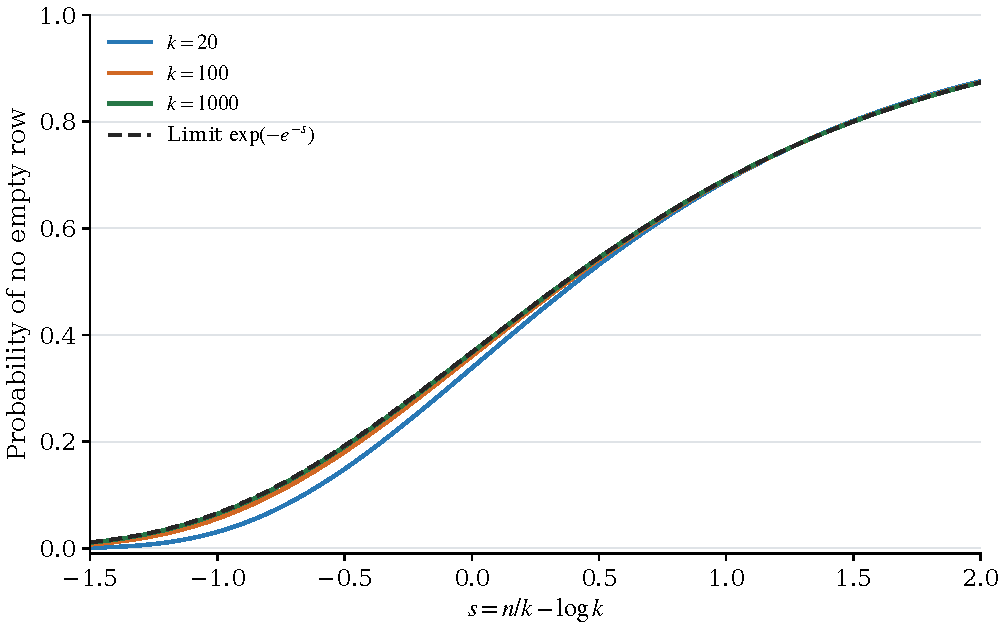
\includegraphics[width=0.92\textwidth]{figures/06-hankel-coupon_window.pdf}
\caption{The empty-row transition. Finite-height curves connect
evaluations at integer masses for $k=20,100,1000$; the dashed curve is
$\exp(-e^{-s})$. The horizontal coordinate always uses the actual
$s=n/k-\log k$. The probabilities are evaluated by the bounded
Bonferroni calculation described above.}
\label{mxc:fig:numeric-coverage}
\end{figure}

\subsection{The dense diagonal and two correction coefficients}
For A261784 define the normalized exact count
\[
 \mathcal R_N=\frac{T(2N,N)}{c_*d_*^N(N!)^2/N},
\]
with $c_*,d_*$ from~\eqref{mxc:eq:784-c} and~\eqref{mxc:eq:784-d}.
The all-orders expansion~\eqref{mxc:eq:dense-allorders}, specialized at
$\lambda=2$, gives
\[
 \mathcal R_N=1+\frac{\beta_1}{N}+\frac{\beta_2}{N^2}
                  +O(N^{-3}),\qquad \beta_1=\beta.
\]
There is an exact coefficient rule for the second constant:
\begin{equation}\label{mxc:eq:numeric-beta2}
 \beta_1=E_1(2)-\frac18,\qquad
 \beta_2=E_2(2)-\frac{E_1(2)}8+\frac1{128}.
\end{equation}
Here $E_1,E_2$ are obtained from the finite Gaussian-moment rule
\eqref{mxc:eq:saddle-algorithm}; the last two terms arise from the
central-binomial expansion. Evaluating that rule, independently of
the diagonal integer data, gives
\begin{align*}
 \beta_1&=-0.521806701556482663889144103069\ldots,\\
 \beta_2&=\phantom{-}0.128288828088705778459796704234\ldots.
\end{align*}
Thus $\beta_2$ is a derived coefficient rather than a fitted constant.
The finite arithmetic expression used for its evaluation is included
in \texttt{code/verify.py}.

To display the convergence, define
\[
 U_N=N(\mathcal R_N-1),\qquad
 V_N=N^2\left(\mathcal R_N-1-\frac{\beta_1}{N}\right),
\]
\[
 W_N=N^3\left(\mathcal R_N-1-\frac{\beta_1}{N}
                                -\frac{\beta_2}{N^2}\right).
\]
Theorem~\ref{mxc:thm:dense} and its all-orders refinement imply
$U_N\to\beta_1$, $V_N\to\beta_2$, and boundedness of $W_N$.
The numerator $T(2N,N)$ in every row of
Table~\ref{mxc:tab:numeric-diagonal} is computed as an exact integer from
\eqref{mxc:eq:stirling}; only the normalization uses floating arithmetic.

\begin{table}[htbp]
\centering\small
\begin{tabular}{@{}rrrr@{}}
\toprule
$N$ & $U_N$ & $V_N$ & $W_N$\\
\midrule
5   & $-0.49620219$ & $0.12802256$ & $-0.00133133$\\
10  & $-0.50899740$ & $0.12809304$ & $-0.00195793$\\
20  & $-0.51539780$ & $0.12817802$ & $-0.00221621$\\
30  & $-0.51753296$ & $0.12821232$ & $-0.00229519$\\
50  & $-0.51924187$ & $0.12824171$ & $-0.00235602$\\
75  & $-0.52009661$ & $0.12825702$ & $-0.00238568$\\
100 & $-0.52052405$ & $0.12826482$ & $-0.00240032$\\
\bottomrule
\end{tabular}
\caption{Dense-diagonal diagnostics from exact integer counts. The
first two columns approach the independently derived correction
coefficients; the final column records the next scaled remainder.}
\label{mxc:tab:numeric-diagonal}
\end{table}

At $N=100$, the signed relative error after including $\beta_1/N$
is $1.28938\times10^{-5}$; after also including $\beta_2/N^2$ it is
$-2.41288\times10^{-9}$. These are finite numerical comparisons,
not uniform error constants for the asymptotic theorem.

[Added 3 October 2026, batch 85B: manuscript~01's
Table~\ref{mxc:tp:tab:errors} reports the same comparisons with the
opposite sign convention, approximation divided by exact count minus one;
at $N=100$ it lists $-1.289\times10^{-5}$ and $+2.413\times10^{-9}$, the
same two numbers to first order. Its exact counts $a_N$, $N\le200$, come
from its own program.]

\subsection{Reproduction and data}
The package includes the complete \LaTeX{} source, compiled article,
both Python programs, their pinned dependencies, the figure in PDF
and PNG form, and CSV/JSON outputs. From the package root,
\texttt{python3 code/verify.py} regenerates the checks and tables;
\texttt{python3 code/make\_figures.py} regenerates the plot. The
\texttt{README.txt} gives the dependency and \LaTeX{} build commands.
The programs use no network access after their dependencies are
installed. The supplied run records report Python 3.12.14,
SymPy 1.14.0, mpmath 1.3.0, and matplotlib 3.10.8.

[Added 3 October 2026, batch 85B: in this report the compiled article is
a build of the merged text, not manuscript~06's delivered PDF, and the
names are those listed at the start of this section. Both programs write
unprefixed files under their output root, which defaults to the directory
above \texttt{code/}, and \texttt{06-hankel-make\_figures.py} imports its
sibling as \texttt{verify}; they must therefore be rerun on a copy with
the delivered names restored, as the report README describes, never in
the report directory. At the intake's rerun on a copy (Python 3.13.5)
\texttt{verify.py} passed in about 5\,s of Python time and the figure
program took about 74\,s, against the 0.3\,s and 2.3\,s of the delivered
README; the six CSV files were byte-identical, five JSON files equal apart
from line endings, and the PNG figure pixel-identical.]

\section{Further research: precise questions and useful next steps}\label{mxc:sec:questions}

The following are proposed research problems motivated by the results
above. They are not assertions that every formulation is open throughout
the literature. The source audit was narrower than that. Each question
identifies a statement not proved in this article and a concrete way in
which its resolution would extend the present results.

\begin{question}[A uniform approximation across the triangle]
Can one obtain relative asymptotics for $T(n,k)$ that remain valid from
the near-diagonal boundary $n-k=o(k)$ through the dense rays and into
the coverage window $n/k=\log k+O(1)$?
\end{question}

There are two distinct boundaries to resolve. As $n/k\downarrow1$, the
saddle $r$ tends to zero, the variance parameter $b$ tends to zero, and
the compact-set saddle proof no longer applies. At the endpoint,
$T(n,n)=\mathsf F_n$ exactly. As $n/k$ grows, the saddle escapes to
infinity and the kernel estimates must hold on expanding disks.
A useful first deliverable is a uniform formula for $n=k+\ell$ with
$\ell$ growing through the range where a fixed-defect expansion ceases
to be accurate. A second is a proved overlap region in which the
positive-transform saddle estimate and the empty-row probability
estimate agree, including their relative errors. Such a result would
turn the separate formulas in this article into a controlled asymptotic
description of a much larger part of A261781.

\begin{question}[Wider windows and higher coverage corrections]
For which explicit ranges of $s_k=n/k-\log k$ can the Poisson--Charlier
expansion of Section~\ref{mxc:sec:poisson} be extended, and can all its
correction polynomials be generated with a uniform summable remainder?
\end{question}

The theorem here keeps $\eta=k e^{-n/k}$ in a fixed compact subset of
$(0,\infty)$. If $\eta$ grows, the factorial-moment sums are concentrated
at growing indices, so the same fixed-disk argument does not directly
give a useful relative estimate for the small probability $M=0$.
If $\eta$ tends to zero, a different error scale is appropriate.
Expanding the exact ratios $c_{k-j}d_{k-j}^n/(c_kd_k^n)$ suggests a
constructive series in Poisson--Charlier polynomials, but the admissible
joint growth of $j$, $\eta$, and $h$ must be proved. A satisfactory result
would state both an explicit range and a remainder that remains smaller
than the probabilities or distances being approximated.

[Added 3 October 2026, batch 85B: for the single event $M=0$ and bounded
$s$, the second half of this question is answered by manuscript~01:
Theorem~\ref{mxc:tp:thm:couponall} gives every correction polynomial of
$\Pp(M=0)$ by a finite algorithm, with a uniform remainder
$O((1+h)^{J+1}/k^{J+1})$ after order $J$. The question stays open for
the whole law of $M$ (the generating function~\eqref{mxc:eq:pc-pgf} and
the probability-mass expansion beyond the first correction) and for
every window wider than bounded $s$.]

\begin{question}[Joint local limits and residual dependence]
Can the Gaussian--Poisson convergence in Section~\ref{mxc:sec:joint} be
strengthened to a joint local limit theorem with an explicit first
correction?
\end{question}

For example, one can ask for a uniform approximation to
$\Pp(C=c,M=m)$ for integer $c$ in a growing central range and $m$ in a
specified range, and for the corresponding law conditioned on $M=0$.
The present moment-generating-function proof establishes distributional
independence after normalization, but it does not control the Fourier
integral away from the origin. A local theorem requires both this
off-axis control and a lattice analysis. The first mixed correction
would quantify the small dependence that survives before taking the
limit, and would refine the order-one column-moment formulas on dense
rays. This is a natural setting in which to compare joint Edgeworth
and Poisson--Charlier expansions.

\begin{question}[Small column weights and equivalence of ensembles]
How does the coverage transition change when the column weight
$u=u_k$ tends to zero, and when does conditioning its weighted model on
$C=m$ preserve the corresponding asymptotic laws?
\end{question}

For any fixed $m$, conditioning on $C=m$ removes the factor $u^m$, so
the resulting distribution is exactly the prescribed-column model.
The analytic difficulty is making that conditioning asymptotically
uniform when its probability may be small. The weighted pole estimate
in Section~\ref{mxc:sec:uniform} is uniform on compact positive weight
intervals; it does not supply a uniform spectral gap as $u\downarrow0$.
The explicit critical parameter
$m\log(1+n/(km))$ and its shift at $m\asymp(\log k)^2$ provide testable
targets for a joint saddle analysis in $z$ and $u$. Extending the
prescribed-column theorem from $m=o(k)$ to comparable or larger column
counts is another concrete part of this problem.

\begin{question}[A combinatorial explanation of determinant positivity]
Is there a direct combinatorial model for the coefficients of
$H_{k,s}(u)$, or a sign-reversing involution proving the product in
Theorem~\ref{mxc:thm:hankel}?
\end{question}

The entries of the determinant count matrices, but the determinant
itself is a signed sum of products of such counts. Its coefficientwise
positivity is presently explained by spectral factorization. A direct
model would explain the factors $\binom{k}{j}^{j}$ and the powers of
$(1+u)^m-u^m$, and might expose refinements that the one-variable
spectrum does not reveal. The negative smaller minor exhibited in
Section~\ref{mxc:sec:hankel} rules out a blanket appeal to total positivity.
One should seek a model specific to these maximal minors, or a precise
classification of which other minors have a definite sign.

\begin{question}[Recurrences in finite characteristic]
What is the minimal eventual recurrence of the column $T(n,k)$ over
$\mathbb F_p$, and how does it depend on $k$ and the prime $p$?
\end{question}

Over characteristic zero every pole survives and all root sets are
disjoint. Reduction modulo a prime can merge roots, make multiplicities
inseparable, or cancel numerator and denominator factors. The determinant
product isolates the possible exceptional primes through binomial
coefficients, powers of $2$, and factors $2^m-1$. It therefore supplies
an arithmetic guide, but does not by itself classify the remaining
rank or the reduced rational function at each exceptional prime.
An exact classification could yield new divisibility and periodicity
statements for the triangle, with fast recurrence-based proofs suitable
for individual OEIS entries.

\begin{question}[The limiting distribution of determinant zeros]
After removing the factors at $u=0$ and $u=-1$, what is the limiting
zero-counting measure of $H_{k,s}(u)$ as $k\to\infty$?
\end{question}

Every remaining zero has real part $-1/2$ and is the image of a root
of unity under $\zeta\mapsto1/(\zeta-1)$. Its multiplicity is controlled
by the weighted gcd sum over pairs $1\le i<j\le k$. Determining the
normalized measure therefore reduces to a specific arithmetic counting
problem, rather than an unknown root-location problem. Useful targets
include an explicit density along the vertical line, tail estimates
for zeros with large imaginary part, and the contribution of roots
of small order. The answer should specify whether the zero measure is
normalized by the full degree or by the degree remaining after the
two exceptional factors are removed.

\begin{question}[Which column models have the same coverage law?]
Which replacements for the unrestricted column generating function
$(1-z)^{-k}-1$ retain the window $n=k(\log k+s)$, and which alter its
first correction or its scale?
\end{question}

Natural examples impose bounded entries, bounded column sums, or a
weight depending on column size. The row symmetry needed for exact
factorial moments may survive even when the root-of-unity spectrum does
not. One can aim for sufficient analytic conditions on the dominant
pole and its row-deletion ratios that imply a Poisson law, then identify
which derivatives determine the first correction. A theorem formulated
this way would separate properties special to matrix compositions from
properties shared by a wider class of symmetric occupancy models.

\subsection{A practical order of attack}

For a continuation in ProveIt, the most direct algebraic project is to
formalize the reduced denominator and its no-cancellation proof, followed
by the resultant and maximal Hankel determinant identities. These
statements are finite algebra and have explicit base conventions. They
provide a manageable route to a proof-assistant-checked contribution
without first formalizing saddle-point analysis.

[Added 3 October 2026, batch 85B: manuscript~01 names the same first
target (Section~\ref{mxc:tp:sec:future}). Nothing of either manuscript is
formalized; the only formal neighbour is the Lean Fubini generating
function cited in Section~\ref{mxc:sec:scope}, and this paragraph is a
proposal, not a plan of the repository.]

For analytic work, the highest-value next targets are the near-diagonal
boundary and a proved overlap with the coverage regime. The positive
Stirling transform avoids cancellation and gives an explicit starting
point in both cases. The small-weight problem is a second substantial
direction, because the prescribed-column result already identifies a
change of scale that a uniform two-variable theory must explain.
The computation scripts in the accompanying package can supply
regression examples for these projects, but every extension needs a
new proof of its claimed uniformity and error bounds.


\part{Finite spectra, uniform asymptotics, and two Poisson limits}
\label{mxc:tp:part}

\section{Provenance, scope and notation of Part II}\label{mxc:tp:sec:front}

[Added 3 October 2026, batch 85B.] Part~II was added in the write of
batch~85B. It is built from manuscript~01 of batch~85 and prints
everything that manuscript adds to Part~I. Where the two manuscripts prove
the same statement, the statement is printed once, in Part~I, with a
bracketed note naming manuscript~01's version; Table~\ref{mxc:tp:tab:routes}
lists those second routes. Everything in Part~II is written in Part~I's
letters (Table~\ref{mxc:tab:dictionary}).

\paragraph{Standing assumption: $u=1$.} Manuscript~01 never weights
columns. \emph{Every statement of Part~II is at column weight $u=1$}: its
$A(n,k)$, $T(n,k)$, $c_k$, $d_k$, $F_k(z;1)$ and $M$ are the unweighted
objects of Part~I, and its generating variable $\xi$ in
Section~\ref{mxc:tp:sec:defect} marks the Stirling defect, not columns.
No weighted analogue of a Part~II result is claimed. Several of its proofs
use $u=1$ explicitly: the residue $-a_k/(2k)$, the bound $a_k\ge\frac12$,
the Fubini pole at $L=\log2$ and the constants of
Section~\ref{mxc:tp:sec:couponall} are the $u=1$ values of Part~I's
$-a_{k,u}/((1+u)k)$, $a_{k,u}\ge b$, $L_u$ and $\mu_k(u)$, $d_k(u)$.

\subsection{The manuscript}
Manuscript~01 of batch~85 is the archive
\nolinkurl{OEIS_Matrix_Compositions_Research.zip} (wrapper directory
\nolinkurl{matrix_compositions_research/}, 26 files), which arrived in
commit \texttt{317c1ce2e} and was placed in this report by commit
\texttt{fa2f3e419}. Its article is titled \emph{Matrix compositions: finite
spectra, uniform asymptotics, and two Poisson limits}, subtitled
\emph{Proofs for OEIS A261781 and all-orders refinements for A261784}
(22~pages, dated 3~October 2026). Its title page and PDF metadata read
``Research report prepared for Vladimir Reshetnikov''; it names no author
and no tool. Its pin is the repository tree revision
\texttt{d68b65ea064084fb121df9bb431b21d086f7be81} (2026-10-03, 17:08), at
which it read the series-and-transseries overview
\path{Analysis/Transseries/docs/series-and-transseries/README.md} (blob
\texttt{7bdc83aeb}) as motivation for its inversion section; its indexed
searches for A261781 and A261784 returned nothing and exposed a different
revision, \texttt{ce37e13f4} \cite{proveit01}.

It was written without sight of manuscript~06, the source of Part~I, which
arrived thirteen minutes later in commit \texttt{345284ac8}. The two texts
share 0.7\,\% (01 in 06) and 0.5\,\% (06 in 01) of their word 8-grams,
almost all of them bibliography entries. Every number they share agrees:
the constants $r$, $b$, $v$, $d_*$, $c_*$, $\beta_1$, $\beta_2$ in about
seventy printed digits, computed by two independent programs, and the
coverage probabilities they both tabulate.

\paragraph{Status of manuscript~01, as delivered.} It is a proof-bearing
research report, not a Lean-certified or independently refereed
publication. The two OEIS conjecture labels were present in the entry it
inspected. The A261784 leading asymptotic was already posted; it is not
claimed as a new prediction, and the entry is not said to label it a
conjecture. Priority for the additional uniform results is not
established by its bounded literature search. It separates the
\emph{proof} of a statement from \emph{priority} for that statement, and
says that no uninspected repository theorem is assumed and no Lean
certification is inherited merely by association.

\subsection{What is new, and a correction}\label{mxc:tp:sec:novelty}
Manuscript~01's abstract says that it proves the two conjectures posted in
A261781, the recurrence order $k(k+1)/2$ of column $k$ and the limit
$d_{k+1}-d_k\to1/L$; its delivered README and its OEIS draft
(Section~\ref{mxc:tp:sec:oeis}) say the same. That claim is narrowed here.
\begin{itemize}
\item A homogeneous constant-coefficient recurrence of order
 $\binom{k+1}{2}$ for column $k$, with the product denominator
 $Q_{k,1}(z)=\prod_{j=1}^k(2(1-z)^j-1)$, is Proposition~25 of Munarini,
 Poneti and Rinaldi \cite{mpr2009} (printed page~16), published in 2009,
 eight years before the conjecture; their Remark~26 prints the cases of
 two and three rows, the first of which is manuscript~01's
 example~\eqref{mxc:eq:smallexamples}. Manuscript~01 cites Propositions~1,
 12, 13 and~29 of that paper, but not Proposition~25 or Remark~26. What
 it proves that is new is the \emph{minimality}: the product is the
 reduced denominator, so no eventual constant-coefficient recurrence of
 smaller order exists, even over $\mathbb C$. Manuscript~06 states this
 correctly (Section~\ref{mxc:sec:scope} and
 Remark~\ref{mxc:rem:minimal-sources}).
\item The limit $d_{k+1}-d_k\to1/L$ is immediate from the closed form of
 \cite[Proposition~13]{mpr2009}, as both manuscripts say. Manuscript~01's
 genuine strengthening is that the increments \emph{increase strictly}
 and stay below $1/L$ (Theorem~\ref{mxc:tp:thm:monotone}).
\item Manuscript~01 says that Louchard's paper \cite{louchard} was
 identified through A261780 but not retrieved. That remains a true
 statement about its own preparation and its non-claim stands; but the
 paper is retrievable, and manuscript~06 inspected the author's long
 version and found no matching coverage-window statement
 (Section~\ref{mxc:sec:scope}). The intake confirmed that the author's
 publication list carries it as item~99 but did not read it.
\end{itemize}
The generating functions and the positive Stirling--Fubini transform are
Munarini, Poneti and Rinaldi's, and both manuscripts credit them; the
leading A261784 law, $d_*$ and the decimal value of $c_*$ are
Kot\v{e}\v{s}ovec's \cite{oeis784}.

New in manuscript~01 relative to manuscript~06, and printed below: strict
monotonicity of the increments (Section~\ref{mxc:tp:sec:monotone}); every
fixed order of the coverage probability
(Section~\ref{mxc:tp:sec:couponall}); the entire Stirling kernel with its
differential recurrence, its third polynomial and a second exact
algorithm (Section~\ref{mxc:tp:sec:kernel}); a recursion for the
cumulants (Section~\ref{mxc:tp:sec:saddle}); the Poisson law of the
Stirling defect (Section~\ref{mxc:tp:sec:defect}); the third diagonal
correction and fifty-digit constants (Section~\ref{mxc:tp:sec:diagonal});
an asymptotic inversion with integer threshold brackets, which is an
instance of the repository's inversion apparatus
(Section~\ref{mxc:tp:sec:inverse}); exact-ratio coverage and defect tables
(Sections~\ref{mxc:tp:sec:defect} and~\ref{mxc:tp:sec:checks}); and its
research questions and proof audit
(Sections~\ref{mxc:tp:sec:future}--\ref{mxc:tp:sec:oeis}).

\subsection{Manuscript 01's second routes to Part I's results}

\begin{table}[htbp]
\centering\small
\renewcommand{\arraystretch}{1.12}
\begin{tabular}{@{}>{\raggedright\arraybackslash}p{.28\textwidth}>{\raggedright\arraybackslash}p{.65\textwidth}@{}}
\toprule
Part I & Manuscript~01's version and route\\
\midrule
\eqref{mxc:eq:gf}--\eqref{mxc:eq:ie}, \eqref{mxc:eq:stirling} &
the same classical identities at $u=1$, credited to
\cite{mpr2009}; the Stirling transform proved by the same geometric
expansion and finite difference\\
Theorem~\ref{mxc:thm:minimal} &
the same theorem at $u=1$, same proof
(Remark~\ref{mxc:rem:minimal-sources}); the recurrence written from
$n>D$\\
\eqref{mxc:eq:fixedk}, Corollary~\ref{mxc:cor:increment} &
the same constants and expansions of $d_k$, $c_k$; adds strict
monotonicity (Theorem~\ref{mxc:tp:thm:monotone}); lacks
\eqref{mxc:eq:d-incr}\\
Theorem~\ref{mxc:thm:uniform} &
the bound $(k-1)\rho^{n+1}$, $u=1$ only
(Remark~\ref{mxc:rem:uniform-ms01})\\
\eqref{mxc:eq:pc-zero}, Corollary~\ref{mxc:cor:coverage} &
the same expansion of $\Pp(M=0)$ and Poisson limit, by Bonferroni
truncation of inclusion--exclusion (note after
Theorem~\ref{mxc:thm:pc-pgf}); no generating function in complex $w$, no
probability-mass or total-variation statement\\
\eqref{mxc:eq:fubini-estimate} & the same lemma, same proof\\
\eqref{mxc:eq:dense-reduction}, Lemma~\ref{mxc:lem:kernel} &
the untruncated kernel $\mathsf W_n$, with no hypothesis on $k$
(Remark~\ref{mxc:rem:kernel-untruncated},
Section~\ref{mxc:tp:sec:kernel})\\
Theorem~\ref{mxc:thm:dense}, \eqref{mxc:eq:saddle-algorithm},
\eqref{mxc:eq:dense-allorders} &
the same theorem and prescription; tails by $|\mathsf W_n(w)|\le e^{|w|}$
(notes after the proof of Theorem~\ref{mxc:thm:dense} and
after~\eqref{mxc:eq:dense-allorders})\\
Corollary~\ref{mxc:cor:784}, \eqref{mxc:eq:numeric-beta2} &
the same constants and $\beta_1$, $\beta_2$; adds $\beta_3$ and all orders
(Section~\ref{mxc:tp:sec:diagonal})\\
$\E D$, $\Var D$ in Corollary~\ref{mxc:cor:dense-columns} &
implied by the Poisson law of $\Delta_{n,k}=D$
(Theorem~\ref{mxc:tp:thm:defect})\\
Table~\ref{mxc:tab:numeric-coverage}, Table~\ref{mxc:tab:numeric-diagonal} &
Tables~\ref{mxc:tp:tab:coupon} and~\ref{mxc:tp:tab:errors}, from its own
exact counts; equal where they overlap\\
\bottomrule
\end{tabular}
\caption{Results of Part~I that manuscript~01 proves as well, and its
version of each. None is reprinted in Part~II.}
\label{mxc:tp:tab:routes}
\end{table}

Results of Part~I that manuscript~01 does not have: the column weight $u$
throughout; the initial impulse (Remark~\ref{mxc:rem:impulse}); the whole
Hankel section (Theorem~\ref{mxc:thm:hankel}); the uniform constant of
Theorem~\ref{mxc:thm:uniform}; the coverage generating function, the
probability-mass and total-variation expansions and the moving-mean
remark of Section~\ref{mxc:sec:poisson}; the joint Gaussian--Poisson law
of Section~\ref{mxc:sec:joint}; the column central limit theorem on dense
rays (Corollary~\ref{mxc:cor:dense-columns}); and the prescribed-column
threshold of Section~\ref{mxc:sec:fixedcolumns}.

\section{Strict monotonicity of the growth-constant increments}\label{mxc:tp:sec:monotone}

Extend $d_k$ to real $x>0$ by $d(x)=(1-2^{-1/x})^{-1}$, so that
$d_k=d(k)$.

\begin{theorem}[Strengthened increment statement]\label{mxc:tp:thm:monotone}
The sequence $d_{k+1}-d_k$, $k\ge1$, is strictly increasing, is always
below $1/L$, and tends to $1/L$.
\end{theorem}
\begin{proof}
Put $t=L/(2x)$. Since $d(x)=\frac12+\frac12\coth t$,
\begin{equation}\label{mxc:tp:eq:dprime}
 d'(x)=\frac1L\left(\frac{t}{\sinh t}\right)^2.
\end{equation}
This lies strictly between $0$ and $1/L$. The function $t/\sinh t$ is
strictly decreasing for $t>0$, because $\sinh t-t\cosh t<0$; the latter
expression vanishes at $0$ and has derivative $-t\sinh t<0$. As $x$
increases, $t$ decreases; thus $d'$ increases strictly to $1/L$.
Integrating $d'$ over $[k,k+1]$ proves the claim.
\end{proof}

\begin{remark}[Further details from manuscript~01]\label{mxc:tp:rem:details}
(i)~The inverse of~\eqref{mxc:eq:ie} is
$A(n,k)=\sum_{j=0}^k\binom kjT(n,j)$: choose the nonzero rows. Also
$T(n,k)=0$ for $k>n$, and the rational expression~\eqref{mxc:eq:gf} at
$u=1$ equals $1$ for $k=0$, as it must. (ii)~The bijection with the
sorted-word compositions of A261780 and A261781 lists the row label $i$
as many times as the entry in row~$i$ of a column, in increasing order;
column boundaries become part boundaries, and the construction is
reversible. (iii)~At the unique smallest-modulus pole $1-a_k$ only the
$j=k$ summand of~\eqref{mxc:eq:ie} contributes, with residue $-a_k/(2k)$,
so its coefficient contribution is
$\frac{a_k}{2k}(1-a_k)^{-n-1}=c_kd_k^n$. (iv)~The alternating
sum~\eqref{mxc:eq:ie} explains why cancellation is a numerical concern
when all rows must be occupied; the positive
transform~\eqref{mxc:eq:stirling} is an exact computational alternative
to it.
\end{remark}

\section{Every fixed order in the coverage window}\label{mxc:tp:sec:couponall}

For real $x\to\infty$ the exact constants have the expansions
\begin{align}
 \log d(x)&=\log\frac xL+\frac{L}{2x}-\frac{L^2}{24x^2}+O(x^{-4}),
 \label{mxc:tp:eq:logd}\\
 \log c(x)&=-\log(2L)-\frac{L}{2x}-\frac{L^2}{24x^2}+O(x^{-4}),
 \label{mxc:tp:eq:logc}
\end{align}
where $c(x)=(d(x)-1)/(2x)$; these are the identities for $\log d_m$ and
$\log c_m$ in the proof of Theorem~\ref{mxc:thm:pc-pgf}, with
$g_0(x)=-L^2x^2/24+O(x^4)$, and both differences from the leading
logarithms are analytic in $1/x$ at $0$. Let $\mathcal T_a(x)$ denote the
Touchard polynomial, defined by
$\sum_{j\ge0}j^ax^j/j!=e^x\mathcal T_a(x)$.

\begin{theorem}[All fixed orders for coverage]\label{mxc:tp:thm:couponall}
Let $k\to\infty$ through integers, with $h=n/k=\log k+s$ and
$\eta=ke^{-h}=e^{-s}$, where $s$ stays in a fixed compact real interval.
For every fixed $J\ge0$ there are polynomials
$\mathcal Q_1,\ldots,\mathcal Q_J$ in $h$ and $\eta$, with coefficients
polynomial in $L$ over $\mathbb Q$, such that
\begin{equation}\label{mxc:tp:eq:couponall}
 \frac{T(n,k)}{A(n,k)}=\Pp(M=0)=e^{-\eta}
 \left[1+\sum_{j=1}^{J}\frac{\mathcal Q_j(h,\eta;L)}{k^j}
 +O\!\left(\frac{(1+h)^{J+1}}{k^{J+1}}\right)\right],
\end{equation}
uniformly in such $s$. Each $\mathcal Q_j$ has degree at most $j$ in
$h$, and
\[
 \mathcal Q_1(h,\eta;L)=\tfrac12\bigl((1-L)h\eta-(h+1)\eta^2\bigr).
\]
\end{theorem}
For $J=1$ this is~\eqref{mxc:eq:pc-zero}.

\begin{proof}
Put $\epsilon=1/k$ (a local letter; Part~I's $\epsilon$ in
Section~\ref{mxc:sec:allorders} is $1/n$). Using the analytic expansions
behind \eqref{mxc:tp:eq:logd}--\eqref{mxc:tp:eq:logc}, form the formal power
series in $\epsilon$
\begin{equation}\label{mxc:tp:eq:couponalgorithm}
 \Psi(j,h,\epsilon)=\sum_{i=0}^{j-1}\log(1-i\epsilon)
 +\log\frac{c(\epsilon^{-1}-j)}{c(\epsilon^{-1})}
 +\frac h\epsilon\left(\log\frac{d(\epsilon^{-1}-j)}{d(\epsilon^{-1})}
                 +j\epsilon\right).
\end{equation}
By~\eqref{mxc:eq:pc-moments} and Theorem~\ref{mxc:thm:uniform},
$\E(M)_j=\eta^j\exp\Psi(j,h,1/k)$ up to the exponentially small spectral
errors. The cancellation in the last parentheses removes its linear
leading term. Every coefficient of $\Psi$ is a polynomial in $j$, $h$,
$L$, and its dependence on $h$ is at most linear. Hence
$[\epsilon^i]e^\Psi$ is a polynomial in $j$, $h$, $L$ of degree at most
$i$ in $h$. Replace each monomial $j^a$ in that coefficient by
$\mathcal T_a(-\eta)$ to obtain $\mathcal Q_i$; this is the summation
$\sum_j(-\eta)^jj^a/j!=e^{-\eta}\mathcal T_a(-\eta)$ of the
inclusion--exclusion series $\Pp(M=0)=\sum_j(-1)^j\E(M)_j/j!$.

To justify the operation, truncate at $j\le C\log k$. Taylor's formula
applied to the finitely many logarithms and to
\eqref{mxc:tp:eq:logd}--\eqref{mxc:tp:eq:logc}, continued to the required
order, bounds the moment remainder by
\[
 \frac{\eta^j}{k^{J+1}}C_J(1+h)^{J+1}(1+j)^{C'_J}
\]
for constants $C_J$, $C'_J$ on the chosen $s$-interval. The exponential of
the small discarded logarithm is uniformly bounded in this range. Summing
against $1/j!$ preserves the stated error, and the Bonferroni
inequalities bound the tail superalgebraically, as in the second route
noted after Theorem~\ref{mxc:thm:pc-pgf}. This proves both the algorithm and
the uniform remainder.
\end{proof}

The appearance of $\log k$ inside the coefficients, through $h$, is
intrinsic to the transition scale. Theorem~\ref{mxc:tp:thm:couponall} is an
all-orders Poincar\'e expansion of the single probability $\Pp(M=0)$; it
does not assert convergence as $J\to\infty$, nor a classification of
exponentially small terms, and it does not extend Part~I's expansion of
the whole law of $M$ beyond the first correction (see the note to
Research question~2 in Section~\ref{mxc:sec:questions}).

\section{The entire Stirling kernel}\label{mxc:tp:sec:kernel}

For $n\ge1$ define, with the falling factorial $(n)_\ell$ of Part~I and
$(n)_0=1$,
\begin{equation}\label{mxc:tp:eq:kerneldef}
 \chi_{n,\ell}=\frac{\StirOne{n}{n-\ell}}{(n)_\ell^{\,2}},\qquad
 \mathsf W_n(w)=\sum_{\ell=0}^{n-1}\chi_{n,\ell}w^\ell,
\end{equation}
and set $\chi_{n,\ell}=0$ outside $0\le\ell<n$. By
Remark~\ref{mxc:rem:kernel-untruncated}, Part~I's kernel is the truncation
$H_{n,k}(z)=\sum_{\ell\le n-k}\chi_{n,\ell}(Lz)^\ell$.

\begin{proposition}[Positive coefficient representation]\label{mxc:tp:prop:kernelrep}
Let $f(z)=e^z-1$ and
\begin{equation}\label{mxc:tp:eq:Ttilde}
 \widetilde T(n,k)=\frac{n!}{2L^{n+1}}[z^n]f(z)^k\mathsf W_n(Lz).
\end{equation}
For $n\ge k\ge1$, $T(n,k)=\widetilde T(n,k)(1+O_\vartheta(\vartheta^k))$.
\end{proposition}
\begin{proof}
In~\eqref{mxc:eq:stirling} replace $\mathsf F_q$
using~\eqref{mxc:eq:fubini-estimate}, use
$\StirTwo qk=q![z^q]f(z)^k/k!$ and put $q=n-\ell$. The resulting exact
main sum is
\[
 \frac{1}{2\,n!\,L^{n+1}}\sum_{\ell=0}^{n-1}\StirOne{n}{n-\ell}
 ((n-\ell)!)^2L^\ell[z^{n-\ell}]f(z)^k,
\]
which is~\eqref{mxc:tp:eq:Ttilde}. Positivity of every summand transports
the relative error.
\end{proof}

\begin{lemma}[Bounds and an exact differential recurrence]\label{mxc:tp:lem:kernelbound}
For $0\le\ell<n$, $0\le\chi_{n,\ell}\le1/\ell!$; consequently
$|\mathsf W_n(w)|\le e^{|w|}$ for every complex $w$. With
$D_w=w\,\mathrm d/\mathrm dw$,
\begin{equation}\label{mxc:tp:eq:kernelrec}
 (n+1)^2\mathsf W_{n+1}(w)=\bigl((n+1-D_w)^2+nw\bigr)\mathsf W_n(w),
 \qquad \mathsf W_1(w)=1.
\end{equation}
\end{lemma}
\begin{proof}
The first-kind coefficient $\StirOne{n}{n-\ell}$ is the $\ell$th
elementary symmetric polynomial of $1,2,\ldots,n-1$. Each of its
$\binom{n-1}{\ell}$ summands is at most $(n-1)_\ell$. Hence
\[
 \chi_{n,\ell}\le\frac{(n-1)_\ell^{\,2}}{\ell!\,(n)_\ell^{\,2}}\le\frac1{\ell!}.
\]
The first-kind recurrence gives
\[
 \chi_{n+1,\ell}=\frac{(n+1-\ell)^2}{(n+1)^2}\chi_{n,\ell}
 +\frac{n}{(n+1)^2}\chi_{n,\ell-1}.
\]
Multiplying by $w^\ell$ and summing proves~\eqref{mxc:tp:eq:kernelrec}.
\end{proof}

\begin{theorem}[Uniform entire kernel expansion]\label{mxc:tp:thm:kernel}
For each fixed $J\ge0$ there are rational polynomials $P_0,\ldots,P_J$,
with $P_0=1$ and $\deg P_r\le2r$, such that
\begin{equation}\label{mxc:tp:eq:kernelall}
 \mathsf W_n(w)=e^{w/2}\left(\sum_{r=0}^{J}\frac{P_r(w)}{n^r}
 +O_{J,K}(n^{-J-1})\right)
\end{equation}
uniformly on every compact $K\subset\mathbb C$, with no condition
relating $n$ to any $k$. The expansion may be differentiated any fixed
number of times, uniformly on compact sets. The polynomials are those of
\eqref{mxc:eq:kernel-allorders}:
\begin{align}
 P_1(w)&=\frac{w^2}{12}-\frac w2,\qquad
 P_2(w)=\frac{w^4}{288}-\frac{w^2}{12},\notag\\
 P_3(w)&=\frac{w^6}{10368}+\frac{w^5}{576}+\frac{w^4}{480}
 -\frac{w^3}{24}-\frac{w^2}{12}.\label{mxc:tp:eq:p3}
\end{align}
\end{theorem}

\begin{proof}
This is a coefficient-level proof with a uniform remainder. Let
$\Sigma_j(n)=\sum_{a=1}^{n-1}a^j$, regarded as its Faulhaber polynomial in
$n$. With $\epsilon=1/n$ put $\mathsf a_j(\epsilon)=\epsilon^{2j}\Sigma_j(1/\epsilon)$.
This is a polynomial beginning in degree $j-1$, and
$\mathsf a_1(\epsilon)=(1-\epsilon)/2$. For a fixed integer $\ell\ge0$
define
\begin{equation}\label{mxc:tp:eq:analyticR}
 \mathsf e_\ell(\epsilon)=[t^\ell]\exp\left(
 \sum_{j=1}^{\ell}\frac{(-1)^{j-1}}{j}\mathsf a_j(\epsilon)t^j\right),
 \qquad
 \mathsf r_\ell(\epsilon)=\mathsf e_\ell(\epsilon)
 \prod_{a=0}^{\ell-1}(1-a\epsilon)^{-2}.
\end{equation}
Newton's identity for elementary symmetric functions shows that
$\mathsf r_\ell(1/n)=\chi_{n,\ell}$ whenever $n>\ell$. In particular
$\mathsf r_\ell(0)=1/(2^\ell\ell!)$.

The exponent in~\eqref{mxc:tp:eq:analyticR} is
$t/2+\sum_{r\ge1}\epsilon^r\mathsf b_r(t)$ with $\deg\mathsf b_r\le r+1$.
Thus at total order $\epsilon^r$ the part multiplying $e^{t/2}$ has
degree at most $2r$ in $t$, and extracting $t^\ell$ converts
$t^qe^{t/2}$ into $2^q(\ell)_q/(2^\ell\ell!)$. The other factor of
$\mathsf r_\ell$ has logarithm
$2\sum_{r\ge1}\frac{\epsilon^r}{r}\sum_{a=0}^{\ell-1}a^r$, whose
coefficient at order $r$ is a polynomial in $\ell$ of degree
$r+1\le2r$. Therefore
\begin{equation}\label{mxc:tp:eq:Pr}
 [\epsilon^r]\mathsf r_\ell(\epsilon)=\frac{\Pi_r(\ell)}{2^\ell\ell!},
 \qquad \Pi_r\in\mathbb Q[\ell],\quad\deg\Pi_r\le2r;
\end{equation}
for example $\Pi_0=1$ and $\Pi_1(\ell)=\ell(\ell-4)/3$, the polynomial
$d(d-4)/3$ of the proof of Lemma~\ref{mxc:lem:kernel}.

Next, the Taylor remainders are bounded uniformly in $\ell$. There are
absolute $c,C>0$ such that, for $|\epsilon|\le c/(\ell+1)^2$ and
$2\le j\le\ell$,
\begin{equation}\label{mxc:tp:eq:faulbound}
 |\mathsf a_j(\epsilon)|\le C|\epsilon|^{j-1}.
\end{equation}
For completeness: Faulhaber's formula writes $\mathsf a_j$ as
$\frac1{j+1}\sum_{a=0}^j\binom{j+1}{a}\mathbf B_a\epsilon^{j-1+a}$, with
Bernoulli numbers $\mathbf B_a$. The coefficients of $t/(e^t-1)$ obey
$|\mathbf B_a|/a!\le C_0$ by a Cauchy bound on a fixed circle of
radius~$1$. Since $j!/(j+1-a)!\le j^{a-1}$ for $a\ge1$, the sum of the
terms after the first is bounded by a geometric series in $j|\epsilon|$.

For $\ell\ge1$, apply Cauchy's coefficient bound
in~\eqref{mxc:tp:eq:analyticR} on $|t|=2\ell$. The $j=1$ term contributes at
most $\ell+O(1)$ to the real part of the exponent, while
\eqref{mxc:tp:eq:faulbound} bounds the sum of the terms $j\ge2$ by a
constant, because $|\epsilon|\ell^2$ is bounded; the product
$\prod(1-a\epsilon)^{-2}$ is bounded for the same reason. Stirling's
factorial estimate then gives
\begin{equation}\label{mxc:tp:eq:Rbound}
 \sup_{|\epsilon|\le c/(\ell+1)^2}|\mathsf r_\ell(\epsilon)|
 \le\frac{C\sqrt{\ell+1}}{2^\ell\ell!};
\end{equation}
for $\ell=0$ this is immediate. Cauchy's Taylor-remainder estimate at
$\epsilon=1/n$ consequently yields
\begin{equation}\label{mxc:tp:eq:kerneluniformcoeff}
 \chi_{n,\ell}=\frac1{2^\ell\ell!}\sum_{r=0}^{J}\frac{\Pi_r(\ell)}{n^r}
 +O_J\!\left(\frac{(\ell+1)^{2J+5/2}}{2^\ell\ell!\,n^{J+1}}\right)
\end{equation}
whenever $\ell\le\delta_0\sqrt n$, for a sufficiently small absolute
$\delta_0>0$ and all sufficiently large $n$.

Multiply~\eqref{mxc:tp:eq:kerneluniformcoeff} by $w^\ell$ and sum. On
$|w|\le V$ the remainder is summable uniformly. Beyond $\delta_0\sqrt n$
the bound $\chi_{n,\ell}\le1/\ell!$ makes the original tail smaller than
every power of $n^{-1}$, and the same holds for the polynomially weighted
Taylor coefficients in~\eqref{mxc:tp:eq:Pr}. Hence
\[
 \mathsf W_n(w)=\sum_{r=0}^{J}\frac1{n^r}\sum_{\ell\ge0}
 \frac{\Pi_r(\ell)}{\ell!}\Bigl(\frac w2\Bigr)^\ell+O_{J,V}(n^{-J-1}).
\]
The inner sum is $e^{w/2}$ times a polynomial of degree at most $2r$, by
the Touchard identity. This proves~\eqref{mxc:tp:eq:kernelall}; expanding
\eqref{mxc:tp:eq:analyticR} gives $P_1$, $P_2$, $P_3$. Cauchy's derivative
estimate on a slightly larger compact disk gives the differentiated
expansions.
\end{proof}

\paragraph{A finite exact coefficient algorithm.} The polynomials can be
computed without a symbolic parameter $\ell$. For a requested order $J$,
compute $e_\ell(n)=\StirOne{n}{n-\ell}$ for $0\le\ell\le2J$ by
\begin{equation}\label{mxc:tp:eq:newtonalgorithm}
 e_0(n)=1,\qquad
 \ell e_\ell(n)=\sum_{j=1}^{\ell}(-1)^{j-1}e_{\ell-j}(n)\Sigma_j(n),
\end{equation}
expand $e_\ell(n)/(n)_\ell^2$ in powers of $1/n$ to order $J$, and use
$\deg P_r\le2r$:
\begin{equation}\label{mxc:tp:eq:pkernelalgorithm}
 P_r(w)=\sum_{m=0}^{2r}w^m\sum_{\ell=0}^{m}
 \frac{(-1/2)^{m-\ell}}{(m-\ell)!}\,
 [n^{-r}]\frac{e_\ell(n)}{(n)_\ell^{\,2}}.
\end{equation}
Here $[n^{-r}]$ is the coefficient in the expansion at infinity, not a
coefficient of the polynomial numerator alone. Manuscript~01's program
(\path{code/01-two-poisson-verify.py}) runs
\eqref{mxc:tp:eq:newtonalgorithm}--\eqref{mxc:tp:eq:pkernelalgorithm} exactly
over $\mathbb Q$ and checks~\eqref{mxc:tp:eq:kernelrec} coefficientwise
through $n=80$. This is a second finite route to Part~I's
algorithm~\eqref{mxc:eq:R-algorithm}--\eqref{mxc:eq:P-algorithm}.
[Added 3 October 2026, batch 85B: the intake checked $P_3$ numerically:
at $w=1.3$, $n^3\bigl(e^{-w/2}\mathsf W_n(w)-1-P_1/n-P_2/n^2\bigr)$ is
$-0.22070$, $-0.22010$, $-0.21981$ for $n=400$, $800$, $1600$, against
$P_3(1.3)=-0.21951$, with the expected $O(1/n)$ approach.]

\section{Complements on compact rays}\label{mxc:tp:sec:saddle}

Manuscript~01 writes the leading factor of Theorem~\ref{mxc:thm:dense} as
\begin{equation}\label{mxc:tp:eq:Bnk}
 \mathcal B(n,k)=\frac{n!\,f(r)^ke^{v}}{2L^{n+1}r^n\sqrt{2\pi kb}},
 \qquad
 T(n,k)=\mathcal B(n,k)\Bigl[1+\sum_{j=1}^J\frac{E_j(\lambda)}{k^j}
 +O_{J,K}(k^{-J-1})\Bigr].
\end{equation}
It adds two observations and a recursion.

\paragraph{The variance $b$.} $b=\kappa_2=\lambda(1+r-\lambda)$ is the
variance of the positive-integer random variable with probabilities
proportional to $r^j/j!$, $j\ge1$, which explains its positivity; the
proof needs only the monotonicity of $r/(1-e^{-r})$.

\paragraph{A recursion for the cumulants.} With independent variables
$z$, $a$, define
\begin{equation}\label{mxc:tp:eq:cumulantalgorithm}
 \mathcal K_1(z,a)=a,\qquad
 \mathcal K_{j+1}=z\,\partial_z\mathcal K_j+a(1+z-a)\,\partial_a\mathcal K_j.
\end{equation}
Then $\kappa_j=\mathcal K_j(r,\lambda)$. This follows from
$\mathcal D\lambda=\lambda(1+z-\lambda)$ for
$\lambda(z)=\mathcal D\log f(z)=z/(1-e^{-z})$, before evaluation at the
saddle. One must not differentiate a specialized formula while holding
$\lambda$ fixed. (For example
$\mathcal K_3=a\bigl(2a^2-3az-3a+z^2+3z+1\bigr)$, which is the expanded
$\kappa_3$ printed after Theorem~\ref{mxc:thm:dense}.) Together with
\eqref{mxc:tp:eq:pkernelalgorithm} and~\eqref{mxc:eq:saddle-algorithm},
this specifies every $E_j$ by finite rational operations and the
evaluation of $r$; in fact $E_j$ is a rational function of $r$,
$\lambda$, $L$ whose denominators are powers of $b$ and $\lambda$.

\begin{remark}[Floors and endpoints]\label{mxc:tp:rem:floors}
The ratio in Theorem~\ref{mxc:thm:dense} is the \emph{actual} $n/k$. For
$n=\lfloor\lambda_0k\rfloor$, replacing it prematurely by $\lambda_0$
inside exponential factors can lose a nonvanishing factor. The theorem is
not uniform as $\lambda\downarrow1$ or $\lambda\to\infty$; at the
boundary $n=k$ the exact identity is $T(n,n)=\mathsf F_n$, and the
coverage window, where $\lambda\sim\log k$, needs the separate proof of
Section~\ref{mxc:sec:poisson}. Manuscript~01's optional program
\path{code/01-two-poisson-ray_spotchecks.py} tests the expansion at
$\lambda=3/2$, $3$ and $5$ for $40\le k\le200$ with 75-digit arithmetic
(\path{data/01-two-poisson-ray_spot_checks.csv}); the relative error after
the third correction is between $2.38\times10^{-12}$ and
$1.63\times10^{-9}$ in absolute value at the seven tested points.
\end{remark}

\section{The Stirling defect: a second Poisson limit}\label{mxc:tp:sec:defect}

The positive identity~\eqref{mxc:eq:stirling} supplies an auxiliary
probability space. It should not be confused with the zero-row
statistic $M$, which vanishes identically on the objects counted by $T$.

\begin{definition}\label{mxc:tp:def:defect}
For $n\ge k\ge1$, define $Q_{n,k}$ on $\{k,\ldots,n\}$ by
\begin{equation}\label{mxc:tp:eq:defectdef}
 \Pp(Q_{n,k}=q)=\frac{\StirOne nq\StirTwo qk\mathsf F_q}
 {\sum_{p=k}^n\StirOne np\StirTwo pk\mathsf F_p},
 \qquad \Delta_{n,k}=n-Q_{n,k}.
\end{equation}
$\Delta_{n,k}$ is the \emph{Stirling defect} of the transform. $Q_{n,k}$
and $\Delta_{n,k}$ are Part~I's $Q$ and $D$ of
Section~\ref{mxc:sec:dense-columns}.
\end{definition}

\begin{theorem}[Poisson defect and analytic generating functions]\label{mxc:tp:thm:defect}
Suppose $n,k\to\infty$ and $n/k\to\lambda_0\in(1,\infty)$. Then
\begin{equation}\label{mxc:tp:eq:defectlimit}
 \Delta_{n,k}\xrightarrow{\mathrm d}\Pois\!\Bigl(\frac{Lr(\lambda_0)}2\Bigr).
\end{equation}
More precisely, uniformly for complex $\xi$ in compact sets and for $n/k$
in compact subsets of $(1,\infty)$,
\begin{equation}\label{mxc:tp:eq:defectpgf}
 \E\xi^{\Delta_{n,k}}=e^{v(\xi-1)}\bigl(1+O(k^{-1})\bigr),
 \qquad v=\frac{Lr(n/k)}2.
\end{equation}
There is an expansion through every fixed order, locally uniformly in
$\xi$, and the same holds for each fixed derivative with respect to
$\xi$.
\end{theorem}
\begin{proof}
Marking $n-q=\ell$ in the main transform replaces $\mathsf W_n(Lz)$ by
$\mathsf W_n(\xi Lz)$. Lemma~\ref{mxc:tp:lem:kernelbound} and positivity
bound the Fubini replacement error, also for bounded complex $\xi$ by
using absolute values. The proof of Theorem~\ref{mxc:thm:dense}, with $\xi$
in a compact set, now replaces $e^{Lr/2}$ by $e^{\xi Lr/2}$; this uses
Theorem~\ref{mxc:tp:thm:kernel} on compact sets of $\mathbb C$. Division by
the unmarked coefficient gives~\eqref{mxc:tp:eq:defectpgf}; the
denominator's leading factor is positive and bounded away from zero after
normalization, so the division is uniform. Replacing $P_p(Lre^{\tau y})$
by $P_p(\xi Lre^{\tau y})$ in~\eqref{mxc:eq:saddle-algorithm} gives every
higher order. Uniform holomorphy on a larger compact set permits
differentiation. Coefficient extraction at $\xi=0$ yields convergence of
each probability to the corresponding Poisson mass, and these limiting
masses sum to one.
\end{proof}

Differentiating~\eqref{mxc:tp:eq:defectpgf} once and twice at $\xi=1$ gives
$\E\Delta_{n,k}=v+O(k^{-1})$ and $\Var\Delta_{n,k}=v+O(k^{-1})$, the two
moments of Corollary~\ref{mxc:cor:dense-columns}. The theorem explains
why only a bounded distance below the top Stirling index contributes at
leading order, although the positive sum ranges from $k$ to $n$: the
factor $e^{v}=e^{Lr/2}$ in~\eqref{mxc:tp:eq:Bnk} is exactly the aggregate
contribution of the limiting Poisson cloud. The report does not assert
that $\Delta_{n,k}$ is a canonical statistic on unadorned matrices;
finding such a statistic is a separate combinatorial problem
(Section~\ref{mxc:tp:sec:future}).

For $n=2N$, $k=N$ the limiting mean is $v=0.55230808135934145323\ldots$.
Direct evaluation of the positive weights in~\eqref{mxc:tp:eq:defectdef}
gives Table~\ref{mxc:tp:tab:defect}.
\begin{table}[htbp]
\centering\small
\begin{tabular}{@{}rrrrr@{}}
\toprule
$\ell$ & $N=10$ & $N=50$ & $N=200$ & $e^{-v}v^\ell/\ell!$\\
\midrule
\tableinput{data/01-two-poisson-defect_table.tex}
\bottomrule
\end{tabular}
\caption{Convergence of $\Pp(\Delta_{2N,N}=\ell)$ to its Poisson limit
(manuscript~01).}
\label{mxc:tp:tab:defect}
\end{table}

\section{A261784: the third correction and every further one}\label{mxc:tp:sec:diagonal}

\begin{corollary}[Diagonal expansion to every order]\label{mxc:tp:cor:diagonal}
For every fixed $J\ge0$,
\begin{equation}\label{mxc:tp:eq:diagonalall}
 a_N=c_*d_*^N\frac{(N!)^2}{N}
 \left(1+\sum_{j=1}^{J}\frac{\beta_j}{N^j}+O_J(N^{-J-1})\right).
\end{equation}
Every $\beta_j$ is a rational function of $L$ and $r$, specified exactly
by the prescription~\eqref{mxc:eq:saddle-algorithm} (with
\eqref{mxc:tp:eq:cumulantalgorithm} and \eqref{mxc:tp:eq:pkernelalgorithm})
and the central binomial expansion. Besides $\beta_1=\beta$ and
$\beta_2$ of Part~I,
\begin{equation}\label{mxc:tp:eq:beta3}
 \beta_3=-0.00244353842284859500374038095590013033570627782694\ldots.
\end{equation}
\end{corollary}
\begin{proof}
At $\lambda=2$ one has $f(r)=r/(2-r)$ and $b=2(r-1)$. Substitute these
in~\eqref{mxc:tp:eq:Bnk} and use
\begin{equation}\label{mxc:tp:eq:centralbinom}
 \frac{(2N)!}{(N!)^2}=\frac{4^N}{\sqrt{\pi N}}
 \left(1-\frac1{8N}+\frac1{128N^2}+\frac5{1024N^3}+O(N^{-4})\right).
\end{equation}
With $E_j=E_j(2)$ this gives
\begin{equation}\label{mxc:tp:eq:deltarecipe}
 \beta_1=E_1-\frac18,\qquad
 \beta_2=E_2-\frac{E_1}8+\frac1{128},\qquad
 \beta_3=E_3-\frac{E_2}8+\frac{E_1}{128}+\frac5{1024},
\end{equation}
the first two being~\eqref{mxc:eq:numeric-beta2}. The same multiplication
determines every further coefficient. All computations are finite; the
displayed decimals are evaluations of these exact prescriptions, not
fitted constants.
\end{proof}

Manuscript~01's ninety-digit evaluation gives, truncated to fifty
decimals,
\begin{align*}
 r&=1.59362426004004009232304187587516024178900242481885\ldots,\\
 d_*&=12.85568917366612131932660300054233483234414963116428\ldots,\\
 c_*&=0.25886492311146555025177523170232718427705044811049\ldots,\\
 E_1(2)&=-0.39680670155648266388914410306946945484974842970590\ldots,\\
 E_2(2)&=\phantom{-}0.07087549039414544547365369135067624979402488769624\ldots,\\
 E_3(2)&=\phantom{-}0.00463313773232960649210026876816463100456049274216\ldots,\\
 \beta_1&=-0.52180670155648266388914410306946945484974842970590\ldots,\\
 \beta_2&=\phantom{-}0.12828882808870577845979670423435993165024344140947\ldots.
\end{align*}
[Added 3 October 2026, batch 85B: the intake compared these with
manuscript~06's independent seventy-digit values in
\path{data/06-hankel-diagonal_constants.json}; $r$, $b$, $v$, $d_*$, $c_*$,
$\beta_1$ and $\beta_2$ agree in every printed digit.]

Let $a^{[i]}_N$ denote~\eqref{mxc:tp:eq:diagonalall} truncated after
$\beta_i/N^i$, with $i=0$ the leading approximation.
Table~\ref{mxc:tp:tab:errors} reports $a^{[i]}_N/a_N-1$, using exact integer
$a_N$ and 90-digit working precision, and Figure~\ref{mxc:tp:fig:errors}
plots the same quantities for more $N$. (Part~I's
Table~\ref{mxc:tab:numeric-diagonal} uses the reciprocal convention.)
\begin{table}[htbp]
\centering\small
\setlength{\tabcolsep}{5pt}
\begin{tabular}{@{}rrrrr@{}}
\toprule
$N$ & $i=0$ & $i=1$ & $i=2$ & $i=3$\\
\midrule
\tableinput{data/01-two-poisson-error_table.tex}
\bottomrule
\end{tabular}
\caption{Relative errors of successive asymptotic approximations to
A261784 (manuscript~01).}
\label{mxc:tp:tab:errors}
\end{table}
\begin{figure}[htbp]
\centering
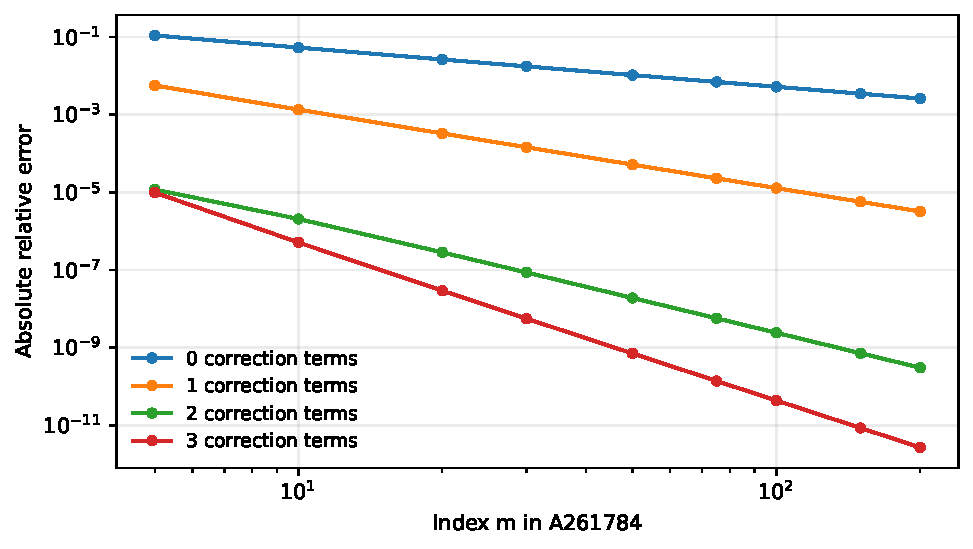
\includegraphics[width=0.87\textwidth]{figures/01-two-poisson-a261784_errors.pdf}
\caption{Absolute relative errors from the same exact data as
Table~\ref{mxc:tp:tab:errors}, with additional intermediate indices
(manuscript~01). These are numerical validations, not certified interval
error bounds.}
\label{mxc:tp:fig:errors}
\end{figure}
The very small third-order residual at $N=200$ is consistent with the
proved $O(N^{-4})$ relative remainder; between $N=100$ and $N=200$ it falls
by a factor of about $16$. It does not by itself establish that order,
which comes from the uniform analytic proof.

\section{Asymptotic inversion and integer thresholds}\label{mxc:tp:sec:inverse}

[Added 3 October 2026, batch 85B: this section is an instance of the
inversion apparatus of the repository's transseries volume \cite{tsvol}:
Proposition~\ref{mxc:tp:prop:inverse} is a first step of its perturbed
inversion, Theorem \texttt{p0:thm:perturbed-inversion}, for the core
$2x\log(\alpha x)$, and Proposition~\ref{mxc:tp:prop:threshold} is a case
of the separation condition of its staircase theorem,
\texttt{p0:thm:staircase}. Manuscript~01 does not cite either; it was
motivated by the volume's overview README, read at its pin. No novelty is
claimed for the method; the constants are specific to A261784.]

A rapidly growing sequence has a natural discrete inverse, but no unique
smooth interpolation; the two objects are kept separate.

\paragraph{A selected smooth comparator.} For fixed $J\ge1$ and
sufficiently large real $x$ define
\begin{equation}\label{mxc:tp:eq:smoothmodel}
 \mathcal A^{[J]}(x)=c_*d_*^x\frac{\Gamma(x+1)^2}{x}
 \left(1+\sum_{j=1}^{J}\beta_jx^{-j}\right).
\end{equation}
It is positive and eventually strictly increasing, because the derivative
of its logarithm is $2\log x+\log d_*+O(x^{-1})>0$. Set
\begin{equation}\label{mxc:tp:eq:inverseconst}
 \alpha=\frac{\sqrt{d_*}}e,\qquad
 \widetilde\beta_1=\beta_1+\frac16
 =-0.35514003488981599722247743640280278818\ldots.
\end{equation}
($\widetilde\beta_1$ is manuscript~01's ``$\beta_1$''; it is not Part~I's
$\beta_1$.) Stirling's expansion and~\eqref{mxc:tp:eq:diagonalall} give, at
integer $N$,
\begin{equation}\label{mxc:tp:eq:loginverse}
 \log a_N=2N\log(\alpha N)+\log(2\pi c_*)+\frac{\widetilde\beta_1}N+O(N^{-2}).
\end{equation}
The cancellation of the $\log N$ term is specific to the $(N!)^2/N$
normalization.

\begin{proposition}[Lambert-$W$ inverse and first residual correction]\label{mxc:tp:prop:inverse}
Let $Y\to\infty$ and put
\begin{equation}\label{mxc:tp:eq:inversecore}
 \Lambda=\frac{\log Y-\log(2\pi c_*)}2,\qquad
 \varpi=W_0(\alpha\Lambda),\qquad x_0=\frac\Lambda\varpi.
\end{equation}
If $x_J(Y)$ solves $\mathcal A^{[J]}(x_J)=Y$, then
\begin{equation}\label{mxc:tp:eq:inversecorrection}
 x_J(Y)=x_0-\frac{\widetilde\beta_1}{2x_0(1+\varpi)}
 +O\!\left(\frac{x_0^{-2}}{\log x_0}\right).
\end{equation}
Further terms are obtained by substituting a formal correction into the
logarithm of~\eqref{mxc:tp:eq:smoothmodel} and cancelling successive
residuals.
\end{proposition}
\begin{proof}
The definition of $\varpi$ gives $\alpha x_0=e^{\varpi}$, so
$x_0\log(\alpha x_0)=\Lambda$ and $x_0$ inverts the dominant core exactly.
Substitution in the logarithm of~\eqref{mxc:tp:eq:smoothmodel} leaves the
residual $\widetilde\beta_1/x_0+O(x_0^{-2})$. The derivative of the core
is $2(1+\log(\alpha x_0))=2(1+\varpi)$, and the displayed correction
cancels the residual to $O(x_0^{-2})$; quadratic errors in the correction
are smaller. The derivative stays comparable to $\log x_0$, and the
mean-value theorem transports the remaining logarithmic residual to the
claimed root error.
\end{proof}

\paragraph{The discrete threshold.} Define
\begin{equation}\label{mxc:tp:eq:threshold}
 \mathcal N(Y)=\min\{N\ge0:a_N\ge Y\}.
\end{equation}
The sequence $a_N$ is strictly increasing. Indeed, pad every matrix
counted by $a_N$ with a new zero row and append two columns, each having a
single~$1$ in that new row. This is an injection into the matrices counted
by $a_{N+1}$. It is not surjective: a positive one-column matrix with
$N+1$ rows and total $2N+2$ is not in its image.

\begin{proposition}[Residual brackets for integer inversion]\label{mxc:tp:prop:threshold}
For each fixed $J\ge1$ there is a constant $C_J$ such that, for all
sufficiently large $Y$, if
$\epsilon_J=C_Jx_J(Y)^{-J-1}/\log x_J(Y)$, then
\begin{equation}\label{mxc:tp:eq:thresholdbracket}
 \bigl\lceil x_J(Y)-\epsilon_J\bigr\rceil\le\mathcal N(Y)\le
 \bigl\lceil x_J(Y)+\epsilon_J\bigr\rceil.
\end{equation}
In particular $\mathcal N(Y)=\Lambda/W_0(\alpha\Lambda)+O(1)$.
\end{proposition}
\begin{proof}
At integer $N$ the logarithmic difference between $a_N$ and
$\mathcal A^{[J]}(N)$ is $O(N^{-J-1})$ by
Corollary~\ref{mxc:tp:cor:diagonal}. The derivative of
$\log\mathcal A^{[J]}$ is bounded below by a positive constant times
$\log x_J$ in a fixed-width interval around $x_J$. Choosing $C_J$ large
enough, the model's change across $\epsilon_J$ dominates that logarithmic
error at every integer in the interval. Integers strictly below
$x_J-\epsilon_J$ cannot attain $Y$; every integer at least
$x_J+\epsilon_J$ does. Monotonicity handles integers farther from the
interval. Taking ceilings gives~\eqref{mxc:tp:eq:thresholdbracket}.
\end{proof}

No unconditional formula $\mathcal N(Y)=\lceil x_J(Y)\rceil$ follows. When
the smooth root lies extremely close to an integer, even a tiny asymptotic
error can decide which of two consecutive integer thresholds is correct;
the bracket is a valid statement that does not hide that ambiguity. Its
constants are existential consequences of the asymptotic proof; no
numerically certified value of $C_J$ is claimed.

\section{Manuscript 01's checks}\label{mxc:tp:sec:checks}

Manuscript~01's program \path{code/01-two-poisson-verify.py} (delivered
as \texttt{scripts/verify.py}) uses Python integers for exact
combinatorics, SymPy for rational polynomial operations, and mpmath at 90
decimal digits for evaluation. It
(1)~matches eight displayed rows of A261781 and all fifteen displayed
terms of A261784, finite transcriptions marked as such in the source;
(2)~compares the positive Stirling transform with a separately
implemented generating-function recurrence followed by
inclusion--exclusion for every $0\le k\le n\le40$;
(3)~computes the reduced rational functions for $1\le k\le8$, checks the
denominator degrees and coprimality, and verifies later terms against the
extracted recurrence;
(4)~checks every coefficient of~\eqref{mxc:tp:eq:kernelrec} through
$n=80$, constructs $P_1$, $P_2$, $P_3$ over $\mathbb Q$, and compares the
finite Gaussian algorithm's $E_1$ with the closed
formula~\eqref{mxc:eq:dense-correction}; and
(5)~computes $a_0,\ldots,a_{200}$ exactly
(\path{data/01-two-poisson-a261784_exact.txt}) and produces the diagonal,
coverage and defect tables, which are floating-point tables, not
interval-arithmetic certificates. Its record
(\path{data/01-two-poisson-verification.json}) says ``ALL CHECKS
PASSED''. Finite tests do not prove the infinite statements; they check
algebra, indexing, normalization and implementation.

The coverage table takes $n$ to be the nearest integer to $k\log k$ and
uses the actual $h=n/k$ and $\eta=ke^{-h}$ in both approximations; the
probabilities in its third column are ratios of exact integers.
\begin{table}[htbp]
\centering\small
\begin{tabular}{@{}rrrrr@{}}
\toprule
$k$ & $n$ & Exact coverage & $e^{-\eta}$ & First correction\\
\midrule
\tableinput{data/01-two-poisson-coupon_table.tex}
\bottomrule
\end{tabular}
\caption{The first correction of~\eqref{mxc:eq:pc-zero} near the centre
of the coverage transition (manuscript~01). Rounding $n$ explains why the
leading values are not all exactly $e^{-1}$.}
\label{mxc:tp:tab:coupon}
\end{table}
The correction is not advertised as monotone in accuracy for every small
input: the theorem is a uniform asymptotic statement for bounded $s$, not
an approximation inequality for all $k$.

[Added 3 October 2026, batch 85B: at the intake's rerun on a copy,
\texttt{verify.py --max-m 200} passed all checks in 162\,s (its README
says about 16\,s), with every output byte-identical to the shipped one or
equal apart from line endings and elapsed time;
\texttt{ray\_spotchecks.py}, which imports \texttt{verify} and so needs
SymPy as well, reproduced its CSV byte for byte in 207\,s; and the figure
program reproduced the PNG pixel for pixel. The 201 computed terms of
A261784 were not compared with the OEIS b-file \cite{oeis784b}, and manuscript~01 does not
claim that they were.]

\section{Further research questions of manuscript 01}\label{mxc:tp:sec:future}

Manuscript~01 orders these by proximity to its methods, not by a claim
that any is easy or guaranteed to be new. The bracketed notes re-scope
them against Part~I.

\paragraph{Uniformity between compact rays and the coverage window.} Prove
a single relative asymptotic valid on an expanding interval such as
$1+\varepsilon\le n/k\le\log k+C$, with an error that remains informative
when coverage is exponentially rare. The kernel suggests extending
\eqref{mxc:tp:eq:kernelall} from fixed $w$ to growing $w=Lr$, while the
saddle must be controlled as $r\to\infty$; a successful result should
reproduce the polynomial corrections of
Theorem~\ref{mxc:tp:thm:couponall}, not only the limiting curve. A
concrete first step is a bound for the kernel remainder on
$|w|\le C\log n$ that keeps its exponential dependence on $|w|$.
[Added: this is the second deliverable of Research question~1 of Part~I;
open.]

\paragraph{The near-diagonal boundary.} At $n=k$ the answer is
$\mathsf F_n$, whereas the saddle variance $b$ vanishes as
$n/k\downarrow1$. Determine expansions uniform when $\ell=n-k$ is fixed,
when $\ell\to\infty$ with $\ell=o(k)$, and across their transition. The
positive Stirling sum has only $\ell+1$ summands in the fixed-$\ell$
regime, so exact polynomial descriptions may be feasible before any
saddle approximation; matching them to a large-$\ell$ saddle expansion
would complete the present analysis at the endpoint. [Added: this is the
first deliverable of Research question~1 of Part~I; open.]

\paragraph{A combinatorial realization of the latent defect.} Find a
direct decorated-matrix construction whose forgetful map induces exactly
the weights~\eqref{mxc:tp:eq:defectdef}. Ideally the defect would count a
familiar local feature and make the factor $e^{Lr/2}$ visible; such a
construction could also explain the polynomials $P_r$ and the negative
first-order term in $P_1$ without Faulhaber expansion. [Added: open; both
manuscripts decline to claim a canonical statistic.]

\paragraph{Joint laws with the number of columns.} Mark the columns by
$u$; before requiring nonzero rows the bivariate generating function is
$F_k(z;u)$ of~\eqref{mxc:eq:gf}. Study the joint distribution of the
column count and the zero-row count in the coverage window, and of the
column count together with a combinatorial defect on compact rays; the
principal pole is governed by $\log(1+1/u)$, and uniform control near
$u=1$ is needed before claiming a central limit theorem or asymptotic
independence. [Added 3 October 2026, batch 85B: the first half is
answered by Part~I. Theorem~\ref{mxc:thm:uniform} gives the uniform
control in $u$ on compact intervals, Lemma~\ref{mxc:lem:weighted-poisson}
the Poisson law under column weights, and Theorem~\ref{mxc:thm:joint} the
joint limit of the normalized column count and the zero-row count, with
independence and the conditional Gaussian law given $M=m$. On compact
rays Corollary~\ref{mxc:cor:dense-columns} gives the column central limit
theorem and its proof the exact mixture over $Q_{n,k}$; the joint law of
the column count and the defect $\Delta_{n,k}$, or a combinatorial
defect, remains open, as do the local refinements of Research
question~3.]

\paragraph{Weighted rows, columns, and restricted alphabets.} Replace the
identical row weights or the unrestricted column entries by a specified
weight system, and determine which features of the recurrence-order proof
survive when distinct factors can share poles. The proof suggests a
precise obstruction: cancellations and coincident spectra, rather than
the mere presence of a rational generating function. A classification for
finite sets of permitted column weights would be a useful structural
extension. [Added: related to Research question~8 of Part~I, which asks
the same about the coverage law; open.]

\paragraph{Beyond all algebraic orders.} The Fubini generating function
has further poles at $L+2\pi ij$. The present proofs bound their total
effect exponentially but do not extract their separate saddle
contributions. Derive those sectors, with their oscillatory phases, and
compare their scale with the late terms of the algebraic expansion; this
is where a genuinely multi-sector transseries, rather than a Poincar\'e
series, should enter, and optimal truncation and rigorous remainder
bounds would be part of that problem. [Added 3 October 2026, batch 85B:
for the Fubini numbers themselves the sectors are exact and convergent,
Theorem \texttt{q2:thm:fubini} of \cite{tsvol}; the open problem is to
carry them through the Stirling transform and the saddle. The report on
A260700 \cite{pdc} lists the same open problem for its sequence.]

\paragraph{Effective certified computation and formalization.} Make the
constants in the compact-ray error bound and
in~\eqref{mxc:tp:eq:thresholdbracket} explicit; interval estimates on the
central arc and a certified minor-arc gap could turn the inversion into a
proof-producing threshold algorithm. The exact recurrence theorem is a
suitable first formalization target: its core is pairwise disjoint simple
poles and the equivalence between rational generating functions and
eventual linear recurrences. The analytic kernel and saddle theorems are
substantially larger tasks and should be scoped separately. [Added: the
same target as Part~I's ``practical order of attack''; nothing is
formalized yet.]

\section{Hypotheses that cannot be dropped}\label{mxc:tp:sec:audit}

Manuscript~01 ends with a proof audit, kept here in full.

\paragraph{Constant versus polynomial coefficients.} The minimality
assertion is for homogeneous recurrences with constant coefficients. It is
not a lower bound for recurrences with polynomial coefficients in $n$,
nonlinear recurrences, or recurrences involving several columns $k$ at
once.

\paragraph{Nonnegative versus strictly positive entries.} Entries are
nonnegative; the restrictions are on entire rows and columns, not on each
cell. Replacing cells by positive integers changes the generating
functions and the sequence.

\paragraph{The polynomial part of a rational function.} The
fixed-spectrum formula for $A(n,k)$ applies to $n\ge1$, and the
recurrence for $T(n,k)$ starts after the numerator has ceased
contributing. Ignoring either point creates incorrect initial conditions.

\paragraph{Positivity before relative error transport.} The approximation
of $\mathsf F_q$ is transported through the positive
identity~\eqref{mxc:eq:stirling}, not through the alternating
inclusion--exclusion sum: an exponentially accurate approximation term by
term in an alternating sum need not be relatively accurate after
cancellation. The coverage calculation instead controls factorial moments
and then uses Bonferroni truncation.

\paragraph{Compactness in the ray theorem.} The uniform constants require
$n/k$ to stay away from $1$ and infinity. Neither endpoint is covered by
substituting it in~\eqref{mxc:tp:eq:Bnk}, and the actual rational $n/k$
must be used when $n$ is rounded.

\paragraph{Two different Poisson variables.} $M$ counts zero rows in
uniformly sampled matrices that may have zero rows; $\Delta_{n,k}$ is an
auxiliary variable defined by positive transform weights. Their means,
parameter regimes and sample spaces are different.

\paragraph{Formal Gaussian algebra.} The
prescription~\eqref{mxc:eq:saddle-algorithm} means coefficient extraction
first, Gaussian evaluation second; it does not require the integral of
the untruncated exponential expression to converge.

\paragraph{Asymptotic expansion versus convergent series.} Every order $J$
is fixed before the size parameter tends to infinity. Neither growth
estimates for the coefficients as $J\to\infty$ nor optimal truncation are
asserted.

\paragraph{Numerics and proof status.} Exact integer checks certify their
finite inputs. The 90-digit numerical calculations are independent
consistency checks, not rigorous floating-point enclosures or a
machine-checked proof of the theorems.

\section{Manuscript 01's draft OEIS additions (not submitted)}\label{mxc:tp:sec:oeis}

Manuscript~01 includes draft additions to two OEIS entries, shipped as
\path{data/01-two-poisson-OEIS_updates_draft.txt}. \emph{They were not
submitted}, by manuscript~01 or by this report; manuscript~01 itself asks
for independent review and a stable public manuscript link first, and for
the earlier source and conjecture attributions to be preserved. Their
substance, in this report's letters:

\paragraph{A261781.} For $k>0$ the reduced denominator of the ordinary
generating function of column $k$ is $\prod_{j=1}^k(2(1-x)^j-1)$, so its
minimal eventual homogeneous constant-coefficient recurrence has order
$k(k+1)/2$: inclusion--exclusion expresses the column generating function
as the alternating binomial sum of $(1-x)^j/(2(1-x)^j-1)$, whose $j$th
summand has simple poles at $1-2^{-1/j}e^{2\pi i\ell/j}$, and different
summands have disjoint pole sets. The fixed-column constants are
$c_k=1/(2k(2^{1/k}-1))$ and $d_k=1/(1-2^{-1/k})$, and $d_{k+1}-d_k$
increases strictly to $1/\log2$, with $d'(x)$ as
in~\eqref{mxc:tp:eq:dprime}. Attribution should retain the existing
conjecture attribution and cite the generating-function source.

[Added 3 October 2026, batch 85B: \emph{before any use} this draft must be
corrected as in Section~\ref{mxc:tp:sec:novelty}. Its sentence saying
that these statements prove the two claims labelled conjectures overstates
them: a recurrence of order $k(k+1)/2$ with this denominator is
\cite[Proposition~25]{mpr2009}, with the case $k=2$ in Remark~26, and the
limit follows from Proposition~13 there; what is new is the minimality
and the strict monotonicity. The shipped file is kept byte-identical and
still contains the overstated sentence.]

\paragraph{A261784.} With $L=\log2$ and $r=2+W_0(-2e^{-2})$, the posted
prefactor is $c_*=2^{r/2}/(4\pi L\sqrt{r-1})$ and the growth rate
$d_*=4/(L^2r(2-r))$; the relative correction begins
$1+\beta_1/N+\beta_2/N^2+\beta_3/N^3$ with the values of
Section~\ref{mxc:tp:sec:diagonal} (the draft's index $n$ is $N$ here). The
decimals evaluate finite exact prescriptions and are not fitted. The
leading asymptotic already in the entry, Kot\v{e}\v{s}ovec's
(18~February 2017, updated 20~April 2024), is not to be presented as new,
nor described as labelled a conjecture.

\addcontentsline{toc}{part}{Appendix}
\appendix
\section{Provenance and editorial notes}\label{mxc:app:provenance}

[Added 3 October 2026, batch 85B.]

\paragraph{Sources.} The report was built from two manuscripts of batch~85
of ProveIt's incoming-reports intake, written independently on the same
subject.
\begin{itemize}
\item \emph{Manuscript~06} (Part~I, the base): the archive
 \nolinkurl{Matrix_Compositions_Uniform_Asymptotics.zip} (21~files), main
 file \texttt{matrix\_compositions.tex} (2,078 lines, 100 labels), a
 31-page PDF titled \emph{Matrix Compositions: Exact Spectra, Hankel
 Products, and Uniform Asymptotics}, dated October~3, 2026 (Pacific time).
 Its author line and PDF metadata read ``OpenAI ChatGPT'', with ``Research
 prepared for Vladimir Reshetnikov''. Its pin is the search-index commit
 \texttt{ce37e13f4aa16819c87c3ccc611362d15758f2ac} (2026-10-03, 17:05)
 \cite{proveit}. It arrived in commit \texttt{345284ac8}.
\item \emph{Manuscript~01} (Part~II): the archive
 \nolinkurl{OEIS_Matrix_Compositions_Research.zip} (26~files), main file
 \texttt{matrix\_compositions.tex} (1,561 lines, 98 labels), a 22-page PDF
 titled \emph{Matrix compositions: finite spectra, uniform asymptotics,
 and two Poisson limits}, dated 3~October 2026, author line ``Research
 report prepared for Vladimir Reshetnikov''. Its pin is the tree revision
 \texttt{d68b65ea064084fb121df9bb431b21d086f7be81}; it also records the
 search-index commit \texttt{ce37e13f4} \cite{proveit01}. It arrived in
 commit \texttt{317c1ce2e}, with the other archives of batch~85; the
 placement of batch~85A (\texttt{713149ded}) held it back so that it could
 be merged with manuscript~06.
\end{itemize}
Both were placed together by commit \texttt{fa2f3e419}, which deleted both
archives from \texttt{docs/incoming}; they survive in their arrival
commits. Neither manuscript is an edition of the other: they share about
0.7\,\% and 0.5\,\% of their word 8-grams (bibliography entries and one
phrase), and their pins, code and notation differ.

\paragraph{Why manuscript~06 is the base.} On every theorem the two share,
manuscript~06 has the weaker hypotheses or the more general statement:
recurrence minimality for every column weight $u>0$ (manuscript~01:
$u=1$); a pole bound uniform in $k$, also weighted (manuscript~01: a
factor $k-1$); the coverage expansion of the whole generating function
in complex $w$ (manuscript~01: $\Pp(M=0)$ only); and the correct
attribution of the recurrence's existence to \cite[Proposition~25]{mpr2009}.
It also has more new mathematics (the Hankel determinant product, the
sharp total-variation rate, the joint Gaussian--Poisson law, the column
central limit theorem, the prescribed-column threshold). Manuscript~01 is
more general only in the kernel lemma, and that lemma only serves compact
rays, where both theorems coincide.

\paragraph{Where the merge had to choose.}
\begin{itemize}
\item Shared results are printed once, in manuscript~06's form, with a
 bracketed note naming manuscript~01's version
 (Table~\ref{mxc:tp:tab:routes}). Manuscript~01's proofs that are the same
 argument are summarized in those notes, not reprinted; its genuinely
 different devices are recorded there (Bonferroni truncation for the
 coverage probability, the tail bound $|\mathsf W_n(w)|\le e^{|w|}$, the
 direct uniqueness argument for the maximum on the circle) or printed in
 Part~II where a new result needs them.
\item Manuscript~01's $k$-dependent pole bound is printed as
 Remark~\ref{mxc:rem:uniform-ms01}, because it is sharper for $k\le4$.
\item Manuscript~01's kernel theorem is printed in full in Part~II as the
 general form of Lemma~\ref{mxc:lem:kernel}, and
 Remark~\ref{mxc:rem:kernel-untruncated} says so where the lemma stands.
 Manuscript~06's lemma is kept unchanged.
\item Manuscript~06's moments of $D$ in Corollary~\ref{mxc:cor:dense-columns}
 are kept, with a pointer to the stronger Theorem~\ref{mxc:tp:thm:defect}.
\item Manuscript~01's closed form of $\beta_1$ is printed as a note after
 Corollary~\ref{mxc:cor:784}, being the same expression; its fifty-digit
 constants and $\beta_3$ are in Part~II.
\item Manuscript~01's overstated claim about the order conjecture is
 narrowed (Section~\ref{mxc:tp:sec:novelty}), its draft OEIS text is
 printed with the correction (Section~\ref{mxc:tp:sec:oeis}), and its
 example~\eqref{mxc:eq:smallexamples} is credited to
 \cite[Remark~26]{mpr2009}.
\item Manuscript~01's research question on joint column laws is
 re-scoped as partly answered by manuscript~06; manuscript~06's Research
 question~2 is re-scoped as answered for the event $M=0$ by
 Theorem~\ref{mxc:tp:thm:couponall}.
\item Manuscript~01's inversion section is printed with a note that it is
 an instance of the transseries volume's apparatus; manuscript~01's source
 manifest (its Appendix~C) is replaced by this appendix and the report
 README, and its rebuild instructions by the README.
\item Manuscript~01's three tables (Tables~\ref{mxc:tp:tab:defect},
 \ref{mxc:tp:tab:errors} and~\ref{mxc:tp:tab:coupon}) are typeset,
 unchanged, from its shipped table bodies, the files
 \texttt{data/01-two-poisson-X.tex} with \texttt{X} one of
 \texttt{defect\_table}, \texttt{error\_table} and
 \texttt{coupon\_table}. Its fourth body, \texttt{diagonal\_table}
 (the same diagonal errors at more indices and digits), was not used by
 its article and is not used here.
\end{itemize}

\paragraph{What the write changed in manuscript~06's text.}
\begin{itemize}
\item Every label gained the prefix \texttt{mxc:} (100 labels; every
 reference was updated); nothing was renamed otherwise and nothing was
 removed.
\item Added: the second author and date lines of the title, the PDF
 metadata, the editorial note after the abstract, the part heading,
 Section~\ref{mxc:sec:dictionary} with Table~\ref{mxc:tab:dictionary},
 Remarks~\ref{mxc:rem:minimal-sources}, \ref{mxc:rem:uniform-ms01}
 and~\ref{mxc:rem:kernel-untruncated}, bracketed notes marked
 ``[Added 3 October 2026, batch 85B]'' in Sections~\ref{mxc:sec:scope},
 \ref{mxc:sec:exact}, \ref{mxc:sec:poisson}, \ref{mxc:sec:dense},
 \ref{mxc:sec:numerics} and~\ref{mxc:sec:questions}, Part~II, this
 appendix, and five bibliography entries
 \cite{proveit01,pdc,tsvol,leanob,oeis784b}.
\item The figure path is now \path{figures/06-hankel-coupon_window.pdf}.
\item No delivered sentence of manuscript~06 was changed or removed. Every
 non-claim is kept: the abstract's last sentence; the scope table's
 caption; the bounded audit; ``The theorem controls the unrestricted count
 $A(n,k)$ uniformly'' and what it does not say; the moving-mean remark;
 the compactness paragraph after Corollary~\ref{mxc:cor:dense-columns};
 the prescribed-column caveat; the Hankel caveat on total positivity; the
 numerics caveats; and the caveat on the research questions.
\end{itemize}
Manuscript~01's text is restated in manuscript~06's letters
(Table~\ref{mxc:tab:dictionary}), with some proofs condensed; none of its
statements was strengthened, and every one of its non-claims is kept
(Section~\ref{mxc:tp:sec:front}, the remarks after
Theorems~\ref{mxc:tp:thm:couponall} and~\ref{mxc:tp:thm:defect},
Remark~\ref{mxc:tp:rem:floors}, Sections~\ref{mxc:tp:sec:inverse},
\ref{mxc:tp:sec:checks}, \ref{mxc:tp:sec:audit} and~\ref{mxc:tp:sec:oeis}).

\paragraph{Overloaded letters in manuscript~06.} Manuscript~06 reuses some
letters; none is renamed, and in each case the section determines the
meaning. $D$ is $\binom{k+1}2$ in Section~\ref{mxc:sec:exact}, the constant
$D_u=16b/L_u^2$ in Section~\ref{mxc:sec:uniform}, the function $D(\eta)$ in
Section~\ref{mxc:sec:poisson} and $n-Q$ in
Section~\ref{mxc:sec:dense-columns}. $d$ is $\binom{k+1}2$ and $c$ is
$\binom{k+1}3$ in Section~\ref{mxc:sec:hankel}, beside the growth
constants $d_k$, $c_k$. $b$ is $u/(1+u)$ in
Sections~\ref{mxc:sec:exact}--\ref{mxc:sec:uniform}, also $u$ in
Section~\ref{mxc:sec:hankel}, the variance $\kappa_2$ in
Section~\ref{mxc:sec:dense}, and $b_j$ are factorial moments.
$P_j(t)$ in Section~\ref{mxc:sec:hankel} and $P_j(w)$ in
Section~\ref{mxc:sec:allorders} are different polynomials; $E_n(w)$ is a
product, $E_j(\lambda)$ a saddle coefficient and $E_n=B\rho^{n-1}$ an error
budget; $r$ is $r_k=1-a_k$, the saddle, and a summation index; $v$ is $Lr/2$
in Section~\ref{mxc:sec:dense} but a tilting parameter in the proof of
Theorem~\ref{mxc:thm:joint}; and $m$ indexes $d_m$ and counts columns.

\paragraph{Checks by the intake.} The placement reran both packages on
copies: manuscript~06's suite passed with its outputs byte-identical or
equal apart from line endings and timings and its figure pixel-identical;
manuscript~01's suite passed likewise, and its checksum ledger matched
25/25. Manuscript~06's diagonal constants and manuscript~01's agree in
every printed digit, and their coverage probabilities at $k=20$, $n=60$
agree. The intake also verified Proposition~25 and Remark~26 in the
published paper, the impulse of Remark~\ref{mxc:rem:impulse} at $k=1,2$,
the instances $H_{3,s}(u)$, $H_{2,1}(1)=8$ and $H_{3,1}(1)=62208$, the
constants of Theorem~\ref{mxc:thm:uniform} and
Remark~\ref{mxc:rem:uniform-ms01}, the moments in
Corollary~\ref{mxc:cor:dense-columns}, the increment
expansion~\eqref{mxc:eq:d-incr}, the cumulant recursion at $j=3$, and
$P_3$ numerically. These checks do not replace an independent review of
the proofs.

\begin{thebibliography}{99}
\raggedright
\bibitem{oeis780} The OEIS Foundation Inc., \emph{The On-Line Encyclopedia of
Integer Sequences}, entry A261780, created by Alois P. Heinz.
\url{https://oeis.org/A261780}. Accessed October 3--4, 2026.
\bibitem{oeis781} The OEIS Foundation Inc., entry A261781, created by
Alois P. Heinz; conjecture comments by V\'aclav Kot\v{e}\v{s}ovec,
October 14, 2017. \url{https://oeis.org/A261781}.
Accessed October 3--4, 2026.
\bibitem{oeis784} The OEIS Foundation Inc., entry A261784, created by
Alois P. Heinz; asymptotic formula by V\'aclav Kot\v{e}\v{s}ovec,
February 18, 2017, updated April 20, 2024.
\url{https://oeis.org/A261784}. Accessed October 3--4, 2026.
\bibitem{mpr2009} E. Munarini, M. Poneti, and S. Rinaldi,
\emph{Matrix Compositions}, Journal of Integer Sequences \textbf{12}
(2009), Article 09.4.8, 28 pp.
\url{https://cs.uwaterloo.ca/journals/JIS/VOL12/Rinaldi/rinaldi.pdf}.
\bibitem{mpr2006} E. Munarini, M. Poneti, and S. Rinaldi,
\emph{Matrix compositions}, Proceedings of FPSAC 2006, San Diego,
pp.~445--456. \url{https://garsia.math.yorku.ca/fpsac06/papers/49.pdf}.
\bibitem{louchard} G. Louchard, \emph{Matrix compositions: a probabilistic
analysis}, Pure Mathematics and Applications \textbf{19} (2008),
nos.~2--3, 127--146. Author's long version dated July 10, 2008:
\url{https://guy.louchard.web.ulb.be/louchard.papers/compmat.ps}.
Publication list: \url{https://guy.louchard.web.ulb.be/index_old.htm}.
\bibitem{proveit} V. Reshetnikov, \emph{ProveIt}, public research and
formalization repository. \url{https://github.com/VladimirReshetnikov/ProveIt}.
Indexed snapshot observed in this audit:
\texttt{ce37e13f4aa16819c87c3ccc611362d15758f2ac}.
\bibitem{oeis784b} The OEIS Foundation Inc., b-file of A261784.
\url{https://oeis.org/A261784/b261784.txt}. Identified by manuscript~01;
not compared in full by either manuscript.
\bibitem{proveit01} V. Reshetnikov, \emph{ProveIt}, series-and-transseries
overview, \path{Analysis/Transseries/docs/series-and-transseries/README.md},
read by manuscript~01 at revision
\texttt{d68b65ea064084fb121df9bb431b21d086f7be81} (blob
\texttt{7bdc83aeb}); its indexed searches exposed
\texttt{ce37e13f4aa16819c87c3ccc611362d15758f2ac}.
\url{https://github.com/VladimirReshetnikov/ProveIt}.
\bibitem{pdc} ProveIt research-report collection, \emph{All fixed order
asymptotics for distinct parabolic double cosets} (OEIS A260700),
\path{SetTheory/Cardinals/docs/reports/generating-functions-and-asymptotics/oeis-sequence-asymptotics/a260700-parabolic-double-cosets/},
label prefix \texttt{pdc:}.
\bibitem{tsvol} ProveIt, \emph{Transseries and inversion} (the canonical
series-and-transseries volume),
\path{Analysis/Transseries/docs/series-and-transseries/Transseries_And_Inversion/transseries_and_inversion.tex};
Theorems \texttt{q2:thm:fubini} (exact pole-lattice transseries of the
Fubini numbers), \texttt{p0:thm:perturbed-inversion} and
\texttt{p0:thm:staircase}.
\bibitem{leanob} ProveIt, Lean module
\path{Analysis/FabiusFunction/Lean/FabiusFunction/OrderedBell.lean}:
\texttt{Fabius.fubini}, \texttt{Fabius.egfA\_fubini},
\texttt{Fabius.two\_sub\_exp\_mul\_egfA\_fubini}.
\end{thebibliography}
\end{document}
